\documentclass[12pt]{ctexart}   %using XeLatex for build it.
\usepackage[utf8]{inputenc}


\CTEXsetup[format={\Large\bfseries}]{section} %设置Section左对齐。

\title{ Computer Network }
\author{Santiago}
\date{May 1, 2020}

\usepackage{natbib} % for reference.
\usepackage{graphicx} % for images.
\usepackage{subfigure} % for subfigure.
\usepackage{float} 
\usepackage{xcolor}  %彩色字,color包亦可。
\usepackage{framed} %文字背景颜色
\usepackage[colorlinks,linkcolor=blue]{hyperref} %超链接,蓝色。
\usepackage{courier} % for code style word.

\usepackage{colortbl,booktabs}%定义了几个*rule,表格

\usepackage{adjustbox} %子页对齐

\usepackage{amsmath} %数学公式格式
\usepackage{amssymb} % 数学公式格式

\pagestyle{plain}  % 添加页码

\usepackage{listings}
\lstset { %
    language=C++,
    backgroundcolor=\color{black!5}, % set backgroundcolor
    basicstyle=\footnotesize,% basic font setting
}


\begin{document}
\maketitle %渲染Title。

\begin{abstract}
	Prof.David Wetherall from University of Washington \\
	Computer Network Course 
\end{abstract}

\section{Week 1 - Goals and Motivation}
	\subsection{网址}
	\begin{itemize}
		\item Total Course: 
		\begin{itemize}
			\item https://media.pearsoncmg.com/ph/streaming/esm/tanenbaum5e\_videonotes/ \\
			tanenbaum\_videoNotes.html
		\end{itemize}
		\item Week1~Weel5 
		\begin{itemize}
			\item https://www.youtube.com/playlist?list=PLzmjQ4eaGEug9YlLvqpBTdVyIZhzQxTzu
		\end{itemize}
		\item Week6~Week10
		\begin{itemize}
			\item	https://www.youtube.com/playlist?list=PLv4Qy0s26-PL2-tAs6mPaxUzq-wwMdv5Y
		\end{itemize}
	
	\end{itemize}
	\subsection{The Main Point}
	\begin{itemize}
		\item To learn how the Internet works
		\begin{itemize}
			\item What really happens when you "browse the web"?
			\item What are TCP/IP, DNS, HTTP, NAT, VPNs, 802.11 etc. anyway?
		\end{itemize}		 
		\item To learn the fundamentals of computer network.
		\begin{itemize}
			\item What hard problems must they solve?
			\item What design strategies have proven valuable?
		\end{itemize}
	\end{itemize}

\section{Week 1 - Uses of Networks}
	\subsection{Statistical Multiplexing}
	
	\begin{figure}[h!] % h for here.
	 \centering
	 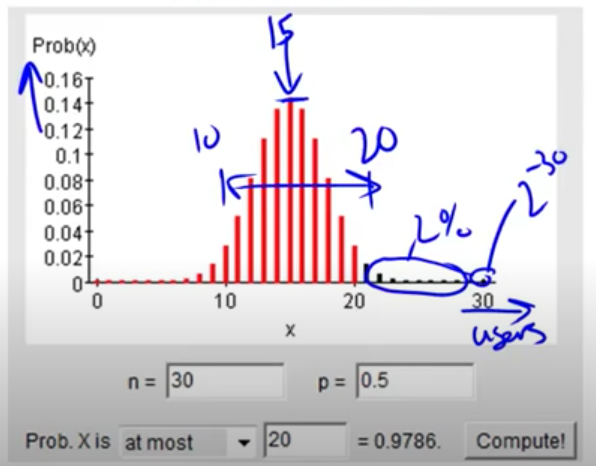
\includegraphics[scale=1.0]{images/1-2-1}
	\caption{ Binomial Calculator }
	 \label{fig:1-2-1}
	 \end{figure}
	
	\begin{itemize}
		\item Sharing of network bandwidth between users according to the statistic of their demand
		\begin{itemize}
			\item (\underline{Multiplexing} just means sharing)
			\item Useful because users are mostly idle and their traffic is bursty
		\end{itemize}
		
		\item Key question:
		\begin{itemize}
			\item How much does it help?
		\end{itemize}
		
		\item See Figure~\ref{fig:1-2-1}
		
		\item With 30 independent users, still unlikely (20\& chance) to need more than 100 Mbps!
		\begin{itemize}
			\item Binomial probabilities
		\end{itemize}
		
		\item Can serve more users with the same size network
		\begin{itemize}
			\item Statistical multiplexing gain is 30/20 or 1.5X
			\item But may get unlucky; users will have degraded service
		\end{itemize}
		
	\end{itemize}
	
	\subsection{For Content Delivery}
	
	
		%\begin{% figure 1 & 2
		\begin{figure}
			\begin{minipage}[t]{0.5\linewidth}
				\centering
				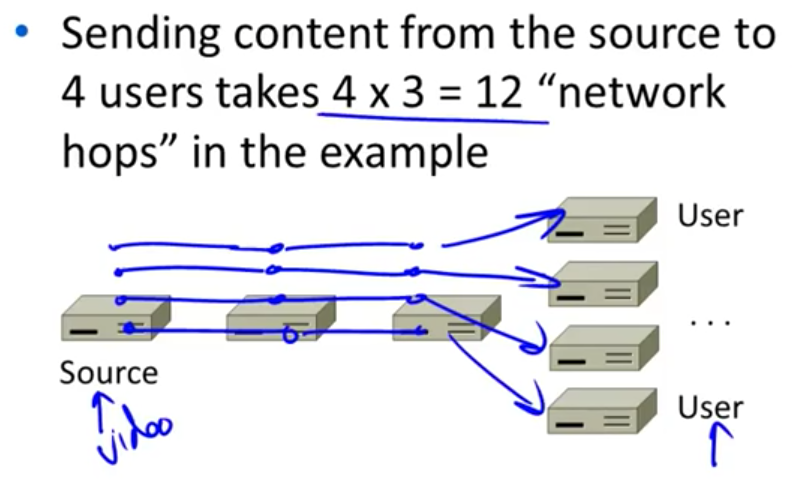
\includegraphics[width=2.2in]{images/1-2-2}
				\caption{Sending content from the source to 4 users}
				\label{fig:1-2-2}
			\end{minipage}
			\begin{minipage}[t]{0.5\linewidth}
				\centering
				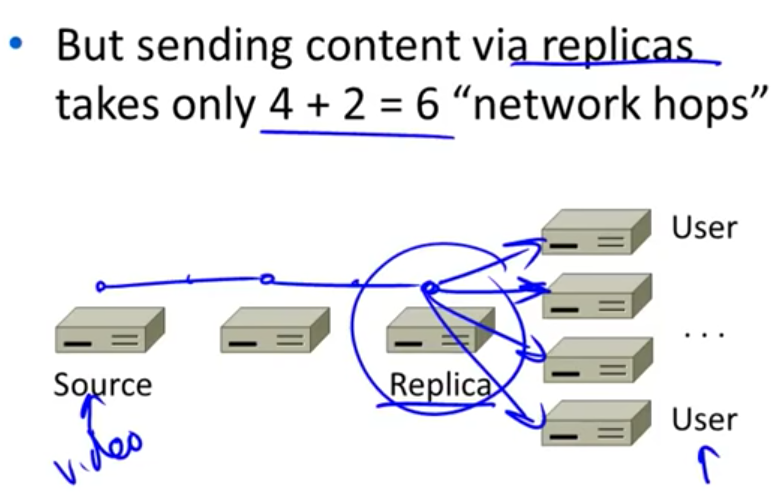
\includegraphics[width=2.2in]{images/1-2-3}
				\caption{sending content via replicas}
				\label{fig:1-2-3}
			\end{minipage}
		\end{figure}
	
	
	\begin{itemize}
		\item Same content is delivered to many users
		\begin{itemize}
			\item Videos (large), songs, apps and upgrades, web pages, ...
		\end{itemize}
		
		\item More efficient then sending a copy all the way to each user
		\begin{itemize}
			\item Uses replicas to the network
		\end{itemize}
		
		\item Sending content from the source to 4 users takes \underline{$4 \times 3=12$} "network hops" in the example, See Figure~\ref{fig:1-2-2}
		\item But sending content via replicas takes only \underline{$4+2=6$} "network hops", See Figure~\ref{fig:1-2-3}
	\end{itemize}
	
	\subsection{The Value of Connectivity}
	
	\begin{figure}[h!] % h for here.
	 \centering
	 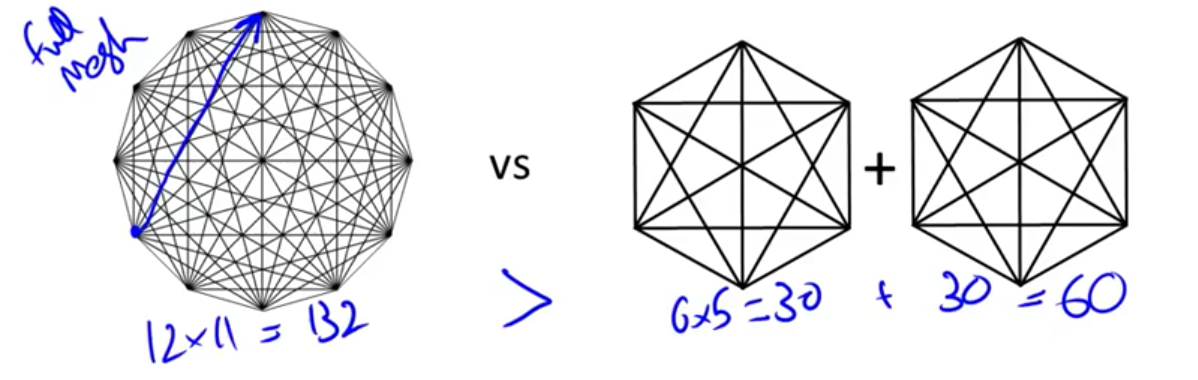
\includegraphics[scale=0.5]{images/1-2-4}
	\caption{ The Value of Connectivity }
	 \label{fig:1-2-4}
	 \end{figure}	
	
	\begin{itemize}
		\item "Metcalfe's Law" ~1980:
		\begin{itemize}
			\item The value of a network of N nodes is proportional to $N^2$
			\item Large networks are relatively more valuable than small ones
		\end{itemize}
		
		\item Example: both side have \underline{12 nodes}, but the left network has more connectivity, See Figure~\ref{fig:1-2-4}
	\end{itemize}
	
\section{Week 1 - Network Components}
	\subsection{Component Names}
	
	\begin{figure}[h!] % h for here.
	 \centering
	 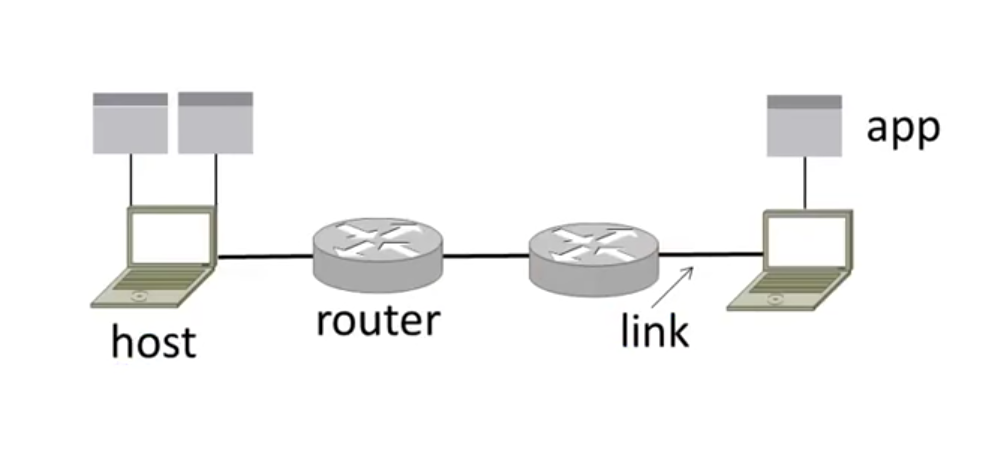
\includegraphics[scale=1.0]{images/1-3-1}
	\caption{ Parts of a Network }
	 \label{fig:1-3-1}
	 \end{figure}
	 
	\begin{itemize}
		\item See Figure~\ref{fig:1-3-1}
		\item Component Names, See Table~\ref{table:1-3-1}
		%%% 开始表格
		\begin{table}[h] %开始一个表格environment,表格的位置是h,here。
		\begin{center}
		\begin{tabular}{p{5cm}|p{3cm}|p{3cm}} %设置了每一列的宽度,强制转换。
		\hline
		\hline
		Component & Function & Example \\ %用&来分隔单元格的内容 \\表示进入下一行
		\hline %画一个横线,下面的就都是一样了,这里一共有4行内容
		\underline{ Application}, or app, user & Uses the network & Skype, iTunes, Amazon\\
		\hline
		 \underline{Host}, or end-system, edge device, node, source, sink & Supports apps & Laptop, mobile, desktop\\
		\hline
		\underline{Router}, or switch, node, hub, intermediate system & Relays messages between links & Access point, cable/DSL modem\\
		\hline
		\underline{Link}, or channel & Connects nodes & Wires, wireless\\
		\hline
		\hline
		\end{tabular}
		\end{center}
		\caption{Component Names} %显示表格的标题
		\label{table:1-3-1}
		\end{table}
		%%% 结束表格
	\end{itemize}
	
	\subsection{Types of Links}
	
	%\begin{% figure 1 & 2
		\begin{figure}
			\begin{minipage}[t]{0.3\linewidth}
				\centering
				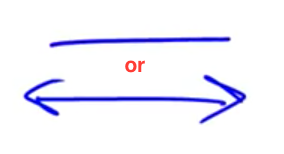
\includegraphics[width=1.5in]{images/1-3-2}
				\caption{Full-duplex}
				\label{fig:1-3-2}
			\end{minipage}
			\begin{minipage}[t]{0.3\linewidth}
				\centering
				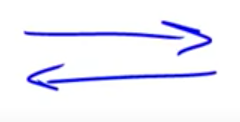
\includegraphics[width=1.5in]{images/1-3-3}
				\caption{Half-duplex}
				\label{fig:1-3-3}
			\end{minipage}
			\begin{minipage}[t]{0.3\linewidth}
				\centering
				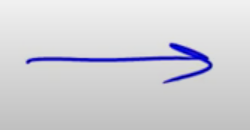
\includegraphics[width=1.5in]{images/1-3-4}
				\caption{Simplex}
				\label{fig:1-3-4}
			\end{minipage}
		\end{figure}
		
	\begin{itemize}
		\item \underline{Full-duplex}
		\begin{itemize}
			\item Bidirectional, See Figure~\ref{fig:1-3-2}
		\end{itemize}
		
		\item \underline{Half-duplex}
		\begin{itemize}
			\item Bidirectional, Figure~\ref{fig:1-3-3}
		\end{itemize}
		
		\item \underline{Simplex}
		\begin{itemize}
			\item unidirectional, See Figure~\ref{fig:1-3-4}
		\end{itemize}
		
	\end{itemize}
	
	\subsection{Wireless Links}
	
	%\begin{% figure 1 & 2
		\begin{figure}
			\begin{minipage}[t]{0.5\linewidth}
				\centering
				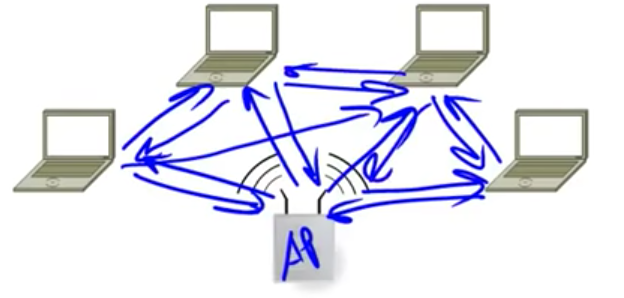
\includegraphics[width=2.2in]{images/1-3-5}
				\caption{Message is \underline{broadcast}}
				\label{fig:1-3-5}
			\end{minipage}
			\begin{minipage}[t]{0.5\linewidth}
				\centering
				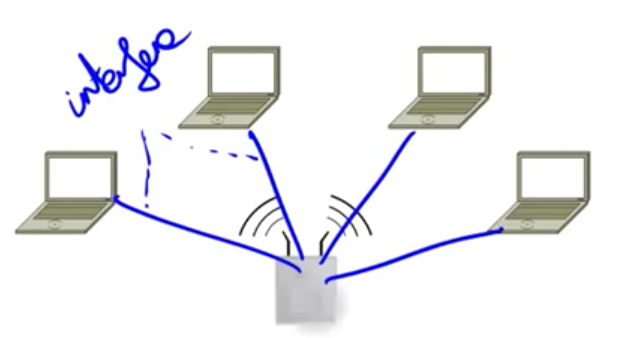
\includegraphics[width=2.2in]{images/1-3-6}
				\caption{show logical links}
				\label{fig:1-3-6}
			\end{minipage}
		\end{figure}
		
	\begin{itemize}
	\item Message is \underline{broadcast}, See Figure~\ref{fig:1-3-5}
	\begin{itemize}
		\item Received by all nodes in range
		\item Not a good fit with our model
	\end{itemize}
	
	\item Often show logical links, See Figure~\ref{fig:1-3-6}
	\begin{itemize}
		\item Not all possible connectivity
	\end{itemize}
	\end{itemize}

\section{Week 1 - Sockets}
	\subsection{Network-Application Interface}
	
	\begin{figure}[h!] % h for here.
	 \centering
	 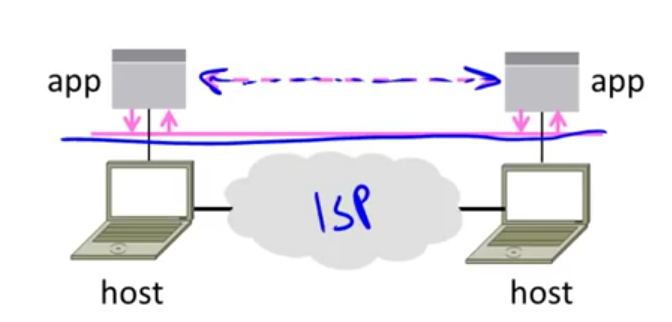
\includegraphics[scale=1.0]{images/1-4-1}
	\caption{ Network-Application Interface }
	 \label{fig:1-4-1}
	 \end{figure}
	 
	\begin{itemize}
		\item Defines how apps use the Network, See Figure~\ref{fig:1-4-1}
		\begin{itemize}
			\item Lets apps talk to each other via hosts; hides the detail of the net work
		\end{itemize}
	\end{itemize}
	
	\subsection{Socket API}
	
	\begin{figure}[h!] % h for here.
	 \centering
	 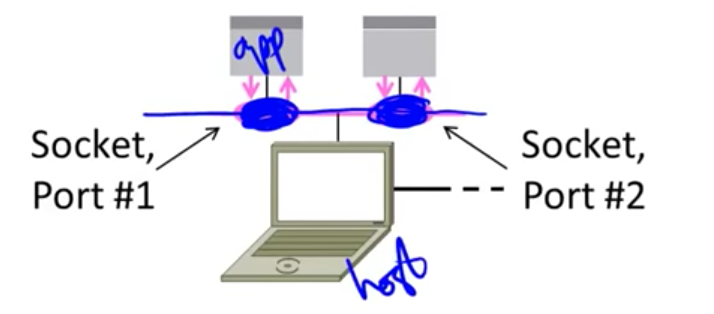
\includegraphics[scale=1.0]{images/1-4-2}
	\caption{ Socket API }
	 \label{fig:1-4-2}
	 \end{figure}
	 
	 \begin{figure}[h!] % h for here.
	 \centering
	 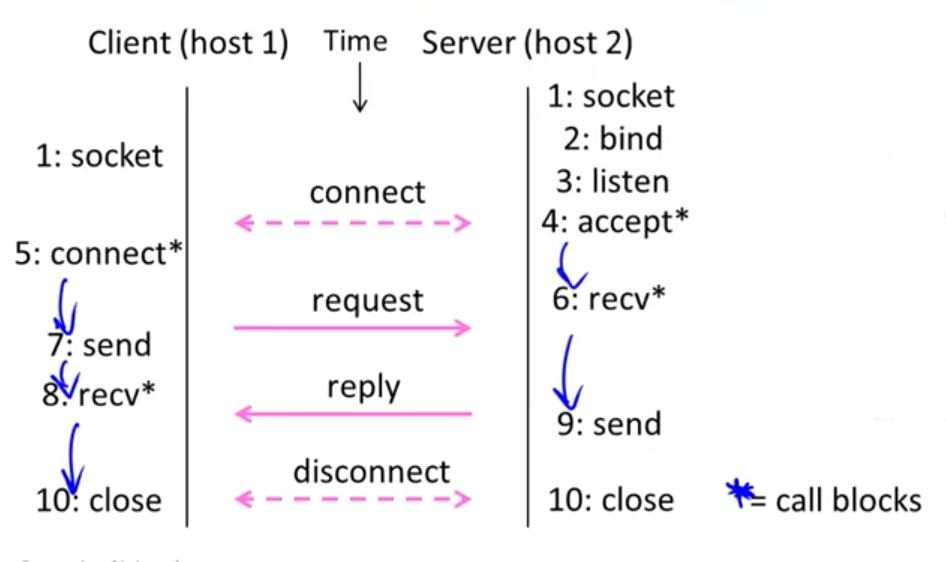
\includegraphics[scale=1.0]{images/1-4-3}
	\caption{ Using Sockets }
	 \label{fig:1-4-3}
	 \end{figure}
	 
	\begin{itemize}
		\item Simple abstraction to use the network
		\begin{itemize}
			\item The network service API used to write all Internet applications
			\item Part of all major OSes and languages; originally Berkeley (Unix) ~1983
		\end{itemize}
		
		\item Supports two kinds of network services
		\begin{itemize}
			\item Streams: reliably send a stream of bytes
			\item Datagrams: unreliably send separate messages. (Ignore for now.)
		\end{itemize}
		
		\item \underline{Sockets} let apps attach to the local network at different \underline{ports} , See Figure~\ref{fig:1-4-2}
		
		\item Socket API Functions, See Table~\ref{table:1-4-1}
		%%% 开始表格
		\begin{table}[h] 
		\begin{center}
		\begin{tabular}{p{3cm}|p{9cm}} 
		\hline
		\hline
		Primitive & Meaning \\
		\hline 
		SOCKET & Create a new communication endpoint\\
		\hline
		 BIND & Associate a local address with a socket\\
		\hline
		LISTEN & Announce willingness to accept connections; give queue size\\
		\hline
		ACCEPT & Passively establish an incoming connection\\
		\hline
		CONNECT & Actively attempt to establish a connection \\
		\hline
		SEND & Send some data over the connection \\
		\hline
		RECEIVE & Receive some data from the connection \\
		\hline
		CLOSE & Release the connection \\
		\hline
		\hline
		\end{tabular}
		\end{center}
		\caption{Socket API Functions} 
		\label{table:1-4-1}
		\end{table}
		%%% 结束表格
		
		\item Using Sockets, See Figure~\ref{fig:1-4-3}
	\end{itemize}
	
\section{Week 1 - Traceroute}
	\subsection{Traceroute}
	
	\begin{figure}[h!] % h for here.
	 \centering
	 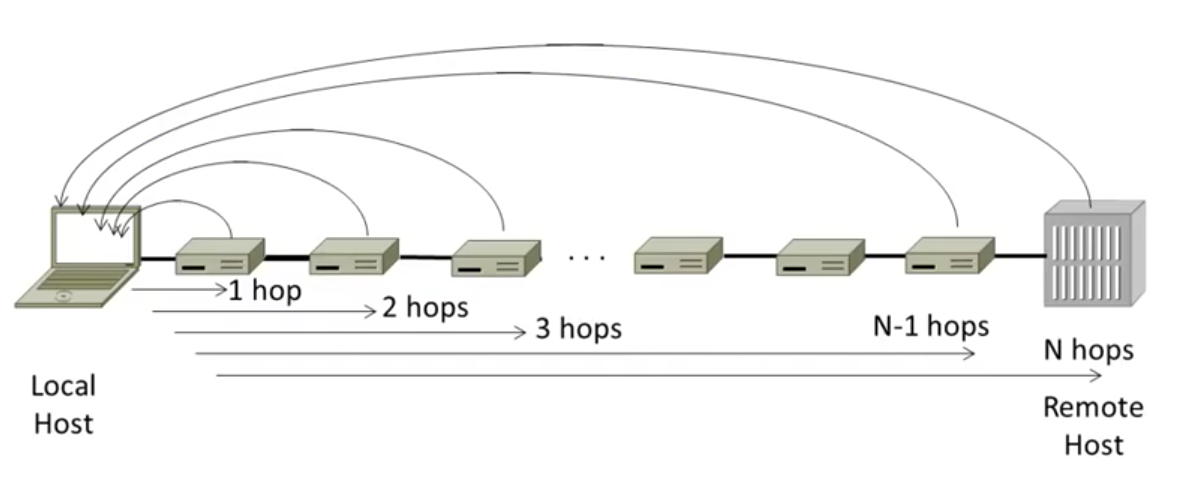
\includegraphics[scale=0.7]{images/1-5-1}
	\caption{ Traceroute }
	 \label{fig:1-5-1}
	 \end{figure}
	 
	 \begin{figure}[h!] % h for here.
	 \centering
	 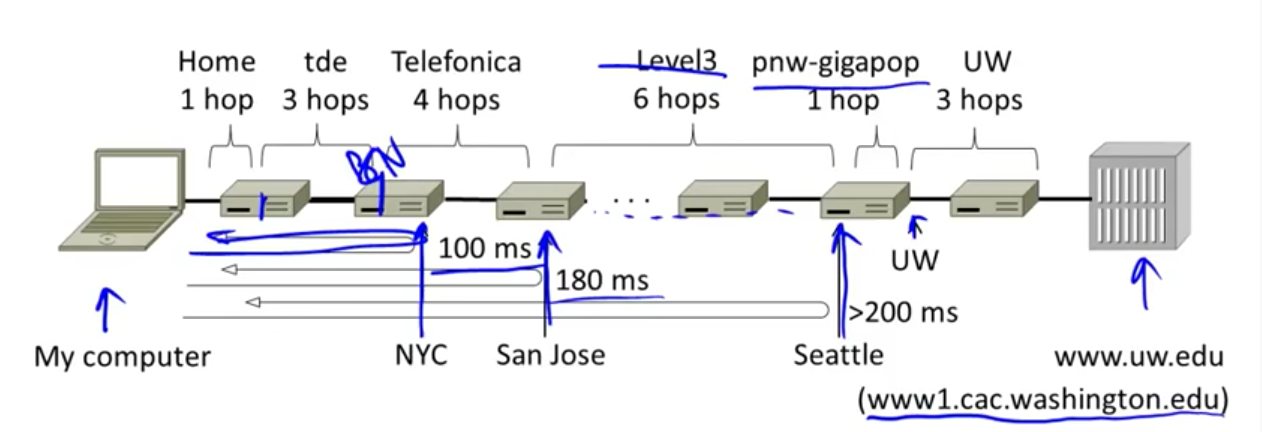
\includegraphics[scale=0.7]{images/1-5-2}
	\caption{ Using Traceroute }
	 \label{fig:1-5-2}
	 \end{figure}
	 
	\begin{itemize}
		\item Widely used command-line tool to let hosts peek inside the network
		\begin{itemize}
			\item On all OSes (tracet on Windows)
			\item Developed by Van Jacobson~1987
			\item Uses a network-network interface (IP) in ways we will explain later
		\end{itemize}
		
		\item Probes successive hops to find network path, See Figure~\ref{fig:1-5-1}
		\item For example: \texttt{traceroute www.ahu.edu.cn}
		\item ISP names and places are educated guesses, See Figure~\ref{fig:1-5-2}
	\end{itemize}

\section{Week 1 - Protocol Layers}
	\subsection{Protocol and Layers}
	
	 %\begin{% figure 1 & 2
	\begin{figure}
		\begin{minipage}[t]{0.5\linewidth}
			\centering
			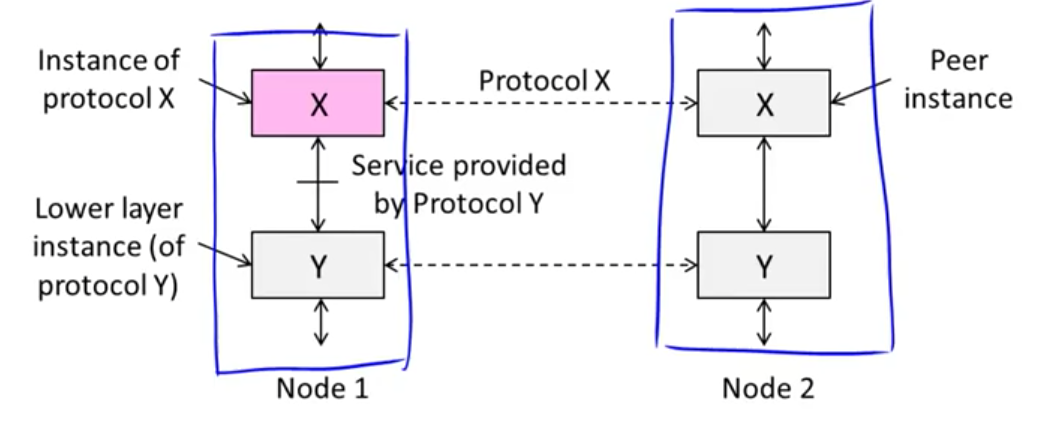
\includegraphics[width=2.2in]{images/1-6-1}
			\caption{Protocols are horizontal, layers are vertical }
			\label{fig:1-6-1}
		\end{minipage}
		\begin{minipage}[t]{0.5\linewidth}
			\centering
			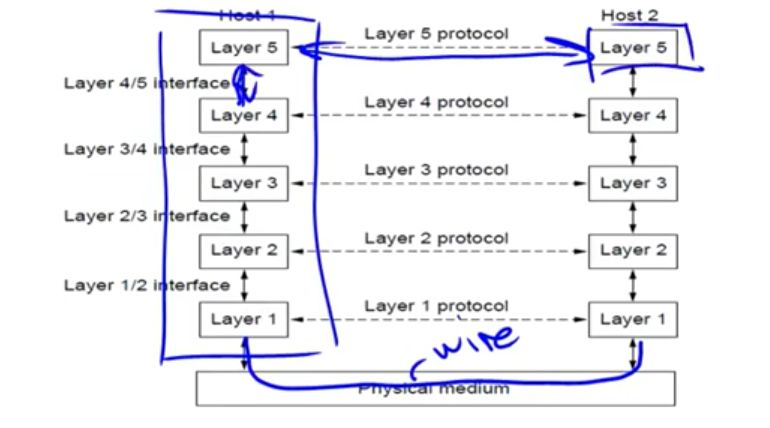
\includegraphics[width=2.2in]{images/1-6-2}
			\caption{protocol stack}
			\label{fig:1-6-2}
		\end{minipage}
	\end{figure}
		
	\begin{itemize}
		\item \underline{Protocols} and \underline{layering} is the main structuring method used to divide up network functionality
		\begin{itemize}
			\item Each instance of a protocol talks virtually to its \underline{peer} using the protocol
			\item Each instance of a protocol uses only the services of the lower layer
		\end{itemize}
		
		\item Protocols are horizontal, layers are vertical, See Figure~\ref{fig:1-6-1}
		\item Set of protocols in use is called a \underline{protocol stack}, See Figure~\ref{fig:1-6-2}
		
		\item Protocols you've probably heard of:
		\begin{itemize}
			\item TCP, IP, 802.11, Ethernet, HTTP, SSL, DNS,..., and many more
		\end{itemize}
		
		\item An example protocol stack
		\begin{itemize}
			\item Used by a web browser on a host that is wirelessly connected to the Internet
		\end{itemize}
	\end{itemize}
	
	\subsection{Encapsulation}
	
	\begin{figure}[h!] % h for here.
	 \centering
	 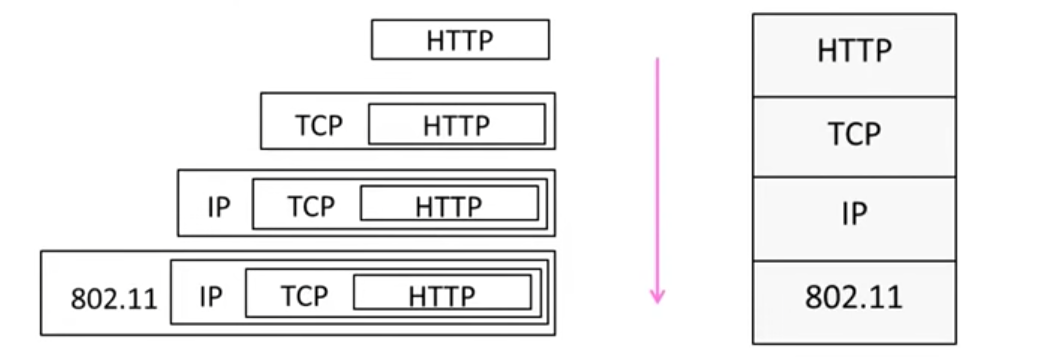
\includegraphics[scale=0.7]{images/1-6-3}
	\caption{ Encapsulation 1 }
	 \label{fig:1-6-3}
	 \end{figure}
	 
	 \begin{figure}[h!] % h for here.
	 \centering
	 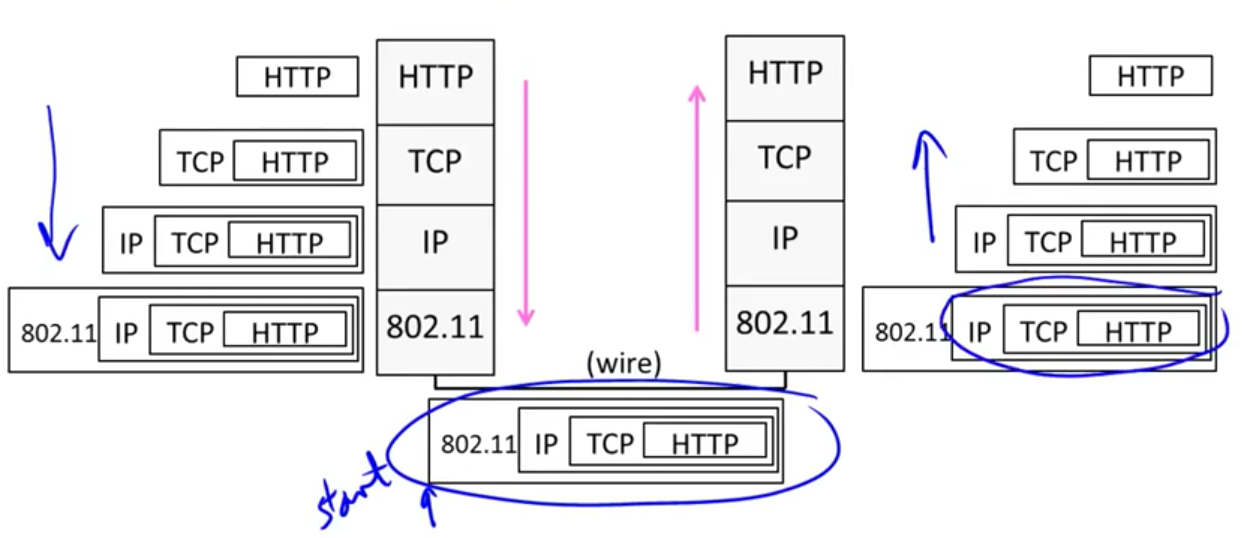
\includegraphics[scale=0.7]{images/1-6-4}
	\caption{ Encapsulation 2 }
	 \label{fig:1-6-4}
	 \end{figure}
	 
	 \begin{figure}[h!] % h for here.
	 \centering
	 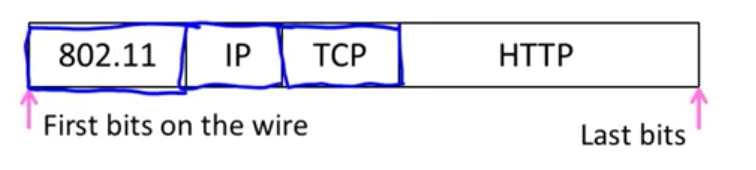
\includegraphics[scale=0.7]{images/1-6-5}
	\caption{ Encapsulation 3 }
	 \label{fig:1-6-5}
	 \end{figure}
	 
	\begin{itemize}
		\item \underline{Encapsulation} is the mechanism used to effect protocol layering
		\begin{itemize}
			\item Lower layer wraps higher layer content, adding its own information to make a new message for delivery
			\item Like sending a letter in an envelope; postal service doesn't look inside
		\end{itemize}
		
		\item Message "on the wire" begins to look an onion, See Figure~\ref{fig:1-6-3}
		\begin{itemize}
			\item Lower layers are outermost
		\end{itemize}
		
		\item See Figure~\ref{fig:1-6-4}
		
		\item Normally draw message like this: See Figure~\ref{fig:1-6-5}
		\begin{itemize}
			\item Each layer adds its own header
		\end{itemize}
		
		\item More involved in practice
		\begin{itemize}
			\item Trailers as well as headers, encrypt/compress contents
			\item Segmentation (divide long message) and reassembly
		\end{itemize}
	\end{itemize}
	
	\subsection{Demultiplexing}
	
	\begin{figure}[h!] % h for here.
	 \centering
	 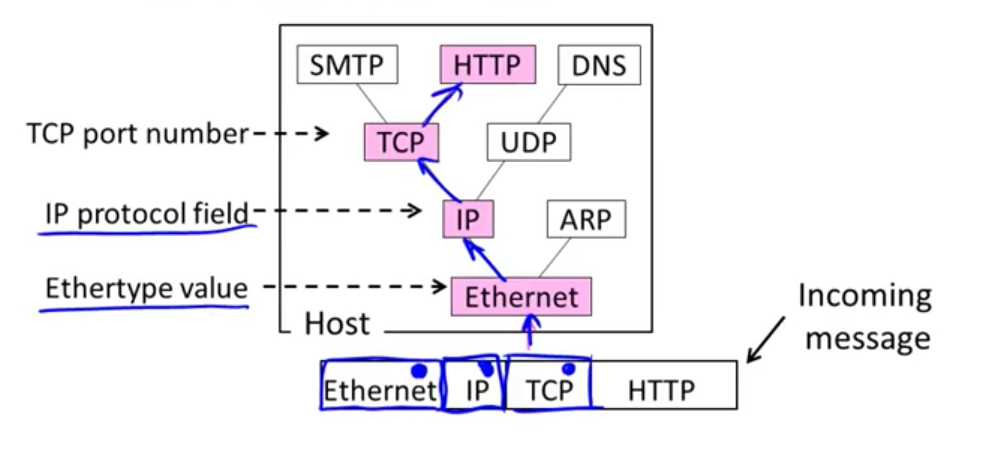
\includegraphics[scale=0.7]{images/1-6-6}
	\caption{ Demultiplexing }
	 \label{fig:1-6-6}
	 \end{figure}
	 
	\begin{itemize}
		\item Done with demultiplexing keys in the headers, See Figure~\ref{fig:1-6-6}
	\end{itemize}
	
	\subsection{Advantage of Layering}
	
	\begin{figure}[h!] % h for here.
	 \centering
	 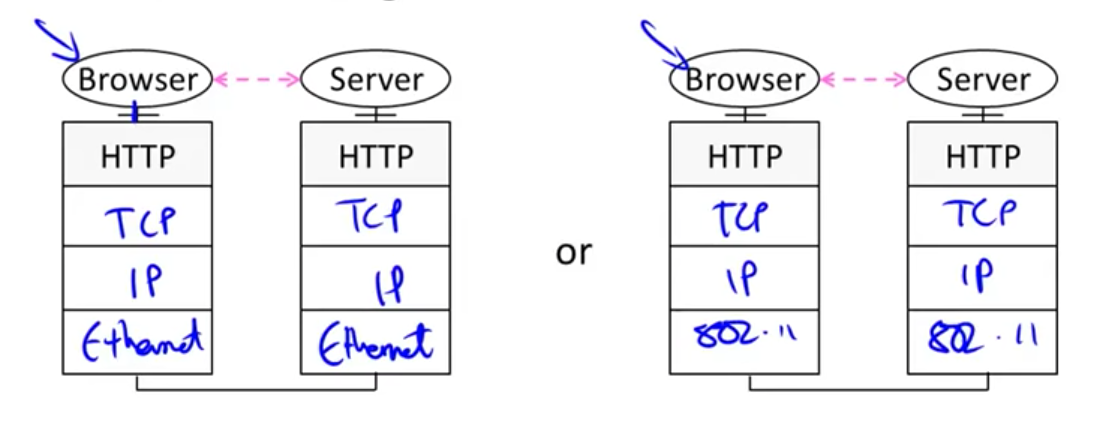
\includegraphics[scale=0.7]{images/1-6-7}
	\caption{ Information hiding and reuse }
	 \label{fig:1-6-7}
	 \end{figure}
	 
	 \begin{figure}[h!] % h for here.
	 \centering
	 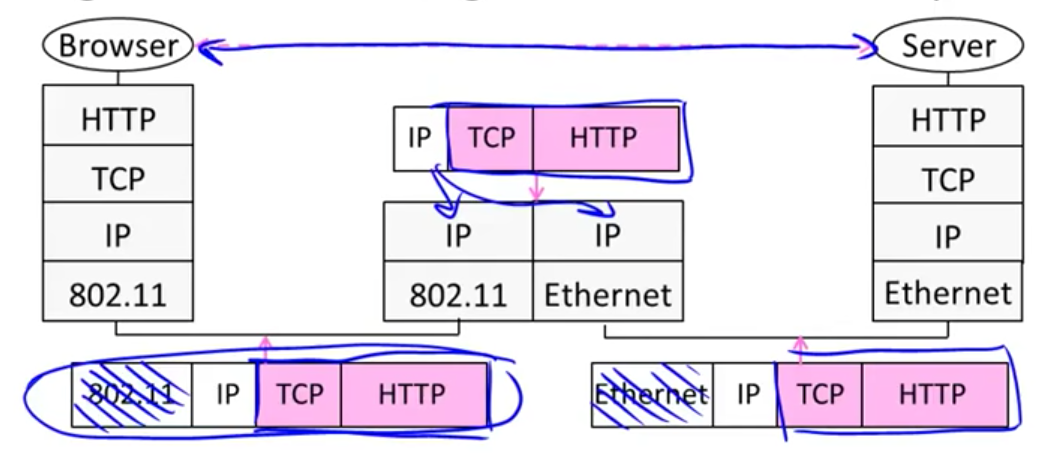
\includegraphics[scale=0.7]{images/1-6-8}
	\caption{ Using information hiding to connect different systems }
	 \label{fig:1-6-8}
	 \end{figure}
	 
	 \begin{itemize}
	 	\item Information hiding and reuse, See Figure~\ref{fig:1-6-7}
	 	
	 	\item Using information hiding to connect different systems, See Figure~\ref{fig:1-6-8}
	 \end{itemize}
	 
	 \subsection{Disadvantage of Layering}
	 \begin{itemize}
	 	\item Adds overhead
	 	\begin{itemize}
	 		\item But minor for long messages
	 	\end{itemize}
	 	
	 	\item Hides information
	 	\begin{itemize}
	 		\item App might care whether it is running over wired or wireless!
	 	\end{itemize}
	 \end{itemize}

\section{Week 1 - Reference Models}
	\subsection{OSI "7 layer" Reference Model}
	
	\begin{figure}[h!] % h for here.
	 \centering
	 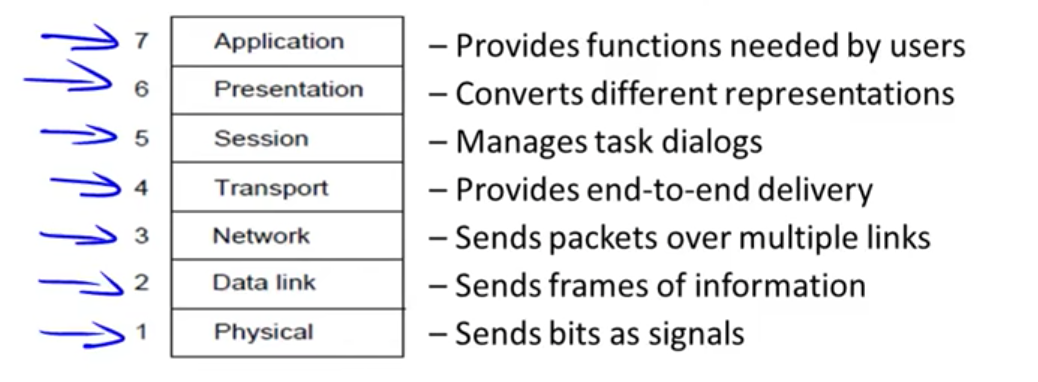
\includegraphics[scale=0.7]{images/1-7-1}
	\caption{ OSI "7 layer" Reference Model }
	 \label{fig:1-7-1}
	 \end{figure}
	 
	\begin{itemize}
		\item A principled, international standard, to connect systems, See Figure~\ref{fig:1-7-1}
		\begin{itemize}
			\item Influential, but not used in practice. (Woops)
		\end{itemize}
	\end{itemize}
	
	\subsection{Internet Reference Model}
	
	\begin{figure}[h!] % h for here.
	 \centering
	 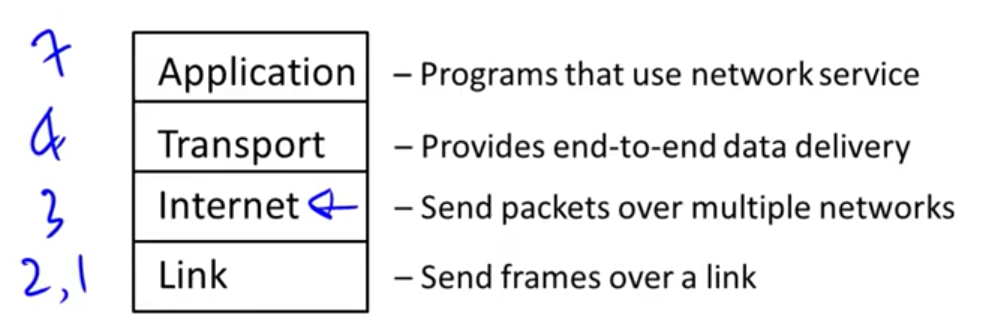
\includegraphics[scale=0.7]{images/1-7-2}
	\caption{ Internet Reference Model}
	 \label{fig:1-7-2}
	 \end{figure}
	 
	 \begin{figure}[h!] % h for here.
	 \centering
	 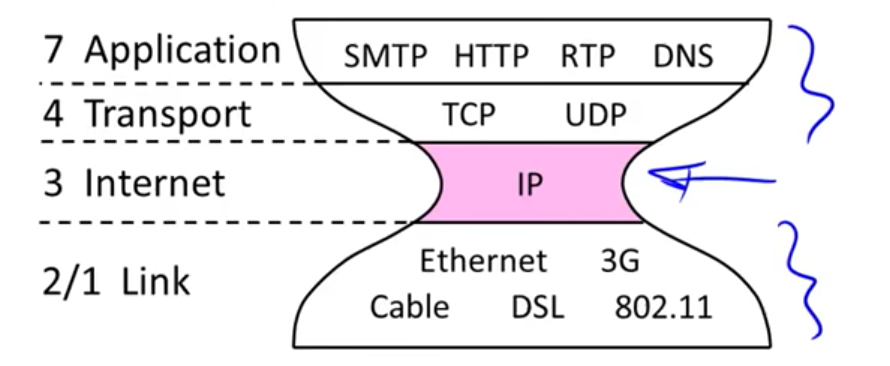
\includegraphics[scale=0.7]{images/1-7-3}
	\caption{ IP is the "narrow waist" of the Internet}
	 \label{fig:1-7-3}
	 \end{figure}
	 
	\begin{itemize}
		\item A four layer model based on experience; omits some OSI layers and uses IP as the network layer. See Figure~\ref{fig:1-7-2}
		
		\item IP is the "narrow waist" of the Internet, See Figure~\ref{fig:1-7-3}
		\begin{itemize}
			\item Supports many different links below and apps above
		\end{itemize}
	\end{itemize}
	
	\subsection{Standards Bodies}
	
	 \begin{figure}[h!] % h for here.
	 \centering
	 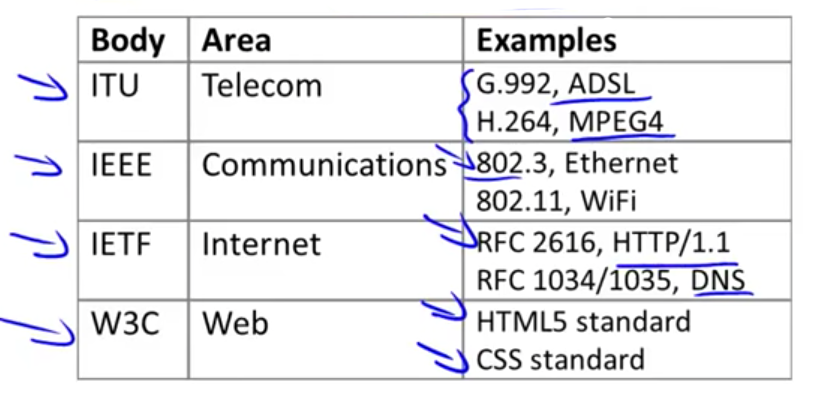
\includegraphics[scale=0.7]{images/1-7-4}
	\caption{ Standards Bodies}
	 \label{fig:1-7-4}
	 \end{figure}
	 
	 \begin{itemize}
	 	\item Where all the protocols come from! See Figure~\ref{fig:1-7-4}
	 	\begin{itemize}
	 		\item Focus is on interoperability
	 	\end{itemize}
	 \end{itemize}
	 
	 \subsection{Layer-based Names}
	 
	 \begin{figure}[h!] % h for here.
	 \centering
	 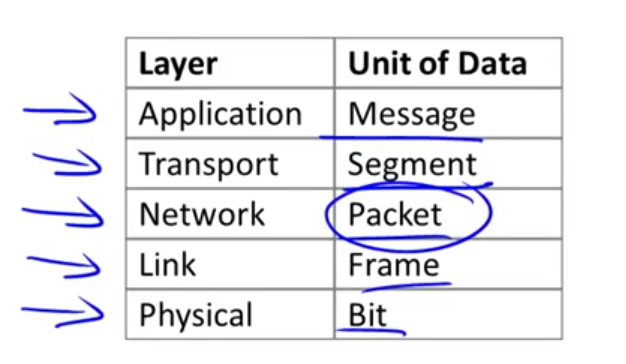
\includegraphics[scale=0.7]{images/1-7-5}
	\caption{ Units of data}
	 \label{fig:1-7-5}
	 \end{figure}
	 
	  %\begin{% figure 1 & 2
	\begin{figure}
		\begin{minipage}[t]{0.5\linewidth}
			\centering
			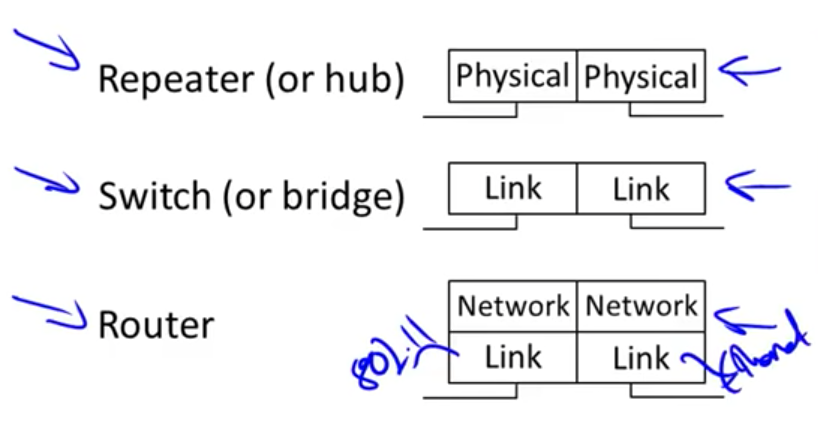
\includegraphics[width=2.2in]{images/1-7-6}
			\caption{Devices in the network  1}
			\label{fig:1-7-6}
		\end{minipage}
		\begin{minipage}[t]{0.5\linewidth}
			\centering
			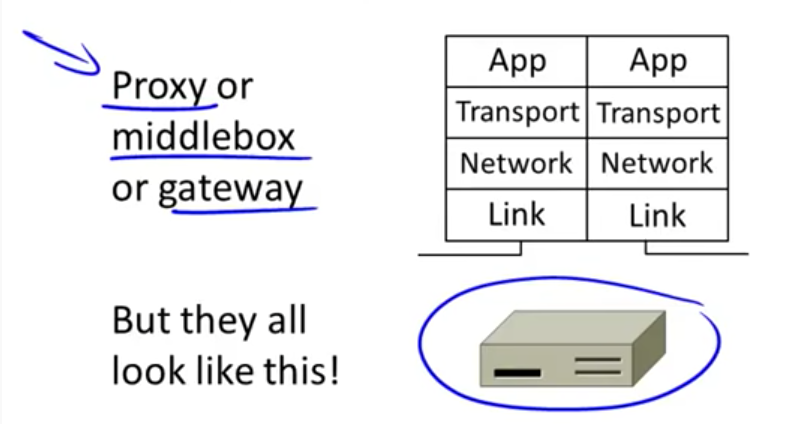
\includegraphics[width=2.2in]{images/1-7-7}
			\caption{devices in the network 2}
			\label{fig:1-7-7}
		\end{minipage}
	\end{figure}
	 
	 \begin{itemize}
	 	\item For units of data: See Figure~\ref{fig:1-7-5}
	 	
	 	\item For devices in the network: See Figure~\ref{fig:1-7-6} and Figure~\ref{fig:1-7-7}
	 \end{itemize}
	 
\section{Week 1 - Internet History}	
	略
\section{Week 1 - Lecture Outline}
	\subsection{Textbook}
	\begin{itemize}
		\item "Computer Networks" 5/E (US or Intl, print or e-text) is optional but recommended
		\begin{itemize}
			\item We'll do our best to let you work without it (with the odd web search)
			\item Read it for explanations, greater depth, extra topics, a reference, etc.
		\end{itemize}
	\end{itemize}
	
	
\section{Week 2 - Physical Layer Overview}
	\subsection{Scope of the Physical Layer}
	
	\begin{figure}[h!] % h for here.
	 \centering
	 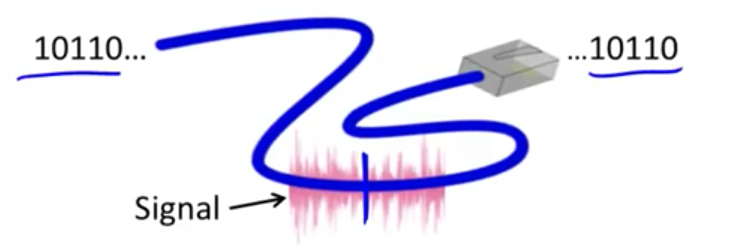
\includegraphics[scale=0.7]{images/2-1-1}
	\caption{ Transfer message bits over a link}
	 \label{fig:2-1-1}
	 \end{figure}
	 
	\begin{itemize}
		\item Concerns how signals are used to transfer message bits over a link, See Figure~\ref{fig:2-1-1}
		\begin{itemize}
			\item Wires etc. carry \underline{analog signals}
			\item We want to send \underline{digital bits}
		\end{itemize}
	\end{itemize}
	
	\subsection{Topics}
	\begin{itemize}
		\item {\color{blue} 1.} Properties of media
		\begin{itemize}
			\item Wires, fiber optics, wireless
		\end{itemize}
		
		\item {\color{blue} 2.} Simple signal propagation
		\begin{itemize}
			\item	Bandwidth, attenuation, noise
		\end{itemize}
		
		\item {\color{blue} 3.} Modulation Schemes
		\begin{itemize}
			\item Representing bits, noise
		\end{itemize}
		
		\item {\color{blue} 4.} Fundamental limits
		\begin{itemize}
			\item Nyquist, Shannon
		\end{itemize}
	\end{itemize}
	
	\subsection{Simple Link Model}
	
	\begin{figure}[h!] % h for here.
	 \centering
	 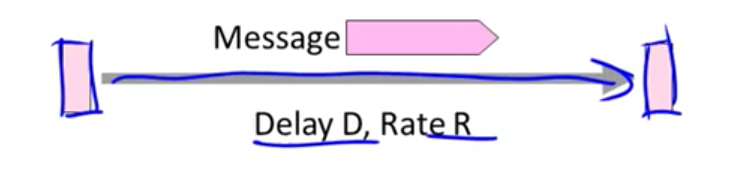
\includegraphics[scale=0.7]{images/2-1-2}
	\caption{ Simple Link Model}
	 \label{fig:2-1-2}
	 \end{figure}
	 
	\begin{itemize}
		\item We'll end with an abstraction of a physical channel , See Figure~\ref{fig:2-1-2}
		\begin{itemize}
			\item \underline{Rate} (or bandwidth, capacity, speed) in bits/second
			\item \underline{Delay} in seconds, related to length
		\end{itemize}
		
		\item Other important properties:
		\begin{itemize}
			\item Whether the channel is broadcast, and its error rate
		\end{itemize}
	\end{itemize}
	
	\subsection{Message Latency}
	\begin{itemize}
		\item \underline{Latency} is the delay to send a message over a link
		\begin{itemize}
			\item \underline{Transmission delay:} time to put M-bit message "on the wire" \\
			$$
			T-delay = M \, (bits) / Rate \, (bits/sec) = M/R \, seconds
			$$
			
			\item \underline{Propagation delay:} time for bits to propagate across the wire \\
			$$
			P-delay = Length /speed \, of \, signals = \frac{Length}{\frac{2}{3} C} = D \, seconds 
			$$			
			
			\item Combining the two terms we have: $L = M/R + D$
		\end{itemize}
		
	\end{itemize}
	
	\subsection{Metric Units}
	
	%%% 开始表格
		\begin{table}[h] 
		\begin{center}
		\begin{tabular}{p{2cm} | p{1cm} | p{3cm} | p{2cm}} 
		\hline
		\hline
		Prefix & Exp. & prefix & exp. \\
		\hline 
		K(ilo) & $10^3$ & m(illi) 毫秒 & $10^{-3}$\\
		\hline
		 M(ega) & $10^6$ & $\mu$(micro) 微秒 & $10^{-6}$\\
		\hline
		G(iga) & $10^9$ & n(ano) & $10^{-9}$\\
		\hline
		\hline
		\end{tabular}
		\end{center}
		\caption{Socket API Functions} 
		\label{table:2-1-1}
		\end{table}
		%%% 结束表格
		
	\begin{itemize}
		\item The main prefixes we use:  See Table~\ref{table:2-1-1}
		\item Use powers of 10 for rates, 2 for storage
		\begin{itemize}
			\item 1 Mbps = 1,000,000 bps, 1 KB = $2^{10}$ bytes
		\end{itemize}
		
		\item "B" is for bytes, "b" is for bits
	\end{itemize}

	\subsection{Latency Example}
	\begin{itemize}
		\item "Dialup" with a telephone modem:
		\begin{equation}
		\begin{split}
		& D = 5 \; ms, R= 56 \; Kbps, M = 1250 \; bytes \\
		& L  = 5 \; ms + (1250 \times 8) / (56 \times 10^3) \; sec = 148 \; ms!
		\end{split}
		\end{equation}
		
		\item Broadband cross-country link:
		\begin{equation}
		\begin{split}
		& D= 50 \; ms, R= 10 \; Mbps, M= 1250 \; bytes \\
		& L =50 \; ms + (1250 \times 8) / (10 \times 10^6) \; sec = 51 ms
		\end{split}
		\end{equation}
		
		\item A long link or a slow rate means high latency
		\begin{itemize}
			\item Often, one delay component dominates
		\end{itemize}
	\end{itemize}
	
	\subsection{Bandwidth-Delay Product}
	\begin{itemize}
		\item Messages take space on the wire!
		\item The amount of data in flight is the \underline{bandwidth-delay (BD) product}
		$$
		BD = R \times D
		$$
		\begin{itemize}
			\item Measure in bits, or in messages
			\item Small for LANs, big for "long fat" pipes
			\item 表示第一个包到达接收端的时候,发送端总共发送进入网络的数据量,单位用bit表示。
		\end{itemize}
	\end{itemize}
	

\section{Week 2 - Media}
	\subsection{Types of Media}
	\begin{itemize}
		\item \underline{Media} propagate \underline{signals} that carry \underline{bits} of information
		\item We'll look at some common types:
		\begin{itemize}
			\item Wires
			\item Fiber (fiber optic cables)
			\item Wireless
		\end{itemize}
	\end{itemize}
	
	\subsection{Wires - Twisted Pair}
	
	\begin{figure}[h!] % h for here.
	 \centering
	 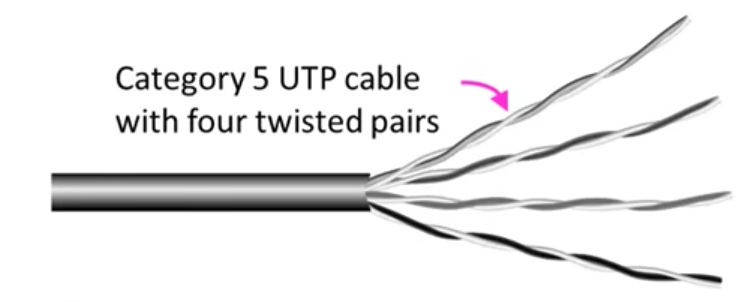
\includegraphics[scale=0.7]{images/2-2-1}
	\caption{ Wires - Twisted Pair}
	 \label{fig:2-2-1}
	 \end{figure}
	 
	\begin{itemize}
		\item Very common; used in LANs and telephone lines, Figure~\ref{fig:2-2-1}
		\begin{itemize}
			\item Twists reduce radiated signal
		\end{itemize}
	\end{itemize}
	
	\subsection{Wires - Coaxial Cable 同轴电缆}
	
	\begin{figure}[h!] % h for here.
	 \centering
	 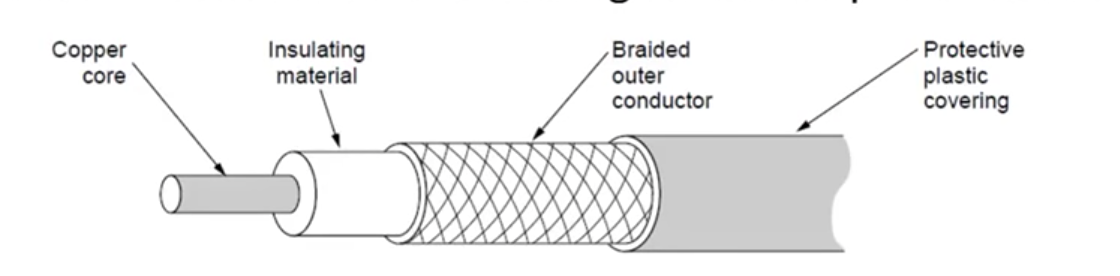
\includegraphics[scale=0.7]{images/2-2-2}
	\caption{ Wires - Coaxial Cable}
	 \label{fig:2-2-2}
	 \end{figure}
	 
	\begin{itemize}
		\item Also common. better shielding for better performance, See Figure~\ref{fig:2-2-2}
		\item Other kinds of wires too: e.g., electrical power (§2.2.4)
	\end{itemize}
	
	\subsection{Fiber}
	
	\begin{figure}[h!] % h for here.
	 \centering
	 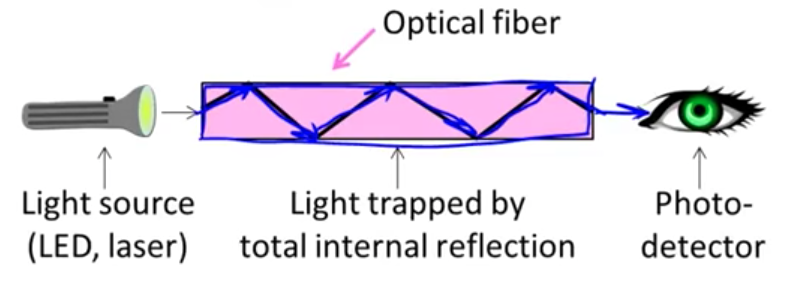
\includegraphics[scale=0.7]{images/2-2-3}
	\caption{ Fiber}
	 \label{fig:2-2-3}
	 \end{figure}
	 
	 \begin{figure}[h!] % h for here.
	 \centering
	 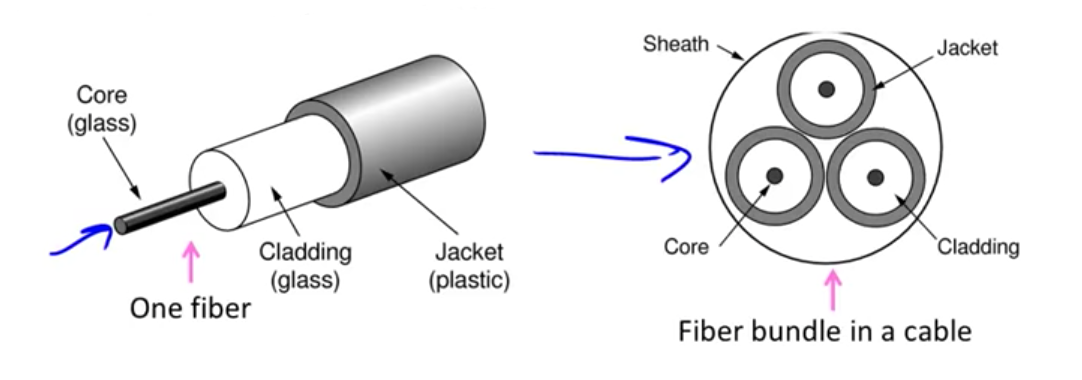
\includegraphics[scale=0.7]{images/2-2-4}
	\caption{ Fiber 2}
	 \label{fig:2-2-4}
	 \end{figure}
	 
	\begin{itemize}
		\item Long, thin, pure strands of glass, See Figure~\ref{fig:2-2-3}
		\begin{itemize}
			\item Enormous bandwidth (high speed) over long distances
		\end{itemize}
		
		\item Two varieties: multi-mode (shorter links, cheaper) and single-mode (up to ~100 km), See Figure~\ref{fig:2-2-4}
	\end{itemize}
	
	\subsection{Wireless}
	
	\begin{figure}[h!] % h for here.
	 \centering
	 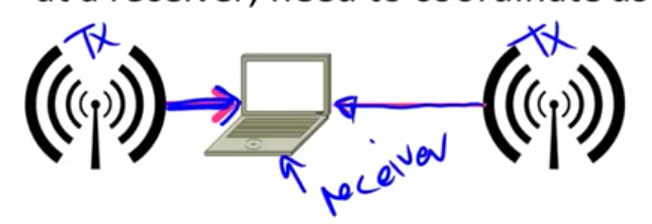
\includegraphics[scale=0.7]{images/2-2-5}
	\caption{ Wireless}
	 \label{fig:2-2-5}
	 \end{figure}
	 
	 \begin{figure}[h!] % h for here.
	 \centering
	 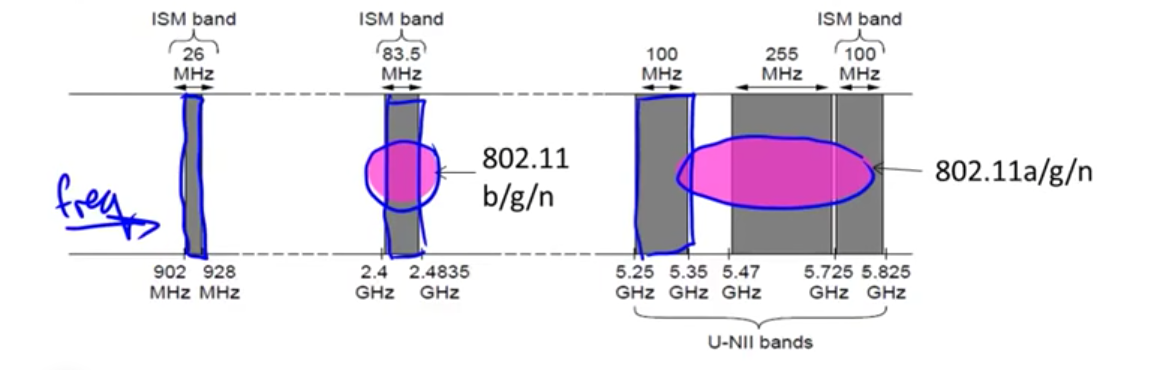
\includegraphics[scale=0.7]{images/2-2-6}
	\caption{ Wireless 2}
	 \label{fig:2-2-6}
	 \end{figure}
	 
	 \begin{itemize}
	 	\item	Sender radiates signal over a region, See Figure~\ref{fig:2-2-5}
	 	\begin{itemize}
	 		\item In many directions, unlike a wire, to potentially many receivers
	 		\item Nearby signal (same freq.) \underline{interface} at a receiver; need to coordinate use
	 	\end{itemize}
	 	
	 	\item Microwave, e.g., 3G, and unlicensed (ISM) frequencies, e.g., WiFi, are widely used for computer networking, See Figure~\ref{fig:2-2-6}
	 \end{itemize}

\section{Week 2 - Signals}
	\subsection{Topic}
	
	 \begin{figure}[h!] % h for here.
	 \centering
	 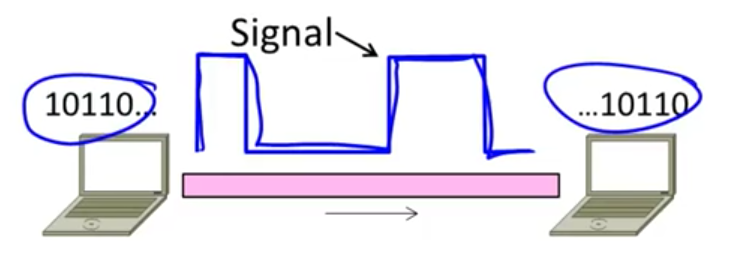
\includegraphics[scale=0.7]{images/2-3-1}
	\caption{ Topic of signals}
	 \label{fig:2-3-1}
	 \end{figure}
	 
	\begin{itemize}
		\item Analog signals encode digital bits. We want to know what happens as signals \underline{propagate} over media, See Figure~\ref{fig:2-3-1}
	\end{itemize}
	
	\subsection{Frequency Representation}
	
	 \begin{figure}[h!] % h for here.
	 \centering
	 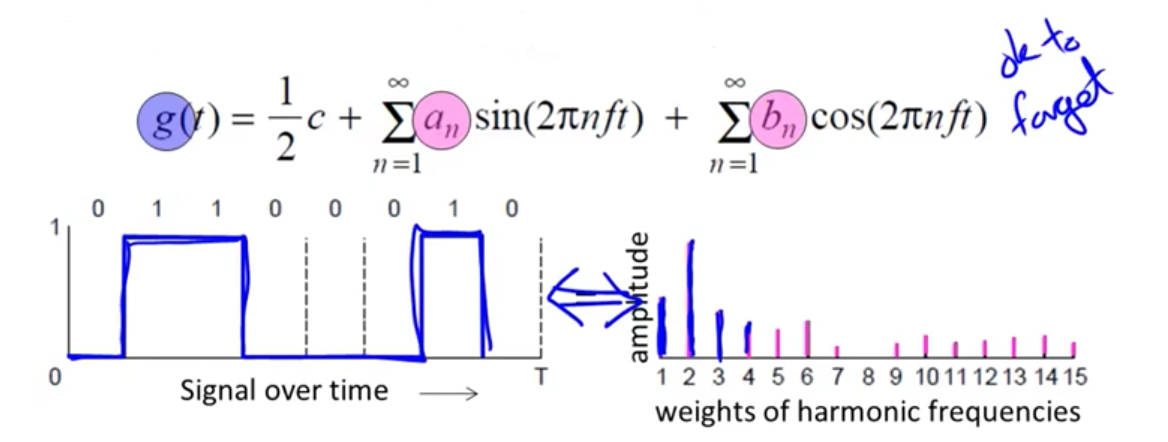
\includegraphics[scale=0.7]{images/2-3-2}
	\caption{ Frequency Representation}
	 \label{fig:2-3-2}
	 \end{figure}
	 
	\begin{itemize}
		\item A signal over time can be represented by its frequency components (called Fourier analysis) , See Figure~\ref{fig:2-3-2}
	\end{itemize}
	
	\subsection{Effect of Less Bandwidth}
	\begin{figure}[h!] % h for here.
	 \centering
	 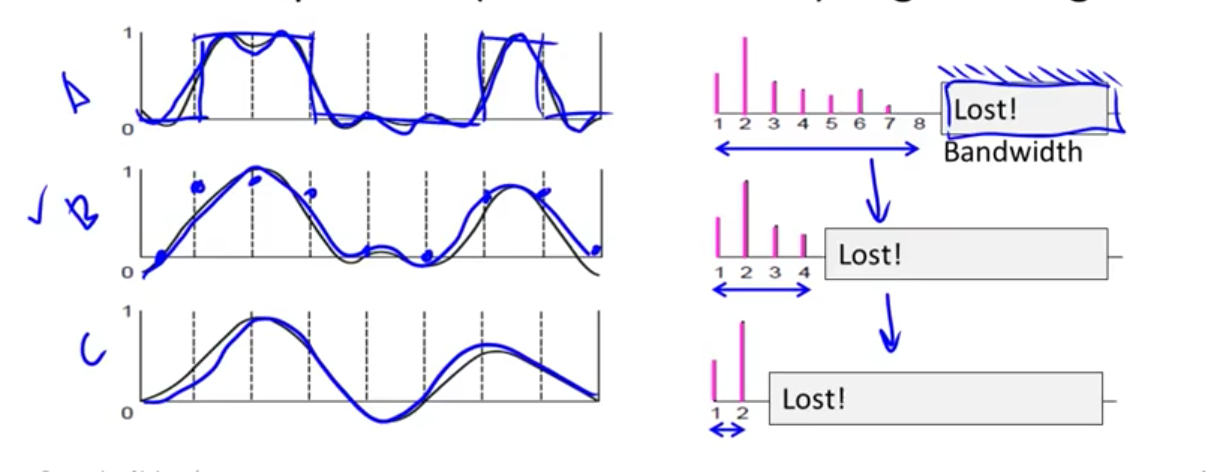
\includegraphics[scale=0.7]{images/2-3-3}
	\caption{ Effect of Less Bandwidth}
	 \label{fig:2-3-3}
	 \end{figure}
	 
	 \begin{itemize}
	 	\item Fewer frequencies (=less bandwidth) degrades signal, See Figure~\ref{fig:2-3-3}
	 \end{itemize}
	 
	 \subsection{Signals over a Wire}
	 
	 \begin{figure}[h!] % h for here.
	 \centering
	 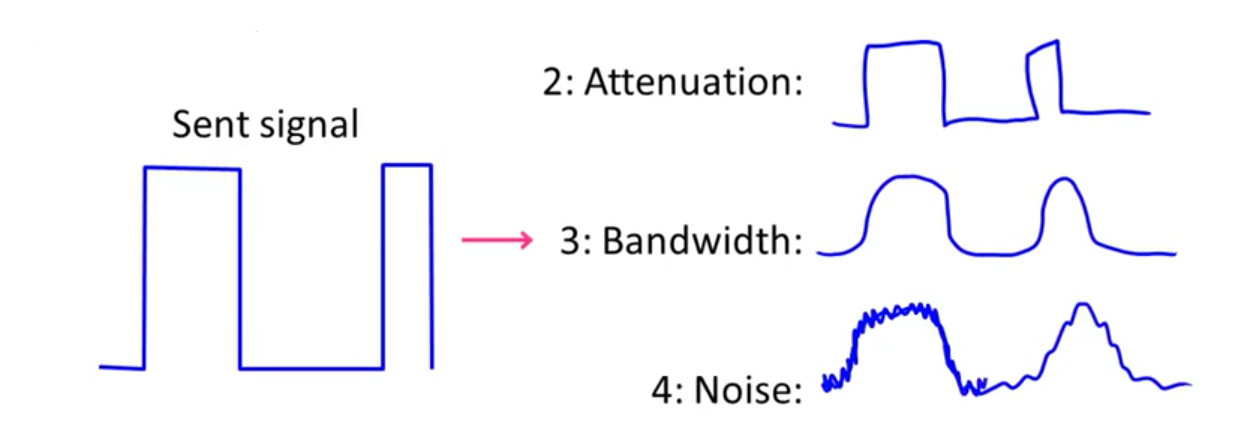
\includegraphics[scale=0.7]{images/2-3-4}
	\caption{ Signals over a Wire}
	 \label{fig:2-3-4}
	 \end{figure}
	 
	 \begin{itemize}
	 	\item What happens to a signal as it passed over a wire?
	 	\begin{itemize}
	 		\item {\color{blue} 1.} The signal is delayed (propagates at $\frac{2}{3} C$)
	 		\item {\color{blue} 2.} The signal is attenuated (goes for m to km)
	 		\item {\color{blue} 3.} Frequencies above a cutoff are highly attenuated
	 		\item {\color{blue} 4.} Noise is added to the signal (later, causes errors)
	 	\end{itemize}
	 	
	 	\item Example See Figure~\ref{fig:2-3-4}
	 	
	 	\item Tips:
	 	\begin{itemize}
	 		\item EE: Bandwidth = width of frequency band, measured in Hz
	 		\item CS: Bandwidth = information carrying capacity, in bits/sec
	 	\end{itemize}
	 \end{itemize}
	 
	 \subsection{Signals over Fiber}
	 
	 \begin{figure}[h!] % h for here.
	 \centering
	 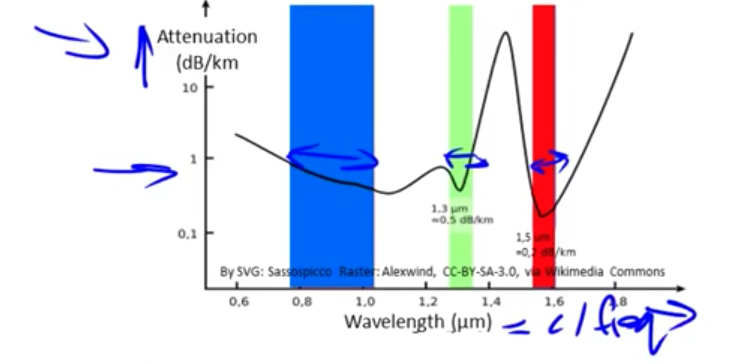
\includegraphics[scale=0.7]{images/2-3-5}
	\caption{ Signals over Fiber}
	 \label{fig:2-3-5}
	 \end{figure}
	 
	 \begin{itemize}
	 	\item Light propagates with very low loss in three very wide frequency bands, See Figure~\ref{fig:2-3-5}
	 	\begin{itemize}
	 		\item Use a carrier to send information
	 	\end{itemize}
	 \end{itemize}
	 
	 \subsection{Signals over Wireless}
	 
	 %% 四幅图 1 & 2 & 3 & 4
	\begin{figure}
		\centering
		\subfigure[Signals transmitted on a carrier frequency]{
			\begin{minipage}[b]{0.4\textwidth}
				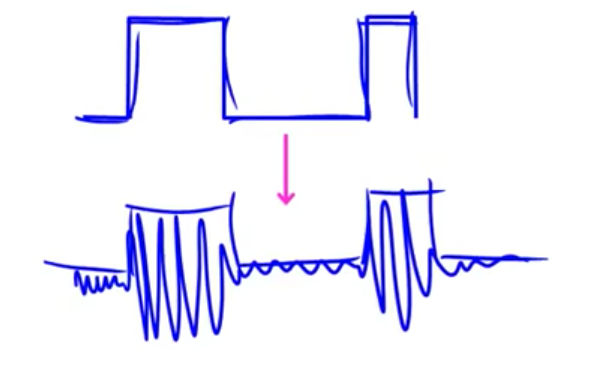
\includegraphics[width=1\textwidth]{images/2-3-6} 
			\end{minipage}
			\label{fig:2-3-6}
		}
	    	\subfigure[Attenuate ]{
	    		\begin{minipage}[b]{0.4\textwidth}
	   		 	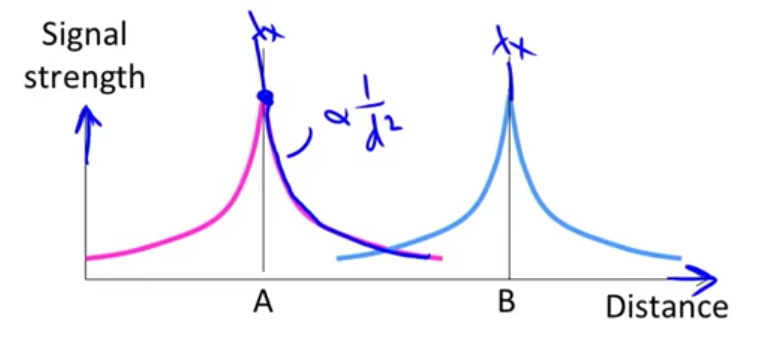
\includegraphics[width=1\textwidth]{images/2-3-7}
	    		\end{minipage}
			\label{fig:2-3-7}
	    	}
		\\ 
		\subfigure[ Interfere ]{
			\begin{minipage}[b]{0.4\textwidth}
				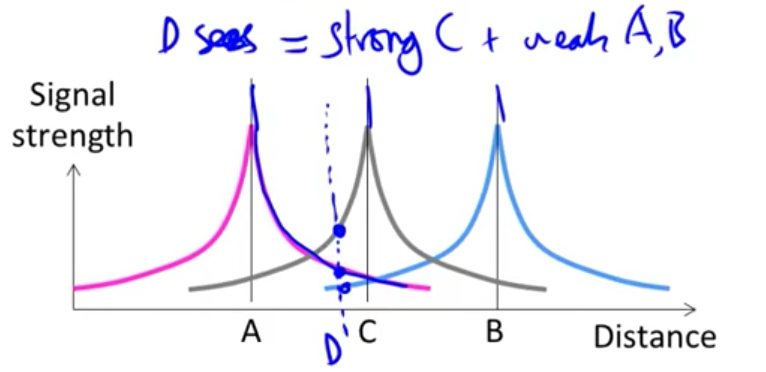
\includegraphics[width=1\textwidth]{images/2-3-8} 
			\end{minipage}
			\label{fig:2-3-8}
		}
	    	\subfigure[Spatial reuse]{
	    		\begin{minipage}[b]{0.4\textwidth}
			 	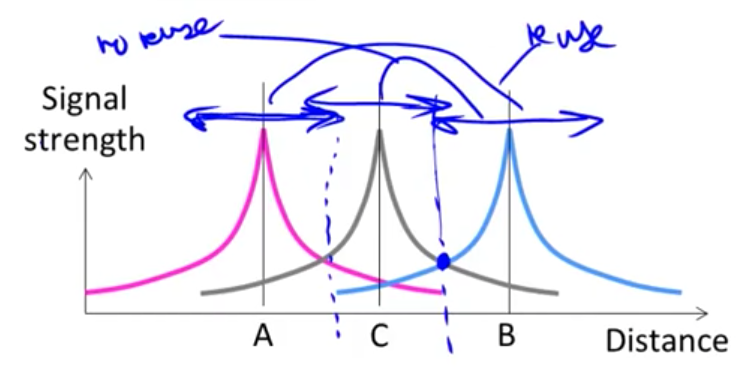
\includegraphics[width=1\textwidth]{images/2-3-9}
	    		\end{minipage}
			\label{fig:2-3-9}
	    	}
		\caption{Four Figures}
	\end{figure}
	%% 结束四幅图
	
	 \begin{itemize}
	 	\item Signals transmitted on a carrier frequency, like fiber (more later) , See Figure~\ref{fig:2-3-6}
	 	\item Travel at speed of light, spread out and attenuate faster than $\frac{1}{dist ^ 2}$ , See Figure~\ref{fig:2-3-7}
	 	\item Multiple signals on the same frequency interfere at a receiver, See Figure~\ref{fig:2-3-8}
	 	\item Interference leads to notion of \underline{spatial reuse} (of same freq.), See Figure~\ref{fig:2-3-9}
	 	
	 	\item Various other effects too!
	 	\begin{itemize}
	 		\item Wireless propagation is complex, depends on environment
	 	\end{itemize}
	 	
	 	\item Some key effects are highly frequency dependent,
	 	\begin{itemize}
	 		\item E.g., \underline{multipath} at microwave frequencies
	 	\end{itemize}
	 	
	 \end{itemize}
	 
	 \subsection{Wireless Multipath}
	 
	 \begin{figure}[h!] % h for here.
	 \centering
	 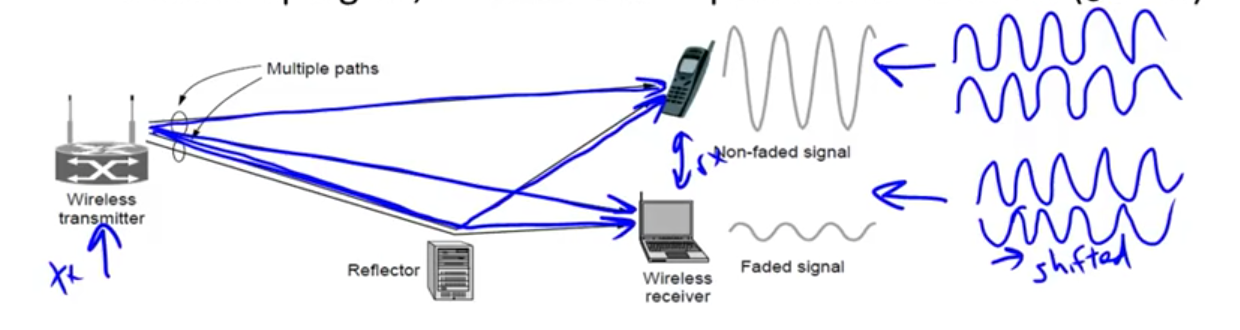
\includegraphics[scale=0.7]{images/2-3-10}
	\caption{ Wireless Multipath}
	 \label{fig:2-3-10}
	 \end{figure}
	 
	 \begin{itemize}
	 	\item Signals bounce off objects and take multiple paths, See Figure~\ref{fig:2-3-10}
	 	\begin{itemize}
	 		\item Some frequencies attenuated at receiver, varies with location
	 		\item Messes up signal; handled with sophisticated method (§2.5.3)
	 	\end{itemize}
	 \end{itemize}
	 
\section{Week 2 - Modulation}
	\subsection{Topic of Modulation}
	 \begin{figure}[h!] % h for here.
	 \centering
	 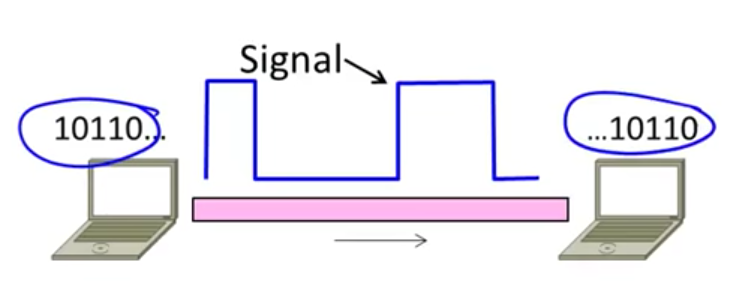
\includegraphics[scale=0.7]{images/2-4-1}
	\caption{ Topic of Modulation}
	 \label{fig:2-4-1}
	 \end{figure}
	 
	 \begin{itemize}
	 	\item We've talked about signals representing bits. How, exactly? See Figure~\ref{fig:2-4-1}
	 	\begin{itemize}
	 		\item This is the topic of \underline{modulation}
	 	\end{itemize}
	 \end{itemize}
	 
	 \subsection{A Simple Modulation}
	 \begin{figure}[h!] % h for here.
	 \centering
	 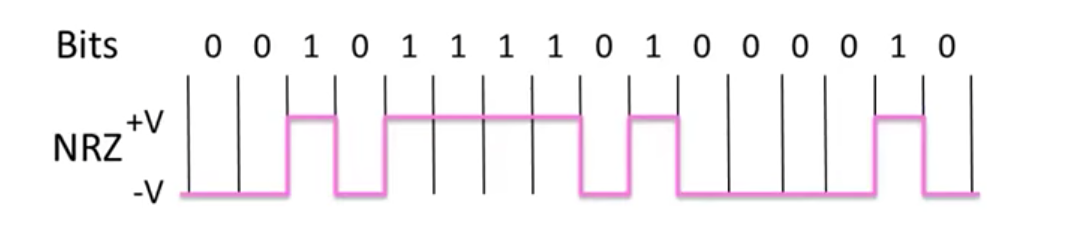
\includegraphics[scale=0.7]{images/2-4-2}
	\caption{ A Simple Modulation}
	 \label{fig:2-4-2}
	 \end{figure}
	 
	 \begin{itemize}
	 	\item Let a high voltage (+V) represent a 1, and low voltage (-V) represent a 0, See Figure~\ref{fig:2-4-2}
	 	\begin{itemize}
	 		\item This is called NRZ (Non-Return to Zero)
	 	\end{itemize}
	 \end{itemize}
	 
	 \subsection{Many Other Schemes}
	 \begin{figure}[h!] % h for here.
	 \centering
	 \includegraphics[scale=0.7]{images/2-4-3}
	\caption{ Many Other Schemes}
	 \label{fig:2-4-3}
	 \end{figure}
	 
	 \begin{itemize}
	 	\item Can use more signal levels, e.g., 4 levels in 2 bits per \underline{symbol}, See Figure~\ref{fig:2-4-3}
	 	\item Practical schemes are driven by engineering considerations
	 	\begin{itemize}
	 		\item E.g., clock recovery
	 	\end{itemize}
	 \end{itemize}
	 
	 \subsection{Clock Recovery}
	 \begin{figure}[h!] % h for here.
	 \centering
	 \includegraphics[scale=0.7]{images/2-4-4}
	\caption{ Clock Recovery}
	 \label{fig:2-4-4}
	 \end{figure}
	 
	 \begin{itemize}
	 	\item Um, how may zeros was that? See Figure~\ref{fig:2-4-4}
	 	\begin{itemize}
	 		\item Receiver needs frequent signal transitions to decode bits
	 	\end{itemize}
	 	
	 	\item Several possible designs
	 	\begin{itemize}
	 		\item E.g.,. Manchester coding and scrambling (§2.5.1)
	 	\end{itemize}
	 \end{itemize}
	
	 \subsection{Clock  Recovery - 4B/5B}
	 \begin{itemize}
	 	\item Map every 4 data bits into 5 code bits without long runs of zeros
	 	\begin{itemize}
	 		\item 0000 $ \rightarrow$ 11110, 0001 $\rightarrow$ 01001, \\
	 				1110 $ \rightarrow$ 11100, ... 1111 $\rightarrow$ 11101 
	 		\item Has at most 3 zeros in a row
	 		\item Also invert signal level on a 1 to break up long runs of 1s (called NRZI, §2.5.1) \underline{NRZI中的I是invert}
	 	\end{itemize}
	 	
	 	\item Message bits: 1 1 1 1 0 0 0 0 0 0 0 1   , See Figure~\ref{fig:2-4-5} \\
	 	1 变 0 不变
	 	\begin{figure}[h!] % h for here.
		 \centering
		 \includegraphics[scale=0.7]{images/2-4-5}
		\caption{ Message bits: 1 1 1 1 0 0 0 0 0 0 0 1}
		 \label{fig:2-4-5}
		 \end{figure}
	 \end{itemize}
	 
	 \subsection{Passband Modulation}
	 \begin{itemize}
	 	\item What we have seen so far is \underline{baseband} modulation for wires
	 	\begin{itemize}
	 		\item Signal is sent directly on a wire
	 	\end{itemize}
	 	
	 	\item These signals do not propagate well on fiber / wireless
	 	\begin{itemize}
	 		\item Need to send at higher frequencies
	 	\end{itemize}
	 	
	 	\item \underline{Passband} modulation carries a signal by modulating a carrier
	 	
	 	\item Carrier is simply a signal oscillating at a desired frequency: See Figure~\ref{fig:2-4-6}
	 	\begin{figure}[h!] % h for here.
		 \centering
		 \includegraphics[scale=0.7]{images/2-4-6}
		\caption{ Carrier}
		 \label{fig:2-4-6}
		 \end{figure}
		 
		 \item We can modulate it by changing:
		 \begin{itemize}
		 	\item Amplitude, frequency, or phase, See Figure~\ref{fig:2-4-7}
		 \end{itemize}
		 
		 \begin{figure}[h!] % h for here.
		 \centering
		 \includegraphics[scale=0.7]{images/2-4-7}
		\caption{ Modulate it by changing Amplitude, frequency, or phase}
		 \label{fig:2-4-7}
		 \end{figure}
	 \end{itemize}
	 
\section{Week 2 - Limits}
	\subsection{Topic of Limits}
	\begin{itemize}
		\item How rapidly can we send information over a link?
		\begin{itemize}
			\item \underline{Nyquist} limit (~1924)
			\item \underline{Shannon} capacity (1948)
		\end{itemize}
		
		\item Practical systems are devised to approach these limits
	\end{itemize}
	
	\subsection{Key Channel Properties}
	\begin{itemize}
		\item The bandwidth (B), signal strength (S), and noise strength (N), See Figure~\ref{fig:2-5-1}
		\begin{itemize}
			\item B limits the rate of transitions
			\item S and N limit how many signal levels we can distinguish
		\end{itemize}
		
		 \begin{figure}[h!] % h for here.
		 \centering
		 \includegraphics[scale=0.7]{images/2-5-1}
		\caption{ Key Channel Properties}
		 \label{fig:2-5-1}
		 \end{figure}
	\end{itemize}
	
	\subsection{Nyquist Limit}
	\begin{itemize}
		\item The maximum \underline{symbol} rate is 2B , See Figure~\ref{fig:2-5-2}
		 \begin{figure}[h!] % h for here.
		 \centering
		 \includegraphics[scale=0.7]{images/2-5-2}
		\caption{ Nyquist Limit}
		 \label{fig:2-5-2}
		 \end{figure}
		 
		 \item Thus if there are V signal levels, ignoring noise, the maximum bit rate is: $R = 2B\, \log_2 V \; bits/sec$
	\end{itemize}
	
	\subsection{Shannon Capacity}
	
	\begin{figure}[h!] % h for here.
	 \centering
	 \includegraphics[scale=0.7]{images/2-5-3}
	\caption{ Shannon Capacity}
	 \label{fig:2-5-3}
	 \end{figure}
	
	\begin{itemize}
		\item How many levels we can distinguish depends on S/N, See Figure~\ref{fig:2-5-3}
		\begin{itemize}
			\item Or SNR, the \underline{Signal-to-Noise Ratio}
			\item Note noise is random, hence some errors
		\end{itemize}
		
		\item SNR given on a log-scale in deciBels:
		\begin{itemize}
			\item $SNR_{dB} = 10\log_{10} (S/N)$
		\end{itemize}
		
		\item Shannon limit is for capacity (C), the maximum information carrying rate of the channel: $ C = B \, \log_2 (1+S/N) \; bits/sec $
	\end{itemize}
	
	\subsection{Wired/Wireless Perspective}
	\begin{itemize}
		\item Wires, and Fiber         {\color{red} ( Engineer SNR for data rate)}
		\begin{itemize}
			\item Engineer link to have requisite SNR and B $\rightarrow$ Can fix data rate
		\end{itemize}
		
		\item Wireless        {\color{red}   ( Adapt data rate to SNR )}
		\begin{itemize}
			\item Given B, but SNR varies greatly, e.g., up to 60 dB! $\rightarrow$ Can't design for worst case, must adapt data rate
		\end{itemize}
	\end{itemize}
	
	\subsection{Putting it all together - DSL}
	\begin{itemize}
		\item DSL (Digital Subscriber Line, see §2.6.3) is widely used for broadband; many variants offer 10s of Mbps , See Figure~\ref{fig:2-5-4}
		\begin{itemize}
			\item Reuse twisted pair telephone line to the home; it has up to ~2MHz of bandwidth but uses only the lowest ~4kHz
		\end{itemize}
			
		\begin{figure}[h!] % h for here.
		\centering
		 \includegraphics[scale=0.7]{images/2-5-4}
		\caption{ Putting it all together - DSL}
		 \label{fig:2-5-4}
		 \end{figure}
		
		\item DSL uses passband modulation (called OFDM §2.5.1) , See Figure~\ref{fig:2-5-5}
		\begin{itemize}
			\item Separate bands for upstream and downstream (larger)
			\item Modulation varies both amplitude and phase (called QAM)
			\item High SNR, up to 15 bits/symbol, low SNR only 1 bit/symbol
		\end{itemize}
		
		\begin{figure}[h!] % h for here.
		\centering
		 \includegraphics[scale=0.7]{images/2-5-5}
		\caption{ DSL 2}
		 \label{fig:2-5-5}
		 \end{figure}
		
	\end{itemize}

\section{Week 2 - Link Layer Overview}
	\subsection{Scope of the Link Layer}
	\begin{itemize}
		\item Concerns how to transfer messages over one or more connected links, See Figure~\ref{fig:2-6-1}
		\begin{itemize}
			\item Messages are \underline{frames}, of limited size
			\item Builds on the physical layer
		\end{itemize}
		
		\begin{figure}[h!] % h for here.
		\centering
		 \includegraphics[scale=0.7]{images/2-6-1}
		\caption{ Scope of the Link Layer}
		 \label{fig:2-6-1}
		 \end{figure}
	\end{itemize}
	
	\subsection{In terms of layers}
	\begin{itemize}
		\item See Figure~\ref{fig:2-6-2}
		\begin{figure}[h!] % h for here.
		\centering
		 \includegraphics[scale=0.7]{images/2-6-2}
		\caption{ In terms of layers}
		 \label{fig:2-6-2}
		 \end{figure}
	\end{itemize}
	
	\subsection{Typical Implementation of Layers}
	\begin{itemize}
		\item See Figure~\ref{fig:2-6-3}
		\begin{figure}[h!] % h for here.
		\centering
		 \includegraphics[scale=0.7]{images/2-6-3}
		\caption{ Typical Implementation of Layers}
		 \label{fig:2-6-3}
		 \end{figure}
	\end{itemize}
	
\section{Week 2- Framing}
	\subsection{Topic of Framing}
	
	\begin{figure}[h!] % h for here.
	\centering
	 \includegraphics[scale=0.7]{images/2-7-1}
	\caption{Topic of Framing}
	 \label{fig:2-7-1}
	 \end{figure}
	 
	\begin{itemize}
		\item The Physical layer gives us a stream of bits. How do we interpret it as a sequence of frames? See Figure~\ref{fig:2-7-1}
	\end{itemize}
	
	\subsection{Framing Methods}
	\begin{itemize}
		\item We'll look at:
		\begin{itemize}
			\item Byte count (motivation)
			\item Byte stuffing
			\item Bit stuffing
		\end{itemize}
		
		\item In practice, the physical layer often helps to identify frame boundaries
		\begin{itemize}
			\item E.g., Ethernet, 802.11
		\end{itemize}
	\end{itemize}
	
	\subsection{Byte Count}
	
	\begin{figure}[h!] % h for here.
	\centering
	 \includegraphics[scale=0.7]{images/2-7-2}
	\caption{Byte Count 1}
	 \label{fig:2-7-2}
	 \end{figure}
	 
	 \begin{figure}[h!] % h for here.
	\centering
	 \includegraphics[scale=0.7]{images/2-7-3}
	\caption{Byte Count 2}
	 \label{fig:2-7-3}
	 \end{figure}
	 
	\begin{itemize}
		\item First try:
		\begin{itemize}
			\item Let's start each frame with length field!
			\item It's simple, and hopefully good enough ...
			\item How well do you think it works? See Figure~\ref{fig:2-7-2}
			\item Difficult to re-synchronize after framing error, See Figure~\ref{fig:2-7-3}
			\begin{itemize}
				\item Want a way to scan for a start of frame
			\end{itemize}						
		\end{itemize}
	\end{itemize}
	
	\subsection{Byte Stuffing}
	
	\begin{figure}[h!] % h for here.
	\centering
	 \includegraphics[scale=0.7]{images/2-7-4}
	\caption{Byte Stuffing 1}
	 \label{fig:2-7-4}
	 \end{figure}
	 
	 \begin{figure}[h!] % h for here.
	\centering
	 \includegraphics[scale=0.7]{images/2-7-5}
	\caption{Byte Stuffing 2}
	 \label{fig:2-7-5}
	 \end{figure}
	
	\begin{itemize}
		\item Better idea: See Figure~\ref{fig:2-7-4}
		\begin{itemize}
			\item Have a special flag byte value that means start/end of frame
			\item Replace ("stuff") the flag inside the frame with an escape code
			\item Complication: have to escape the escape code too!
		\end{itemize}
		
		\item Rules: See Figure~\ref{fig:2-7-5}
		\begin{itemize}
			\item Replace each FLAG in data with ESC FLAG
			\item Replace each ESC in data with ESC ESC
			\item 这个和编程语言中的转义符合有异曲同工之妙
		\end{itemize}
		
		\item Now any unescaped FLAG is the start/end of a frame
	\end{itemize}
	
	\subsection{Bit Stuffing}
	\begin{itemize}
		\item Can stuff at the bit level too
		\begin{itemize}
			\item Call a flag six consecutive 1s
			\item On transmit, after five 1s in the data, insert a 0
			\item On receive, a 0 after five 1s is deleted
		\end{itemize}
		
		\item Example:  See Figure~\ref{fig:2-7-6}
		\begin{figure}[h!] % h for here.
		\centering
		 \includegraphics[scale=0.7]{images/2-7-6}
		\caption{Bit Stuffing}
		 \label{fig:2-7-6}
		 \end{figure}
		 
		\item So how does it compare with byte stuffing? 
		
	\end{itemize}
	
	\subsection{Link Example: PPP over SONET}
	\begin{itemize}
		\item PPP is Point-to-Point Protocol
		\item Widely used for link framing
		\begin{itemize}
			\item E.g., it is used to frame IP packets that are sent over SONET optical links
		\end{itemize}
		
		\item Think of SONET as a bit stream, and PPP as the framing that  carries an IP packet over the link, See Figure~\ref{fig:2-7-7}
		\begin{figure}[h!] % h for here.
		\centering
		 \includegraphics[scale=0.7]{images/2-7-7}
		\caption{Link Example: PPP over SONET 1}2-7-8
		 \label{fig:2-7-7}
		 \end{figure}
		 
		 \item Framing uses byte stuffing, See Figure~\ref{fig:2-7-8}
		 \begin{itemize}
		 	\item FLAG is 0x7E and ESC is 0x7D
		 \end{itemize}
		 
		 \begin{figure}[h!] % h for here.
		\centering
		 \includegraphics[scale=0.7]{images/2-7-8}
		\caption{Link Example: PPP over SONET 2}
		 \label{fig:2-7-8}
		 \end{figure}		 
		 
		 \item Byte stuffing method:
		 \begin{itemize}
		 	\item To stuff (unstuff) a byte, add (remove) ESC (0x7D), and XOR byte with 0x20, {\color{red} 翻转第5个bit}
		 	\item Removes FLAG from the contents of the frame
		 	\begin{equation}
			\begin{aligned}
			& 0x7E \rightarrow 0x7D5E \\
			& 0x7D \rightarrow 0x7D5D 
			\end{aligned}
			\end{equation}
		 \end{itemize}
		
	\end{itemize}
	
\section{Week 2 - Error Overview}
	\subsection{Topic of Error Overview}
	\begin{itemize}
		\item Some bits will be received in error due to noise. What can we do?
		\begin{itemize}
			\item Detect errors with codes
			\item Correct errors with codes
			\item {\color{gray} Retransmit lost frame 这个会在后面讲}
		\end{itemize}
		
		\item Reliability is a concern that cuts across the layers - we'll see it again
	\end{itemize}
	
	\subsection{Problem - Noise may flip received bits}
	\begin{itemize}
		\item See figure~\ref{fig:2-8-1}
		
		 \begin{figure}[h!] % h for here.
		\centering
		 \includegraphics[scale=0.7]{images/2-8-1}
		\caption{Problem - Noise may flip received bits}
		 \label{fig:2-8-1}
		 \end{figure}	
	\end{itemize}
	
	\subsection{Approach - Add Redundancy}
	\begin{itemize}
		\item Error detection codes
		\begin{itemize}
			\item Add \underline{check bits} to the message bits to let some errors be detected
		\end{itemize}
		
		\item Error correction codes
		\begin{itemize}
			\item Add more \underline{check bits} to let some errors be corrected
		\end{itemize}
		
		\item Key issue is now to structure the code to detect many errors with few check bits and modest computation (适当的计算量)
	\end{itemize}
	
	\subsection{Using Error Codes}
	\begin{itemize}
		\item Codeword consists of D data plus R  check bits (= systematic block code) 
		\begin{figure}[h!] % h for here.
		\centering
		 \includegraphics[scale=0.7]{images/2-8-2}
		\caption{Using Error Codes - Sender}
		 \label{fig:2-8-2}
		 \end{figure}	
		 
		\item Send:    See Figure~\ref{fig:2-8-2}
		\begin{itemize}
			\item Compute R check bits based on the D data bits; send the codeword of D+R bits
		\end{itemize}
		
		\item  Receiver:    See Figure~\ref{fig:2-8-2}
		\begin{itemize}
			\item Receive D+R bits with unknown errors
			\item Recompute R check bits based on the D data bits; error if R doesn't match R'
		\end{itemize}
		
		\begin{figure}[h!] % h for here.
		\centering
		 \includegraphics[scale=0.7]{images/2-8-3}
		\caption{Using Error Codes - Receiver}
		 \label{fig:2-8-3}
		 \end{figure}
		 
	\end{itemize}
	
	\subsection{Intuition for Error Codes}
	\begin{itemize}
		\item For D data bits, R check bits: See Figure~\ref{fig:2-8-4}
		\begin{figure}[h!] % h for here.
		\centering
		 \includegraphics[scale=0.7]{images/2-8-4}
		\caption{Intuition for Error Codes}
		 \label{fig:2-8-4}
		 \end{figure}
		 
		 \item Randomly chosen codeword is unlikely to be correct; overhead is low . 概率为 $\frac{1}{2^R}$
	\end{itemize}
	
	\subsection{Hamming Distance}
	\begin{itemize}
		\item Distance is the number of bit flips needed to change $D_1 + R_1$ to $D_2 + R_2$
		\begin{equation}
		\begin{aligned}
		& 1 \rightarrow 111  \qquad 0 \rightarrow 000  \qquad distance = 3
		\end{aligned}
		\end{equation}
		
		\item \underline{Hamming distance} of a code is the minimum distance between any pair of codewords
		$$
		HD(Hamming Distance) = 3
		$$
		
		\item Error Detection:
		\begin{itemize}
			\item For code of distance d+1, up to d errors will always be detected
		\end{itemize}
		\begin{equation}
		\begin{aligned}
		& d+1 =3 \quad  \Rightarrow d =2 \\
		& 000 \qquad 111 \\
		& \qquad \Downarrow \\
		& 001 \quad 010 \quad 100 \quad 011 \quad 101 \quad 110
		\end{aligned}
		\end{equation}
		
		\item Error correction:
		\begin{itemize}
			\item For code of distance 2d+1, up to d errors can always be corrected by mapping to the closest codeword
		\end{itemize}
		
		\begin{equation}
		\begin{aligned}
		& HD = 3   \qquad   2d+1 = 3 \\
		& d =1 \\
		&  \qquad \Downarrow \\
		&  010 \rightarrow 000 \qquad 110 \rightarrow 111
		\end{aligned}
		\end{equation}
		
	\end{itemize}
	
\section{Week 2 - Error Detection}
	\subsection{Topic of Error Detection}
	\begin{itemize}
		\item Some bits may be received in error due to noise. How do we detect this?
		\begin{itemize}
			\item Parity
			\item Checksums
			\item CRCs
		\end{itemize}
		
		\item Detection will let us fix the error, for example, by retransmission (later).
	\end{itemize}
	
	\subsection{Simple Error Detection - Parity Bit}
	\begin{itemize}
		\item Take D data bits, add 1 check bit that is the sum of the D bits, See Figure~\ref{fig:2-9-1}
		\begin{itemize}
			\item Sum is modulo 2 or XOR
		\end{itemize}
		
		\begin{figure}[h!] % h for here.
		\centering
		 \includegraphics[scale=0.7]{images/2-9-1}
		\caption{Parity Bit}
		 \label{fig:2-9-1}
		 \end{figure}
		 
		 \item How well does parity work?
		 \begin{itemize}
		 	\item what is the distance of the code?
		 	$$
		 	2
		 	$$
		 	\item How many errors will it detect/correct?
		 	$$
		 	1 \; and \; 0
		 	$$
		 \end{itemize}
		
		\item What about larger errors?
		$$
		odd \; \# \; errors
		$$
	\end{itemize}
	
	\subsection{Checksums}
	\begin{itemize}
		\item Idea: sum up data in N-bit words, See Figure~\ref{fig:2-9-2}
		\begin{itemize}
			\item Widely used in, e.g., TCP/IP/UDP
		\end{itemize}
		
		\begin{figure}[h!] % h for here.
		\centering
		 \includegraphics[scale=0.7]{images/2-9-2}
		\caption{Checksums}
		 \label{fig:2-9-2}
		 \end{figure}
		 
		\item Stronger protection than parity
	\end{itemize}
	
	\subsection{Internet Checksum}
	\begin{itemize}
		\item Sum is defined in 1s complement arithmetic (must add back carries)
		\begin{itemize}
			\item And It's the negative sum
		\end{itemize}
		
		\item "The checksum field is the 16 bit one's complement of the one's complement sum of all 16 bit words ..." -RFC 791
		
		\item Sending:     See Figure~\ref{fig:2-9-3}
		\begin{itemize}
			\item {\color{blue} 1.} Arrange data in 16-bit words
			\item {\color{blue} 2.} Put zero in checksum position, add
			\item {\color{blue} 3.} Add any carry over back to get 16 bits
			\item {\color{blue} 4.} Negate (complement) to get sum
		\end{itemize}
		
		\item Receiving:       See Figure~\ref{fig:2-9-4}
		\begin{itemize}
			\item {\color{blue} 1.} Arrange data in 16-bit words
			\item {\color{blue} 2.} Checksum will be non-zero, add
			\item {\color{blue} 3.} Add any carry over back to get 16 bits
			\item {\color{blue} 4.} Negate the result and check it is 0
		\end{itemize}
		
		%\begin{% figure 1 & 2
		\begin{figure}
			\begin{minipage}[t]{0.5\linewidth}
				\centering
				\includegraphics[width=2.2in]{images/2-9-3}
				\caption{Internet Checksum - Sending}
				\label{fig:2-9-3}
			\end{minipage}
			\begin{minipage}[t]{0.5\linewidth}
				\centering
				\includegraphics[width=2.2in]{images/2-9-4}
				\caption{Internet Checksum - Receiving}
				\label{fig:2-9-4}
			\end{minipage}
		\end{figure}
		
		\item How well does the checksum work?
		\begin{itemize}
			\item What is the distance of the code?
			$$
			2
			$$
			\item How many errors will it detect/correct?
			$$
			1 \; and \; 0
			$$
		\end{itemize}
		
		\item What about larger errors? See Figure~\ref{fig:2-9-5}
		
		\begin{figure}[h!] % h for here.
		\centering
		 \includegraphics[scale=0.7]{images/2-9-5}
		\caption{Internet Checksum - what about large errors?}
		 \label{fig:2-9-5}
		 \end{figure}
		 
	\end{itemize}
	
	\subsection{Cyclic Redundancy Check (CRC)}
	\begin{itemize}
		\item Even stronger protection
		\begin{itemize}
			\item Given n data bits, generate k check bits such that n+k bits are evenly divisible by a generator C
		\end{itemize}
		
		\item Example with numbers:
		\begin{itemize}
			\item n=302, k= one digit, C=3 , See Figure~\ref{fig:2-9-6}
			
			\begin{figure}[h!] % h for here.
			\centering
			 \includegraphics[scale=0.7]{images/2-9-6}
			\caption{CRC Example with numbers}
			 \label{fig:2-9-6}
			 \end{figure}
		 
		\end{itemize}
		
		\item The catch:
		\begin{itemize}
			\item It's based on mathematics of finite fields, in which "numbers" represent polynomials
			\item e.g., 10011010 is $x^7 + x^4 + x^3 + x^1$
		\end{itemize}
		
		\item What this means:
		\begin{itemize}
			\item We work with binary values and operate using modulo 2 arithmetic
		\end{itemize}

		\item Send Procedure:        See Figure~\ref{fig:2-9-7}
		\begin{itemize}
			\item {\color{blue} 1.} Extend the n data bits with k zeros
			\item {\color{blue} 2.} Divide by the generator value C
			\item {\color{blue} 3.} Keep remainder, ignore quotient
			\item {\color{blue} 4.} Adjust k check bits by remainder
		\end{itemize}
		
		\begin{figure}[h!] % h for here.
		\centering
		 \includegraphics[scale=0.7]{images/2-9-7}
		\caption{CRCs}
		 \label{fig:2-9-7}
		 \end{figure}
		
		\item Receive Procedure:
		\begin{itemize}
			\item {\color{blue} 1.} Divide and check for zero remainder
		\end{itemize}
		
		\item Protection depend on generator
		\begin{itemize}
			\item Standard CRC-32 is 10000010 \\
			01100000 10001110 110110111
		\end{itemize}
		
		\item Properties:
		\begin{itemize}
			\item HD=4, detects up to triple bit errors
			\item Also odd number of errors
			\item And bursts of up to k bits in error
			\item Not vulnerable to systematic errors like checksums
		\end{itemize}
	\end{itemize}		
	
	\subsection{Error Detection in Practice}
	\begin{itemize}
		\item CRCs are widely used on links
		\begin{itemize}
			\item Ethernet, 802.11, ADSL, Cable ...
		\end{itemize}
		
		\item Checksum used in Internet
		\begin{itemize}
			\item IP, TCP, UDP ... but it is weak
		\end{itemize}
		
		\item Parity
		\begin{itemize}
			\item Is little used
		\end{itemize}
	\end{itemize}
	

\section{Week 2 - Error Correction}
	\subsection{Topic of Error Correction}
	\begin{itemize}
		\item Some bits may be received in error due to noise. How do we fix them?
		\begin{itemize}
			\item Hamming code
			\item Other code
		\end{itemize}
		
		\item And why should we use detection when we can use correction?
	\end{itemize}
	
	\subsection{Why Error Correction is Hard}
	\begin{itemize}
		\item If we had reliable check bits we could use them to narrow down the position of the error
		\begin{itemize}
			\item Then correction would be easy
		\end{itemize}
		
		\item But error could be in the check bits as well as data bits!
		\begin{itemize}
			\item Data might even be correct
		\end{itemize}
	\end{itemize}
	
	\subsection{Intuition for Error Correcting Code}
	\begin{itemize}
		\item Suppose we construct a code with a Hamming distance of at least 3
		\begin{itemize}
			\item Need $ 3 \geqslant 3$ bit errors to change one valid codeword into another
			\item Single bit errors will be closest to a unique valid codeword
		\end{itemize}
		
		\item If we assume errors are only 1 bit, we can correct them by mapping an error to the closest valid codeword
		\begin{itemize}
			\item Works for $d$ errors if $HD \geqslant 2d + 1$
		\end{itemize}
		
		\item Visualization of code:     See Figure~\ref{fig:2-10-1}
		\begin{figure}[h!] % h for here.
		\centering
		 \includegraphics[scale=0.7]{images/2-10-1}
		\caption{Intuition}
		 \label{fig:2-10-1}
		 \end{figure}
		
	\end{itemize}
	
	\subsection{Hamming Code }
	\begin{itemize}
		\item Gives a method for constructing a code with a distance of 3
		\begin{itemize}
			\item Use an $n = n^k - k -1$ , e.g., n=4, k =3
			\item Put check bits in positions p that are powers of 2, starting with position 1
			\item Check bit in position p is parity of positions with a p term in their values
		\end{itemize}
		
		\item Plus an easy way to correct [soon]
		
		\item Example: data=0101, 3 check bits , See Figure~\ref{fig:2-10-2}
		\begin{itemize}
			\item 7 bit code, check bit positions 1, 2, 4 
			\item Check 1 covers positions 1, 3, 5, 7
			\item Check 2 covers positions 2, 3, 6, 7
			\item Check 4 covers positions 4, 5, 6, 7
			\item 如上所示分配,比如说1,给他分配1,3,5,7这几个都能出现在第一位上的1; 再比如说2, 给他分配2,3,6,7,给他分配都能在第二位上出现1。这么做便于定位错误所在,观察图 \ref{fig:2-10-4}
		\end{itemize}
		
		\begin{figure}[h!] % h for here.
		\centering
		 \includegraphics[scale=0.7]{images/2-10-2}
		\caption{Hamming Code Example 1}
		 \label{fig:2-10-2}
		 \end{figure}
		 
		 \item To decode:
		 \begin{itemize}
		 	\item Recompute check bits (with parity sum including the check bit)
		 	\item Arrange as a binary number
		 	\item Value (syndrome) tells error position
		 	\item Value of zero means on error
		 	\item Otherwise, flip bit to correct
		 \end{itemize}
		 
		 \item Example, continued, See Figure~\ref{fig:2-10-3} and Figure~\ref{fig:2-10-4}
		 
		 %\begin{% figure 1 & 2
		\begin{figure}
			\begin{minipage}[t]{0.5\linewidth}
				\centering
				\includegraphics[width=2.2in]{images/2-10-3}
				\caption{Hamming Code Example 2}
				\label{fig:2-10-3}
			\end{minipage}
			\begin{minipage}[t]{0.5\linewidth}
				\centering
				\includegraphics[width=2.2in]{images/2-10-4}
				\caption{Hamming Code Example 3}
				\label{fig:2-10-4}
			\end{minipage}
		\end{figure}
		 
	\end{itemize}
	
	\subsection{Other Error Correction Code - LDPC}
	\begin{itemize}
		\item Codes used in practice are much more involved then Hamming
		
		\item Convolutional codes (§3.2.3)
		\begin{itemize}
			\item Take a stream of data and output a mix of the recent input bits
			\item Makes each output bit less fragile
			\item Decode using Viterbi algorithm (which can use bit confidence values)
		\end{itemize}
		
		\item Low Density Parity Check (§3.2.3)
		\begin{itemize}
			\item LDPC based on sparse matrices
			\item Decoded iteratively using a belief propagation algorithm
			\item State of the art today 
		\end{itemize}
		
		\item Invented by Robert Gallager in 1963 as part of his PhD thesis
		\begin{itemize}
			\item Promptly forgotten until 1996 ...
		\end{itemize}
	\end{itemize}
	
	\subsection{Detection vs. Correction}
	\begin{itemize}
		\item Which is better will depend on the pattern of errors. For example:
		\begin{itemize}
			\item 1000 bit messages with a \underline{bit error rate (BER)} of 1 in 10000
		\end{itemize}
		
		\item Which has less overhead?
		
		\item {\color{blue} 1.} Assume bit errors are random
		\begin{itemize}
			\item Messages have 0 or maybe 1 error
		\end{itemize}
		
		\item Error correction:
		\begin{itemize}
			\item Need ~10 check bits per message
			\item Overhead: $ 10 $
		\end{itemize}
		
		\item Error detection:
		\begin{itemize}
			\item Need ~1 check bits per message plus 1000 bit retransmission 1/10 of the time
			\item Overhead: $ 1 + \frac{1000}{10} \sim 101 bits $
		\end{itemize}
		
		\item {\color{blue} 2.} Assume error come in bursts of 100
		\begin{itemize}
			\item Only 1 or 2 messages in 1000 have errors
		\end{itemize}
		
		\item Error correction:
		\begin{itemize}
			\item Need >> 100 check bits per message
			\item Overhead: $ >100?$
		\end{itemize}
		
		\item Error detection:
		\begin{itemize}
			\item Need 32? check bits per message plus 1000 bit resend 2/1000 of the time
			\item Overhead: $ 32 + \frac{1000}{1000} \times 2 \sim 34 \; bits $
		\end{itemize}
		
		\item Error correction:
		\begin{itemize}
			\item Needed when errors are expected
			\item Or when on time for retransmission
		\end{itemize}
		
		\item Error detection:
		\begin{itemize}
			\item More efficient when errors are not expected
			\item And when errors are large when then do occur
		\end{itemize}
	\end{itemize}
	
	\subsection{Error Correction in Practice}
	\begin{itemize}
		\item Heavily used in physical layer
		\begin{itemize}
			\item LDPC is the future, used demanding links like 802.11, DVB, WiMAX, LTE, power-line, ...
			\item Convolutional codes widely used in practice
		\end{itemize}
		
		\item Error detection (w/ retransmission) is used in the link layer and above for residual errors
		
		\item Correction also used in the application layer
		\begin{itemize}
			\item Called Forward Error Correction (FEC)
			\item Normally with an erasure error model
			\item E.g., Reed-Solomon (CDs, DVDs, etc.)
		\end{itemize}
	\end{itemize}
	
\section{Week 3 - Overview of the Link Layer}
	略
\section{Week 3 - Retransmissions}
	\subsection{Topic of Retransmissions}
	\begin{itemize}
		\item Two strategies to handle errors:
		\begin{itemize}
			\item {\color{blue} 1.} Detect errors and retransmit frame (Automatic Repeat reQuest, QRQ)
			\item {\color{blue} 2.} {\color{gray} Correct errors with an error correcting code} {\color{pink}  $ \leftarrow$Done this}
		\end{itemize}
	\end{itemize}
	
	\subsection{ARQ}
	\begin{itemize}
		\item ARQ often used when errors are common or must be corrected
		\begin{itemize}
			\item E.g., WiFi, and TCP(later)
		\end{itemize}
		
		\item Rules at sender and receiver:
		\begin{itemize}
			\item Receiver automatically acknowledges correct frames with an ACK
			\item Sender automatically resends after a timeout, until an ACK is received
			
			\item Normal operation (no less) , See Figure~\ref{fig:3-2-1}
			\item Loss and retransmission, See Figure~\ref{fig:3-2-2}
		\end{itemize}
		
		 %\begin{% figure 1 & 2
		\begin{figure}
			\begin{minipage}[t]{0.5\linewidth}
				\centering
				\includegraphics[width=2.2in]{images/3-2-1}
				\caption{Normal operation (no less)}
				\label{fig:3-2-1}
			\end{minipage}
			\begin{minipage}[t]{0.5\linewidth}
				\centering
				\includegraphics[width=2.2in]{images/3-2-2}
				\caption{Loss and retransmission}
				\label{fig:3-2-2}
			\end{minipage}
		\end{figure}
	\end{itemize}
	
	\subsection{So What's Tricky About ARQ}
	\begin{itemize}
		\item Two non-trivial issues:
		\begin{itemize}
			\item How long to set the timeout?
			\item How to avoid accepting duplicate frames as new frame
		\end{itemize}
		
		\item Want performance in the common case and correctness always
	\end{itemize}
	
	\subsection{Timeouts}
	\begin{itemize}
		\item Timeout should be:
		\begin{itemize}
			\item Not too big (link goes idle)
			\item Not too small (spurious resend)
		\end{itemize}
		
		\item Fairly easy on a LAN
		\begin{itemize}
			\item Clear worst case, little variation
		\end{itemize}
		
		\item Fairly difficult over the Internet
		\begin{itemize}
			\item Much variation, on obvious bound
			\item We'll revisit this with TCP (later)
		\end{itemize}
	\end{itemize}
	
	\subsection{Duplicates}
	\begin{itemize}
		\item What happens if an ACK is lost? See Figure~\ref{fig:3-2-3}
		\item the timeout is early? See Figure~\ref{fig:3-2-4}
	
	 %\begin{% figure 1 & 2
		\begin{figure}
			\begin{minipage}[t]{0.5\linewidth}
				\centering
				\includegraphics[width=2.2in]{images/3-2-3}
				\caption{What happens if an ACK is lost?}
				\label{fig:3-2-3}
			\end{minipage}
			\begin{minipage}[t]{0.5\linewidth}
				\centering
				\includegraphics[width=2.2in]{images/3-2-4}
				\caption{the timeout is early?}
				\label{fig:3-2-4}
			\end{minipage}
		\end{figure}
	\end{itemize}
	
	\subsection{Sequence Numbers}
	\begin{itemize}
		\item Frames and ACKs must both carry sequence numbers for correctness
		\item To distinguish the current frame from the next one, a single bit  (two numbers) is sufficient
		\begin{itemize}
			\item Called \underline{Stop-and-Wait}
		\end{itemize}
		
		\item In the normal case:  See Figure~\ref{fig:3-2-5}
		\item With ACK loss:  See Figure~\ref{fig:3-2-6}
		\item With early timeout:  See Figure~\ref{fig:3-2-7}
	\end{itemize}
	
	%\begin{% figure 1 & 2
		\begin{figure}
			\begin{minipage}[t]{0.3\linewidth}
				\centering
				\includegraphics[width=1.5in]{images/3-2-5}
				\caption{ In the normal case}
				\label{fig:3-2-5}
			\end{minipage}
			\begin{minipage}[t]{0.3\linewidth}
				\centering
				\includegraphics[width=1.5in]{images/3-2-6}
				\caption{With ACK loss}
				\label{fig:3-2-6}
			\end{minipage}
			\begin{minipage}[t]{0.3\linewidth}
				\centering
				\includegraphics[width=1.5in]{images/3-2-7}
				\caption{With early timeout}
				\label{fig:3-2-7}
			\end{minipage}
		\end{figure}
	
	\subsection{Limitation of Stop-and-Wait}
	\begin{itemize}
		\item It allows only a single frame to be outstanding from the sender:
		\begin{itemize}
			\item Good for LAN, not efficient for high BD (bandwidth-delay) , See Figure~\ref{fig:3-2-8}
			
			\begin{figure}[h!] % h for here.
			\centering
			 \includegraphics[scale=0.7]{images/3-2-8}
			\caption{Limitation of Stop-and-Wait}
			 \label{fig:3-2-8}
			 \end{figure}
		 
		\end{itemize}
		
		\item Ex: R=1 Mbps, D= 50 ms
		\begin{itemize}
			\item How many frames/sec? If R=10 Mbps?  $\approx 100 \; Kpbs$
		\end{itemize}
	\end{itemize}
	
	\subsection{Sliding Window}
	\begin{itemize}
		\item Generalization of stop-and-stop
		\begin{itemize}
			\item Allows W frames to be outstanding
			\item Can send W frames per RTT(Round Trip Time) (=2D) , See Figure~\ref{fig:3-2-9}
			
			\begin{figure}[h!] % h for here.
			\centering
			 \includegraphics[scale=0.7]{images/3-2-9}
			\caption{Sliding Window}
			 \label{fig:3-2-9}
			 \end{figure}
			 
			\item Various options for numbering frames/ACKs and handling loss
			\begin{itemize}
				\item Will look at long with TCP (later)
			\end{itemize}
		\end{itemize}
	\end{itemize}

\section{Week 3 - Multiplexing}	
	\subsection{Topic of Multiplexing}
	\begin{itemize}
		\item Multiplexing is the network word for the sharing of resource
		\item Classic scenario is sharing a link among different users
		\begin{itemize}
			\item Time Division Multiplexing (TDM)
			\item Frequency Division Multiplexing
		\end{itemize}
	\end{itemize}
	
	\subsection{Time Division Multiplexing (TDM)}
	\begin{itemize}
		\item Users take turns on fixed schedule, See Figure~\ref{fig:3-3-1}
		
		\begin{figure}[h!] % h for here.
		\centering
		 \includegraphics[scale=0.7]{images/3-3-1}
		\caption{Time Division Multiplexing (TDM)}
		 \label{fig:3-3-1}
		 \end{figure}
	\end{itemize}
	
	\subsection{Frequency Division Multiplexing (FDM)}
	\begin{itemize}
		\item Put different users on different frequency bands,See Figure~\ref{fig:3-3-2}
		
		\begin{figure}[h!] % h for here.
		\centering
		 \includegraphics[scale=0.7]{images/3-3-2}
		\caption{Frequency Division Multiplexing (FDM)}
		 \label{fig:3-3-2}
		 \end{figure}
	\end{itemize}
	
	\subsection{TDM versus FDM}
	\begin{itemize}
		\item In TDM a user sends at a high rate a fraction of the time; in FDM, a user sends at a low rate all the time, See Figure~\ref{fig:3-3-3}
		
		\begin{figure}[h!] % h for here.
		\centering
		 \includegraphics[scale=0.7]{images/3-3-3}
		\caption{TDM versus FDM}
		 \label{fig:3-3-3}
		 \end{figure}
	\end{itemize}
	
	\subsection{TDM/FDM Usage}
	\begin{itemize}
		\item Statically divide a resource
		\begin{itemize}
			\item Suited for continuous traffic, fixed number of users
		\end{itemize}
		
		\item Widely used in telecommunications
		\begin{itemize}
			\item TV and radio stations (FDM)
			\item GSM (2G cellular) allocates calls using TDM within FDM
		\end{itemize}
	\end{itemize}
	
	\subsection{Multiplexing Network Traffic}
	\begin{itemize}
		\item Network traffic is \underline{bursty}
		\begin{itemize}
			\item Inefficient to always allocate user their ON needs with TDM/FDM , See Figure~\ref{fig:3-3-4}
		\end{itemize}
		
		\begin{figure}[h!] % h for here.
		\centering
		 \includegraphics[scale=0.7]{images/3-3-4}
		\caption{ Inefficient to always allocate user their ON needs with TDM/FDM}
		 \label{fig:3-3-4}
		 \end{figure}
		 
		 \item \underline{Multiple access} schemes multiplex users according to their demands -  for gains of statistical multiplexing , See Figure~\ref{fig:3-3-5}
		 
		 \begin{figure}[h!] % h for here.
		\centering
		 \includegraphics[scale=0.7]{images/3-3-5}
		\caption{ Multiple access schemes multiplex users according to their demands}
		 \label{fig:3-3-5}
		 \end{figure}
	\end{itemize}
	
	\subsection{Multiple Access}
	\begin{itemize}
		\item We will look at two kinds of multiple access protocols
		\item {\color{blue} 1.} Randomized. Nodes randomize their resource access attempts
		\begin{itemize}
			\item Good for low load situations
		\end{itemize}
		
		\item Contention-free. Nodes order their resource access attempts.      $ 802.11$
		\begin{itemize}
			\item Good for high load or guaranteed quality of service situations
		\end{itemize}
	\end{itemize}

\section{Week 3 - Randomized Multiple Access}
	\subsection{Topic of Randomized Multiple Access}
	\begin{itemize}
		\item How do nodes share a single link? Who sends when, e.g., in WiFi ?
		\begin{itemize}
			\item Explore with a simple model
		\end{itemize}
		
		\item Assume on-one is in charge; this is a distributed system
		
		\item Will explore random \underline{multiple access control (MAC) } protocols
		\begin{itemize}
			\item This is the \underline{classic Ethernet}
			\item Remember: data traffic is bursty
		\end{itemize}
	\end{itemize}
	
	\subsection{ALOHA Network}
	\begin{itemize}
		\item Seminal computer network connecting the Hawaiian islands in the late 1960s , See Figure~\ref{fig:3-4-1}
		\begin{itemize}
			\item When should nodes send?
			\item A new protocol was devised by Norm Abramson ...
		\end{itemize}
		
		 \begin{figure}[h!] % h for here.
		\centering
		 \includegraphics[scale=0.7]{images/3-4-1}
		\caption{ ALOHA Network}
		 \label{fig:3-4-1}
		 \end{figure}
	\end{itemize}
	
	\subsection{ALOHA Protocol}
	\begin{itemize}
		\item Simple idea:
		\begin{itemize}
			\item Node just sends when it has traffic.
			\item If there was a collision (no ACK received) then wait a random time and resend
		\end{itemize}
		
		\item That's it !
		
		\item Some frames will be lost, but many get through ... See Figure~\ref{fig:3-4-2} 
		\begin{figure}[h!] % h for here.
		\centering
		 \includegraphics[scale=0.7]{images/3-4-2}
		\caption{ ALOHA Protocol}
		 \label{fig:3-4-2}
		 \end{figure}
		 
		 \item good idea ?
		 
		 \item Simple, decentralized protocol that works well under low load !
		 \item Not efficient under high load
		 \begin{itemize}
		 	\item Analysis shows at most 18\% efficiency
		 	\item Improvement: divide time into slots and efficiency goes up to 36\%
		 \end{itemize}
		 
		 \item We'll look at other improvements
	\end{itemize}

	\subsection{Classic Ethernet}
	\begin{itemize}
		\item ALOHA inspired Bob Metcalfe to invent Ethernet for LANs in 1973 , See Figure~\ref{fig:3-4-3}
		\begin{itemize}
			\item Nodes share 10 Mbps coaxial cable
			\item Hugely popular in 1980s, 1990s
		\end{itemize}
		
		\begin{figure}[h!] % h for here.
		\centering
		 \includegraphics[scale=0.7]{images/3-4-3}
		\caption{ Classic Ethernet }
		 \label{fig:3-4-3}
		 \end{figure}
	\end{itemize}
	
	\subsection{CSMA (Carrier Sense Multiple Access) 载波监听多路访问协议 }
	\begin{itemize}
		\item Improve ALOHA by listening for activity before we send (Doh!)
		\begin{itemize}
			\item Can do easily with wires, not wireless
		\end{itemize}
		
		\item So does this eliminate collisions ?
		\begin{itemize}
			\item Why or why not ?
		\end{itemize}
		
		\item Still possible to listen and hear nothing when another node is sending because of delay
		
		\item CSMA is a good defense against collisions only when BD is small       $ \ll  1 \; packet$
	\end{itemize}
	
	\subsection{CSMA/CD (with Collision Detection)}
	\begin{itemize}
		\item Can reduce the cost of collisions by detecting them and aborting (Jam) the rest of the frame time, See Figure~\ref{fig:3-4-4}
		\begin{itemize}
			\item Again, we can do this with wires
		\end{itemize}
		
		\begin{figure}[h!] % h for here.
		\centering
		 \includegraphics[scale=0.7]{images/3-4-4}
		\caption{ CSMA/CD (with Collision Detection }
		 \label{fig:3-4-4}
		 \end{figure}
	\end{itemize}
	
	\subsection{CDMA/CD Complications}
	\begin{itemize}
		\item Want everyone who collides to know that it happened
		\begin{itemize}
			\item Time window in which a node may hear of a collision is 2D second , \ref{fig:3-4-5}
		\end{itemize}
		
		\begin{figure}[h!] % h for here.
		\centering
		 \includegraphics[scale=0.7]{images/3-4-5}
		\caption{ CDMA/CD Complications 1 }
		 \label{fig:3-4-5}
		 \end{figure}
		 
		 \item Impose a minimum frame size that lasts for 2D seconds , See Figure~\ref{fig:3-4-4}
		 \begin{itemize}
		 	\item So node can't finish before collision
		 	\item Ethernet minimum frame is 64 bytes
		 \end{itemize}
		 
		 \begin{figure}[h!] % h for here.
		\centering
		 \includegraphics[scale=0.7]{images/3-4-6}
		\caption{ CDMA/CD Complications 2 }
		 \label{fig:3-4-6}
		 \end{figure}
	\end{itemize}
	
	\subsection{CSMA "Persistence"}
	\begin{itemize}
		\item What should a node do if another node is sending?  
		See Figure~ \ref{fig:3-4-7}
		\begin{figure}[h!] % h for here.
		\centering
		 \includegraphics[scale=0.7]{images/3-4-7}
		\caption{ CSMA "Persistence" 1 }
		 \label{fig:3-4-7}
		 \end{figure}
		 
		\item Ida: Wait until it is done, and send
		
		\item Problem is that multiple waiting nodes will queue up then collide, See Figure~ \ref{fig:3-4-8}
		\begin{itemize}
			\item More load, more of a problem
		\end{itemize}
		
		\begin{figure}[h!] % h for here.
		\centering
		 \includegraphics[scale=0.7]{images/3-4-8}
		\caption{ CSMA "Persistence" 2 }
		 \label{fig:3-4-8}
		 \end{figure}
		 
		 \item Intuition for a better solution
		 \begin{itemize}
		 	\item If there are N queued senders, we want each to send next with probability 1/N, See Figure~ \ref{fig:3-4-9}
		 \end{itemize}
		 
		 \begin{figure}[h!] % h for here.
		\centering
		 \includegraphics[scale=0.7]{images/3-4-9}
		\caption{ CSMA "Persistence" 3 }
		 \label{fig:3-4-9}
		 \end{figure}
	\end{itemize}
	
	\subsection{ Binary Exponential Backoff (BEB) }
	\begin{itemize}
		\item Cleverly estimates the probability
		\begin{itemize}
			\item 1st collision, wait 0 or 1 frame times
			\item 2nd collision, wait from 0 to 3 times
			\item 3rd collision, wait from 0 to 7 times ...
		\end{itemize}
		
		\item BEB doubles interval for each successive collision
		\begin{itemize}
			\item Quickly gets large enough to work
			\item Very efficient in practice
		\end{itemize}
	\end{itemize}
	
	\subsection{Classic Ethernet, or IEEE 802.3}
	\begin{itemize}
		\item Most popular LAN of the 1980s, 1990s, See Figure~ \ref{fig:3-4-10}
		\begin{itemize}
			\item 10 Mbps over shared coaxial cable, with baseband signals
			\item Multiple access with "1-persistent CSMA/CD with BEB"
		\end{itemize}
		
		 \begin{figure}[h!] % h for here.
		\centering
		 \includegraphics[scale=0.7]{images/3-4-10}
		\caption{ Classic Ethernet, or IEEE 802.3 }
		 \label{fig:3-4-10}
		 \end{figure}
	\end{itemize}
	
	\subsection{Ethernet Frame Format}
	\begin{itemize}
		\item Has addresses to identify the sender and receiver
		\item CRC-32 for error detection; no ACKs or retransmission
		\item Start of frame identified with physical layer preamble
		\item See Figure~ \ref{fig:3-4-11}
		
		\begin{figure}[h!] % h for here.
		\centering
		 \includegraphics[scale=0.7]{images/3-4-11}
		\caption{ Ethernet Frame Format }
		 \label{fig:3-4-11}
		 \end{figure}
	\end{itemize}
	
	\subsection{ Modern Ethernet}
	\begin{itemize}
		\item Based on switches, not multiple access, but still called Ethernet, See Figure~ \ref{fig:3-4-12}
		\begin{itemize}
			\item We'll get to it in a later segment
		\end{itemize}
		
		\begin{figure}[h!] % h for here.
		\centering
		 \includegraphics[scale=0.7]{images/3-4-12}
		\caption{ Modern Ethernet }
		 \label{fig:3-4-12}
		 \end{figure}
	\end{itemize}

\section{Week 3 - Contention Free Multiple Access}
	\subsection{Topic of Contention Free Multiple Access}
	\begin{itemize}
		\item A new approach to multiple access  , See Figure~ \ref{fig:3-5-1}
		\begin{itemize}
			\item Based on turns, not randomization
		\end{itemize}
		
		\begin{figure}[h!] % h for here.
		\centering
		 \includegraphics[scale=0.7]{images/3-5-1}
		\caption{ Topic of Contention Free Multiple Access }
		 \label{fig:3-5-1}
		 \end{figure}
	\end{itemize}
	
	\subsection{Issues with Random Multiple Access}
	\begin{itemize}
		\item CSMA is good under low load:
		\begin{itemize}
			\item Grants immediate access
			\item Little overhead (few collisions)
		\end{itemize}
		
		\item But not so good under high load:
		\begin{itemize}
			\item High overhead (expect collisions)
			\item Access time varies (lucky/unlucky)
		\end{itemize}
		
		\item We want to do better under load !
	\end{itemize}
	
	\subsection{Turn-Taking Multiple Access Protocols}
	\begin{itemize}
		\item They define an order in which nodes get a chance to send
		\begin{itemize}
			\item Or pass, if no traffic at present
		\end{itemize}
		
		\item We just need some ordering ...
		\begin{itemize}
			\item E.g., Token Ring
			\item E.g., node addresses
		\end{itemize}
	\end{itemize}
	
	\subsection{Token Ring}
	\begin{itemize}
		\item Arrange nodes in a ring; token rotates "permission to send" to each node in turn, See Figure~\ref{fig:3-5-2}
		
		\begin{figure}[h!] % h for here.
		\centering
		 \includegraphics[scale=0.7]{images/3-5-2}
		\caption{ Token Ring }
		 \label{fig:3-5-2}
		 \end{figure}
	\end{itemize}
	
	\subsection{Turn-Taking Advantages}
	\begin{itemize}
		\item Fixed overhead with no collisions
		\begin{itemize}
			\item More efficient under load 
		\end{itemize}
		
		\item Regular chance to send with no unlucky nodes
		\begin{itemize}
			\item Predictable service, easily extended to guaranteed quality of service
		\end{itemize}
	\end{itemize}
	
	\subsection{Turn-Taking Disadvantages}
	\begin{itemize}
		\item Complexity
		\item More things that can go wrong then random access protocols!
		\begin{itemize}
			\item E.g., what if the token is lost ?
		\end{itemize}
		\item Higher overhead at low load
	\end{itemize}

\section{Week 3 - Wireless Multiple Access}
	\subsection{Wireless Complications}
	\begin{itemize}
		\item Wireless is more complicated than the wired case (Surprise!)
		\begin{itemize}
			\item {\color{blue} 1.} Nodes may have different areas of coverage - doesn't fit Carrier Sense
			\item {\color{blue} 2.} Nodes can't hear while sending - can't Collision Detect
			\item WiFi $\neq$ CSMA/CD
		\end{itemize}
	\end{itemize}
	
	\subsection{Different Coverage Areas}
	\begin{itemize}
		\item Wireless signal is broadcast and received nearby, where is sufficient SNR, See Figure~\ref{fig:3-6-1}
		
		\begin{figure}[h!] % h for here.
		\centering
		 \includegraphics[scale=0.7]{images/3-6-1}
		\caption{ Different Coverage Areas }
		 \label{fig:3-6-1}
		 \end{figure}
	\end{itemize}
	
	\subsection{Hidden Terminals}
	\begin{itemize}
		\item Nodes A and C are \underline{hidden terminals} when seeding to B,  See Figure~\ref{fig:3-6-2}
		\begin{itemize}
			\item Can't hear each other (to coordinate) yet collide at B
			\item We want to avoid the inefficiency of collisions
		\end{itemize}
		
		\begin{figure}[h!] % h for here.
		\centering
		 \includegraphics[scale=0.7]{images/3-6-2}
		\caption{ Hidden Terminals }
		 \label{fig:3-6-2}
		 \end{figure}
	\end{itemize}
	
	\subsection{Exposed Terminals}
	\begin{itemize}
		\item B and C are \underline{exposed terminals} when sending to A and D   , See Figure~\ref{fig:3-6-3}
		\begin{itemize}
			\item Can hear each other yes don't collide at receivers A and D
			\item We want to send concurrently to increase performance
		\end{itemize}
		
		\begin{figure}[h!] % h for here.
		\centering
		 \includegraphics[scale=0.7]{images/3-6-3}
		\caption{ Exposed Terminals }
		 \label{fig:3-6-3}
		 \end{figure}
	\end{itemize}
	
	\subsection{Nodes Can't Hear While Sending}
	\begin{itemize}
		\item With wires, detecting collisions (and aborting) lowers their cost
		\item More wasted time the wireless
		\item See Figure~\ref{fig:3-6-4}
		
		\begin{figure}[h!] % h for here.
		\centering
		 \includegraphics[scale=0.7]{images/3-6-4}
		\caption{ Nodes Can't Hear While Sending }
		 \label{fig:3-6-4}
		 \end{figure}
	\end{itemize}
	
	\subsection{Possible Solution: MACA}
	\begin{itemize}
		\item MACA uses a short handshake instead of CSMA (Karn, 1990)
		\begin{itemize}
			\item 802.11 uses a refinement of MACA (later)
		\end{itemize}
		
		\item Protocol rules:
		\begin{itemize}
			\item {\color{blue} 1.} A sender node transmits a RTS (Request-To-Send, with frame length)
			\item {\color{blue} 2.} The recerver replies with a CTS (Clear-To-Send, with frame length)
			\item {\color{blue} 3.} Sender transmits the frame while nodes hearing the CTS stay silent
			\item {\color{blue} -} Collisions on the RTS/CTS are still possible, but less likely
		\end{itemize}
	\end{itemize}
	
	\subsection{MACA - Hidden Terminals}
	\begin{itemize}
		\item A $\rightarrow$ B with hidden terminal C
		\begin{itemize}
			\item {\color{blue} 1.} A sends RTS, to B
			\item {\color{blue} 2.} B sends CTS, to A, and C too 
			\item See Figure~\ref{fig:3-6-5}
			\item A sends frame while C defers
			\item See Figure~\ref{fig:3-6-6}
		\end{itemize}
		
		%\begin{% figure 1 & 2
		\begin{figure}
			\begin{minipage}[t]{0.5\linewidth}
				\centering
				\includegraphics[width=2.2in]{images/3-6-5}
				\caption{MACA - Hidden Terminals 1 and 2}
				\label{fig:3-6-5}
			\end{minipage}
			\begin{minipage}[t]{0.5\linewidth}
				\centering
				\includegraphics[width=2.2in]{images/3-6-6}
				\caption{MACA - Hidden Terminals 3}
				\label{fig:3-6-6}
			\end{minipage}
		\end{figure}
		
		\item $B \rightarrow A$, $C \rightarrow D$ as exposed terminals
		\begin{itemize}
			\item B and C send RTS to A and D
			\item See Figure~\ref{fig:3-6-7}
			\item See Figure~\ref{fig:3-6-8}
		\end{itemize}
		
		%\begin{% figure 1 & 2
		\begin{figure}
			\begin{minipage}[t]{0.5\linewidth}
				\centering
				\includegraphics[width=2.2in]{images/3-6-7}
				\caption{B and C send RTS to A and D  第一个图 }
				\label{fig:3-6-7}
			\end{minipage}
			\begin{minipage}[t]{0.5\linewidth}
				\centering
				\includegraphics[width=2.2in]{images/3-6-8}
				\caption{B and C send RTS to A and D 第二个图}
				\label{fig:3-6-8}
			\end{minipage}
		\end{figure}
		
	\end{itemize}
	
	\subsection{ 802.11, or WiFi }
	\begin{itemize}
		\item Very popular wireless LAN started in the 1990s
		\item Clients get connectivity from a (wired) AP (Access Point)
		\item It's a multi-access problem
		\item Various flavors have been developed over time
		\begin{itemize}
			\item Faster, more features
		\end{itemize}
		
		\item See Figure~\ref{fig:3-6-9}
		
		\begin{figure}[h!] % h for here.
		\centering
		 \includegraphics[scale=0.7]{images/3-6-9}
		\caption{ 802.11, or WiFi }
		 \label{fig:3-6-9}
		 \end{figure}
	\end{itemize}
	
	\subsection{ 802.11 Physical Layer}
	\begin{itemize}
		\item Uses 20/40 MHz channels on ISM bands
		\begin{itemize}
			\item 802.11 b/g/n on 2.4 GHz
			\item 802.11 a/n on 5 GHz
		\end{itemize}
		
		\item OFDM modulation (except legacy 802.11b)
		\begin{itemize}
			\item Different amplitudes/phases for varying SNRs
			\item Rates from 6 to 54 Mbps plus error correction
			\item 802.11n uses multiple antennas; see "802.11 with Multiple Antennas for Dummies"
		\end{itemize}
	\end{itemize}
	
	\subsection{ 802.11 Link Layer}
	\begin{itemize}
		\item Multiple access uses CSMA/CA (next); RTS/CTS optional
		\item Frames are ACKed and retransmitted with ARQ
		\item Funky addressing (three address!) due to AP
		\item Errors are detected with a 32-bit CRC
		\item Many, many features (e.g., encryption, power save)
		\item See Figure~\ref{fig:3-6-10}
		
		\begin{figure}[h!] % h for here.
		\centering
		 \includegraphics[scale=0.7]{images/3-6-10}
		\caption{ 802.11 Link Layer }
		 \label{fig:3-6-10}
		 \end{figure}
	\end{itemize}
	
	\subsection{802.11 CSMA/CA for Multiple Access}
	\begin{itemize}
		\item Sender avoids collisions by inserting small random gaps
		\begin{itemize}
			\item E.g., when both B and C send, C picks a smaller gap, goes first
			\item \item See Figure~\ref{fig:3-6-11}
		\end{itemize}
		
		\begin{figure}[h!] % h for here.
		\centering
		 \includegraphics[scale=0.7]{images/3-6-11}
		\caption{ 802.11 CSMA/CA for Multiple Access }
		 \label{fig:3-6-11}
		 \end{figure}
	\end{itemize}
	
	\subsection{ The Future of 802.11 (Guess) }
	\begin{itemize}
		\item Likely ubiquitous for Internet connectivity
		\begin{itemize}
			\item Greater diversity, from low-to high-end devices
		\end{itemize}
		
		\item Innovation in physical layer drives speed
		\begin{itemize}
			\item And power-efficient operation too
		\end{itemize}
		
		\item More seamless integration of connectivity
		\begin{itemize}
			\item Too manual now, and limited (e.g., device-to-device)
		\end{itemize}
	\end{itemize}
	
\section{Week 3 - LAN Switches}
	\subsection{Topic of LAN Switches}
	\begin{itemize}
		\item How do we connect nodes with a \underline{switch} instead of multiple access
		\begin{itemize}
			\item Use multi links/wires
			\item Basis of modern (switched) Ethernet,  See Figure~\ref{fig:3-7-1}
		\end{itemize}
		
		\begin{figure}[h!] % h for here.
		\centering
		 \includegraphics[scale=0.7]{images/3-7-1}
		\caption{ Topic of LAN Switches }
		 \label{fig:3-7-1}
		 \end{figure}
	\end{itemize}
	
	\subsection{ Switched Ethernet }
	\begin{itemize}
		\item Hosts are wired to Ethernet switches with twisted pair
		\begin{itemize}
			\item Switch serves to connect the hosts
			\item Wires usually run to a closet
			\item See Figure~\ref{fig:3-7-2}
		\end{itemize}
		
		\begin{figure}[h!] % h for here.
		\centering
		 \includegraphics[scale=0.7]{images/3-7-2}
		\caption{ Switched Ethernet }
		 \label{fig:3-7-2}
		 \end{figure}
	\end{itemize}
	
	\subsection{What's in the box ? }
	\begin{itemize}
		\item Remember from protocol layers:
		\item See Figure~\ref{fig:3-7-3}
		
		\begin{figure}[h!] % h for here.
		\centering
		 \includegraphics[scale=0.7]{images/3-7-3}
		\caption{ What's in the box ?  }
		 \label{fig:3-7-3}
		 \end{figure}
	\end{itemize}
	
	\subsection{Inside a Hub}
	\begin{itemize}
		\item All ports are wired together; more convenient and reliable than a single shared wire
		\item See Figure~\ref{fig:3-7-4}
		
		\begin{figure}[h!] % h for here.
		\centering
		 \includegraphics[scale=0.7]{images/3-7-4}
		\caption{ Inside a Hub  }
		 \label{fig:3-7-4}
		 \end{figure}
	\end{itemize}
	
	\subsection{Inside a Switch}
	\begin{itemize}
		\item Uses frame addresses to connect input to the right output port; multiple frames may be switched in parallel
		
		\item Port may be used for both input and output (full-duplex)
		\begin{itemize}
			\item Just send, no multiple access protocol
		\end{itemize}
		
		\item See Figure~\ref{fig:3-7-5}
		\begin{figure}[h!] % h for here.
		\centering
		 \includegraphics[scale=0.7]{images/3-7-5}
		\caption{ Inside a Switch  1 }
		 \label{fig:3-7-5}
		 \end{figure}
		 
		 \item Need buffers for multiple inputs to send to one output
		 \item Sustained overload will fill buffer and lead to frame loss
		 
		 \item See Figure~\ref{fig:3-7-6}
		\begin{figure}[h!] % h for here.
		\centering
		 \includegraphics[scale=0.7]{images/3-7-6}
		\caption{ Inside a Switch 2  }
		 \label{fig:3-7-6}
		 \end{figure}
	\end{itemize}
	
	\subsection{Advantages of Switches}
	\begin{itemize}
		\item Switches and hubs have replaced the shared cable of classic Ethernet
		\begin{itemize}
			\item Convenient to run wires to one location
			\item More reliable; wire cut is not a single point of failure that is hard to find
		\end{itemize}
		
		\item Switches offer scalable performance
		\begin{itemize}
			\item E.g., 100 Mbps per port instead of 100 Mbps for all nodes of shared cable / hub
		\end{itemize}
	\end{itemize}
	
	\subsection{ Switch Forwarding }
	\begin{itemize}
		\item Switch needs to find the right output port for the destination address in the Ethernet frame. How?
		\begin{itemize}
			\item Want to let hosts be moved around readily; don't look at IP
		\end{itemize}
		
		 \item See Figure~\ref{fig:3-7-7}
		\begin{figure}[h!] % h for here.
		\centering
		 \includegraphics[scale=0.7]{images/3-7-7}
		\caption{ Switch Forwarding  }
		 \label{fig:3-7-7}
		 \end{figure}
	\end{itemize}
	
	\subsection{Backward Learning}
	\begin{itemize}
		\item Switch forwards frames with a port/address table as follow:
		\begin{itemize}
			\item {\color{blue} 1.} To fill the table, it looks at the source address of input frames
			\item {\color{blue} 2.} To forward, it sends to the port, or else broadcasts to all ports
		\end{itemize}
		
		\item 1: A sends to D  , See Figure~\ref{fig:3-7-8}
		\item 2: D sends to A  , See Figure~\ref{fig:3-7-9}
		\item 3: A sends to D , See Figure~\ref{fig:3-7-10}
		
		%\begin{% figure 1 & 2 & 3
		\begin{figure}
			\begin{minipage}[t]{0.3\linewidth}
				\centering
				\includegraphics[width=1.5in]{images/3-7-8}
				\caption{ 1: A sends to D }
				\label{fig:3-7-8}
			\end{minipage}
			\begin{minipage}[t]{0.3\linewidth}
				\centering
				\includegraphics[width=1.5in]{images/3-7-9}
				\caption{2: D sends to A }
				\label{fig:3-7-9}
			\end{minipage}
			\begin{minipage}[t]{0.3\linewidth}
				\centering
				\includegraphics[width=1.5in]{images/3-7-10}
				\caption{3: A sends to D}
				\label{fig:3-7-10}
			\end{minipage}
		\end{figure}
	\end{itemize}
	
	\subsection{ Learning with Multiple Switches}
	\begin{itemize}
		\item Just works with multiple switches and a mix of hubs \textit{assuming no loops}, e.g., A sends to D then D sends to A
		\item See Figure~\ref{fig:3-7-11} and Figure~\ref{fig:3-7-12}
	
		%\begin{% figure 1 & 2
		\begin{figure}
			\begin{minipage}[t]{0.5\linewidth}
				\centering
				\includegraphics[width=2.2in]{images/3-7-11}
				\caption{A sends to D}
				\label{fig:3-7-11}
			\end{minipage}
			\begin{minipage}[t]{0.5\linewidth}
				\centering
				\includegraphics[width=2.2in]{images/3-7-12}
				\caption{D sends to A}
				\label{fig:3-7-12}
			\end{minipage}
		\end{figure}
	\end{itemize}
	
\section{ Week 3 - Switch Spanning Tree }
	\subsection{Topic of Switch Spanning Tree }
	\begin{itemize}
		\item How can we connect switches in any topology so then just work
		\begin{itemize}
			\item This is part 2 of switched Ethernet
			\item See Figure~\ref{fig:3-8-1}
		\end{itemize}
		
		\begin{figure}[h!] % h for here.
		\centering
		 \includegraphics[scale=0.7]{images/3-8-1}
		\caption{ Topic of Switch Spanning Tree }
		 \label{fig:3-8-1}
		 \end{figure}
	\end{itemize}
	
	\subsection{ Problem - Forwarding Loops}
	\begin{itemize}
		\item May have a loop in the topology
		\begin{itemize}
			\item Redundancy in case of failures
			\item Or a simple mistake
		\end{itemize}
		
		\item Want LAN switches to "just work"
		\begin{itemize}
			\item Plug-and-play, no changes to hosts
			\item But loops cause a problem ...
		\end{itemize}
		
		\item Suppose the network is started and A sends to F. What happens ?  See Figure~\ref{fig:3-8-2} and Figure~\ref{fig:3-8-3}
		\begin{itemize}
			\item A $\rightarrow$ B $\rightarrow$ B, D-left, D-right
			\item D-left $\rightarrow$ C-right, E, F
			\item D-right $\rightarrow$ C-left, E, F
			\item C-right $\rightarrow$ D-left, A, B
			\item C-left $\rightarrow$ D-right, A, B
			\item D-left $\rightarrow$ ...
			\item D-right $\rightarrow$ ...
		\end{itemize}
		
		%\begin{% figure 1 & 2
		\begin{figure}
			\begin{minipage}[t]{0.5\linewidth}
				\centering
				\includegraphics[width=2.2in]{images/3-8-2}
				\caption{Problem - Forwarding Loops 1}
				\label{fig:3-8-2}
			\end{minipage}
			\begin{minipage}[t]{0.5\linewidth}
				\centering
				\includegraphics[width=2.2in]{images/3-8-3}
				\caption{Problem - Forwarding Loops 2}
				\label{fig:3-8-3}
			\end{minipage}
		\end{figure}
	\end{itemize}
	
	\subsection{ Spanning Tree Solution}
	\begin{itemize}
		\item Switches collectively find a \underline{spanning tree} for the topology  , See Figure~\ref{fig:3-8-4}
		\begin{itemize}
			\item A subset of links that is a tree (no loops) and reaches all switches
			\item They switches forward as normal on the spanning tree
			\item Broadcasts will go up to the root of the tree and down all the branches
		\end{itemize}
		
		\begin{figure}[h!] % h for here.
		\centering
		 \includegraphics[scale=0.7]{images/3-8-4}
		\caption{ Spanning Tree Solution }
		 \label{fig:3-8-4}
		 \end{figure}
	\end{itemize}
	
	\subsection{Spanning Tree Algorithm }
	\begin{itemize}
		\item Rules of the distributed game:
		\begin{itemize}
			\item All switches run the same algorithm
			\item They start with no information
			\item Operate in parallel and send messages
			\item Always search for the best solution
		\end{itemize}
		
		\item Ensures a highly robust solution
		\begin{itemize}
			\item Any topology, with no configuration
			\item Adapts to link/switch failures, ...
		\end{itemize}
		
		\item Outline:
		\begin{itemize}
			\item {\color{blue} 1.} Elect a root node of the tree (switch with the lowest address)
			\item {\color{blue} 2.} Grow tree as shortest distances from the root (using lowest address to break distance ties)
			\item {\color{blue} 3.} Turn off ports for forwarding if they aren't on the spanning tree
		\end{itemize}
		
		\item Details:  
		\begin{itemize}
			\item Each switch initially believes it is the root of the tree
			\item Each switch sends periodic updates to neighbors with:
			\begin{itemize}
				\item Its address, address of the root, and distance (in hops) to root
			\end{itemize}
			
			\item Switches favors ports with shorter distances to lowest root
			\begin{itemize}
				\item Uses lowest address as a tie for distances
			\end{itemize}
		\end{itemize}
		
		\item See Figure~\ref{fig:3-8-5}
		
		\begin{figure}[h!] % h for here.
		\centering
		 \includegraphics[scale=0.7]{images/3-8-5}
		\caption{ Spanning Tree Algorithm }
		 \label{fig:3-8-5}
		 \end{figure}
	\end{itemize}
	
	\subsection{Spanning Tree Example}
	\begin{itemize}
		\item $1^{st}$ round, sending:
		\begin{itemize}
			\item A sends (A,A, 0) to say it is root
			\item B, C, D, E, and F do likewise
		\end{itemize}
		
		\item $1^{st}$ round, receiving:
		\begin{itemize}
			\item A still thinks is it (A, A, 0)
			\item B still thinks (B, B, 0)
			\item C updates to (C, A, 1)
			\item D updates to (D, C, 1)
			\item E updates to (E, A, 1)
			\item F updates to (F, B, 1)
		\end{itemize}
		
		\item 这是以C的视角来看的,A和B一直坚持他们的地位,然后A与D相对于E的距离一样,但是就A为(A,A,0), 而D为(C,D,1). 此时E更倾向于与A建立链接,此时E为(E, A, 1). 
		\item See Figure~\ref{fig:3-8-6}
		
		\item $2^{nd}$ round, sending
		\begin{itemize}
			\item Nodes send their updated state
		\end{itemize}
		
		\item $2^{nd}$ round receiving:
		\begin{itemize}
			\item A remains (A, A, 0)
			\item B updates to (B, A, 2) via C
			\item C remains (C, A, 1)
			\item D updates to (D, A, 2) via C
			\item E remains (E, A, 1)
			\item F remains (B, B, 1)
		\end{itemize}
		
		\item 这时候,B从C中得知它并不是最佳的人选,A要更胜一筹,所以它也改变了自身的状态。
		\item See Figure~\ref{fig:3-8-7}
		
		\item $3^{rd}$ round, sending
		\begin{itemize}
			\item Nodes send their updated state
		\end{itemize}
		
		\item $3^{rd}$ round receiving:
		\begin{itemize}
			\item A remains (A, A, 0)
			\item B updates to (B, A, 2) via C
			\item C remains (C, A, 1)
			\item D updates to (D, A, 2) via C
			\item E remains (E, A, 1)
			\item F updates to (F, A, 3) via B
		\end{itemize}
		
		\item See Figure~\ref{fig:3-8-8}
		
		%\begin{% figure 1 & 2 & 3
		\begin{figure}
			\begin{minipage}[t]{0.3\linewidth}
				\centering
				\includegraphics[width=1.5in]{images/3-8-6}
				\caption{ Spanning Tree Example 第一幅图 }
				\label{fig:3-8-6}
			\end{minipage}
			\begin{minipage}[t]{0.3\linewidth}
				\centering
				\includegraphics[width=1.5in]{images/3-8-7}
				\caption{Spanning Tree Example 第二幅图 }
				\label{fig:3-8-7}
			\end{minipage}
			\begin{minipage}[t]{0.3\linewidth}
				\centering
				\includegraphics[width=1.5in]{images/3-8-8}
				\caption{Spanning Tree Example 第三幅图}
				\label{fig:3-8-8}
			\end{minipage}
		\end{figure}
	
	\item $4^{th}$ round
	\begin{itemize}
		\item Steady-state has been reached
		\item Nodes turn off forwarding that is not on the spanning tree
	\end{itemize}
	
	\item Algorithm continues to run
	\begin{itemize}
		\item Adapts by timing out information
		\item E.g., if A fails, other nodes forget it, and B will became the new root
	\end{itemize}
	
	\item See Figure~\ref{fig:3-8-9}
	
	\item Forwarding proceeds as usual on the ST
	\item Initially D sends to F
	\begin{itemize}
		\item D $\rightarrow$ C-left
		\item C $\rightarrow$ A, B
		\item A $\rightarrow$ E
		\item B $\rightarrow$ F
	\end{itemize}
	
	\item And F sends back to D:
	\begin{itemize}
		\item F $\rightarrow$ B
		\item B $\rightarrow$ C
		\item C $\rightarrow$ D \\
		(hm, not such a great route)
	\end{itemize}
	
	\item See Figure~\ref{fig:3-8-10}
	
	%\begin{% figure 1 & 2
		\begin{figure}
			\begin{minipage}[t]{0.5\linewidth}
				\centering
				\includegraphics[width=2.2in]{images/3-8-9}
				\caption{Spanning Tree Example 第四幅图}
				\label{fig:3-8-9}
			\end{minipage}
			\begin{minipage}[t]{0.5\linewidth}
				\centering
				\includegraphics[width=2.2in]{images/3-8-10}
				\caption{Spanning Tree Example 第五幅图}
				\label{fig:3-8-10}
			\end{minipage}
		\end{figure}
	\end{itemize}
	
\section{Week 4 - Network Layer Overview}
	\subsection{Shortcomings of Switches}
	\begin{itemize}
		\item Don't scale to large networks
		\begin{itemize}
			\item Blow up of routing table, broadcast
		\end{itemize}
		
		\item Don't work across more than one link layer technology
		\begin{itemize}
			\item Hosts on Ethernet + 3G + 802.11 ...
		\end{itemize}
		
		\item Don't give much traffic control
		\begin{itemize}
			\item Want to plan routes / bandwidth
		\end{itemize}
	\end{itemize}
	
	\subsection{Network Layer Approach}
	\begin{itemize}
		\item Scaling:
		\begin{itemize}
			\item Hierarchy, in the form of prefixes
		\end{itemize}
		
		\item Heterogeneity:
		\begin{itemize}
			\item IP for internetworking
		\end{itemize}
		
		\item Bandwidth Control:
		\begin{itemize}
			\item Lowest - cost routing 
			\item Later QOS (Quality of Service)
		\end{itemize}
	\end{itemize}
	
	\subsection{ Topics of Network Layer}
	\begin{itemize}
		\item Network service models
		\begin{itemize}
			\item Datagrams (packets), virtual circuits
		\end{itemize}
		
		\item IP (Internet Protocol)
		\begin{itemize}
			\item Internetworking
			\item Forwarding (Longest Matching Prefix)
			\item Helpers: ARP and DHCP
			\item Fragmentation and MTU discovery
			\item Errors: ICMP (traceroute!)
		\end{itemize}
		
		\item IPv6, the future of IP
		\item NAT, a "middlebox"
		\item {\color{gray} Routing algorithms} --- talk next time
	\end{itemize}
	
	\subsection{Routing vs. Forwarding}
	\begin{itemize}
		\item \underline{Routing} is the process of deciding in which direction to send trafic
		\begin{itemize}
			\item Network wide (global) and expansive
		\end{itemize}
		
		\item \underline{Forwarding} is the process of sending a packet on its way
		\begin{itemize}
			\item Node process (local) and fast
		\end{itemize}
	\end{itemize}

\section{Week 4 - Network Services}	
	\subsection{Topic of the Network Services}
	\begin{itemize}
		\item What kind of service does the Network layer provide to Transport layer ?
		\begin{itemize}
			\item How is it implemented at routers ?
		\end{itemize}
	\end{itemize}
	
	\subsection{Two Network Service Models}
	\begin{itemize}
		\item Datagrams, or connectionless service
		\begin{itemize}
			\item Like postal letters
			\item (This one is IP)
		\end{itemize}
		
		\item Virtual circuits, or connection-oriented service
		\begin{itemize}
			\item Like a telephone call
		\end{itemize}
	\end{itemize}
	
	\subsection{Store-and-Forward Packet Switching}
	\begin{itemize}
		\item Both models are implemented with \underline{store-and-forward packet switching}
		\begin{itemize}
			\item Routers receive a complete packet, storing it temporarily if necessary before forwarding it onwards
			\item We use statistical multiplexing to share link bandwidth over time
		\end{itemize}
		
		\item Switching element has internal buffering for connection
		\item See Figure~\ref{fig:4-2-1}
		
		\begin{figure}[h!] % h for here.
		\centering
		 \includegraphics[scale=0.7]{images/4-2-1}
		\caption{ Switching element has internal buffering for connection }
		 \label{fig:4-2-1}
		 \end{figure}
		 
		 \item Simplified view with per port output buffering
		 \begin{itemize}
		 	\item Buffer is typically a FIFO (First In First Out) queue
		 	\item If full, packets are discarded (congestion, later)
		 \end{itemize}
		 \item See Figure~\ref{fig:4-2-2}
		
		\begin{figure}[h!] % h for here.
		\centering
		 \includegraphics[scale=0.7]{images/4-2-2}
		\caption{ Simplified view with per port output buffering }
		 \label{fig:4-2-2}
		 \end{figure}
	\end{itemize}
	
	\subsection{Datagram Model}
	\begin{itemize}
		\item Packets contain a destination address; each router uses it to forward each packet, possibly on different paths
		 \item See Figure~\ref{fig:4-2-3}
		
		\begin{figure}[h!] % h for here.
		\centering
		 \includegraphics[scale=0.7]{images/4-2-3}
		\caption{ Datagram Model 	1 }
		 \label{fig:4-2-3}
		 \end{figure}
		 
		 \item Each router has a forwarding table keyed by address
		 \begin{itemize}
		 	\item Gives next hop for each destination address; may change
		 \end{itemize}
		 \item See Figure~\ref{fig:4-2-4}
		
		\begin{figure}[h!] % h for here.
		\centering
		 \includegraphics[scale=0.7]{images/4-2-4}
		\caption{ Datagram Model 	2 }
		 \label{fig:4-2-4}
		 \end{figure}
	\end{itemize}
	
	\subsection{IP (Internet Protocol}
	\begin{itemize}
		\item Network layer of the Internet, uses datagrams (next)
		\begin{itemize}
			\item IPv4 carries 32 bit addresses on each packet (often 1.5 KB)
		\end{itemize}
		\item See Figure~\ref{fig:4-2-5}
		
		\begin{figure}[h!] % h for here.
		\centering
		 \includegraphics[scale=0.7]{images/4-2-5}
		\caption{ IP (Internet Protocol }
		 \label{fig:4-2-5}
		 \end{figure}
	\end{itemize}
	
	\subsection{Virtual Circuit Model}
	\begin{itemize}
		\item Three phases:
		\begin{itemize}
			\item {\color{blue} 1.} Connection establishment, circuit is set up
			\begin{itemize}
				\item Path is chosen, circuit information stored in routers
			\end{itemize}
			\item {\color{blue} 2.} Data transfer, circuit is used
			\begin{itemize}
				\item Packets are forwarded along the path
			\end{itemize}
			\item {\color{blue} 3.} Connection teardown, circuit is deleted
			\begin{itemize}
				\item Circuit information is removed from routers
			\end{itemize}
		\end{itemize}
		
		\item Just like a telephone circuit, but virtual in the sense that no bandwidth need be reserved; statistical sharing of links
		
		\item Packets only contain a short label to identify the circuit
		\begin{itemize}
			\item Labels don't have any global meaning, only unique for link
		\end{itemize}
		\item See Figure~\ref{fig:4-2-6}
		
		\begin{figure}[h!] % h for here.
		\centering
		 \includegraphics[scale=0.7]{images/4-2-6}
		\caption{ Virtual Circuit Model 1 }
		 \label{fig:4-2-6}
		 \end{figure}
		 
		 \item Each router has a forwarding table keyed by circuit
		 \begin{itemize}
		 	\item Gives output line and next label to place on packet
		 \end{itemize}
		 \item 下图中的数值,1、5,1,1和1,2,2,2表示Circuit number,个人估计是用来将稳定的传输通道表上序号,比如说A与C直接的管道,比如H1传输的数据包在该段是通过第五号通道进行传输,而H3的数据包在该段则通过第二号通道传输。这就是基于连接的信号传输,也是TCP的基础。
		 \item See Figure~\ref{fig:4-2-7}
		
		\begin{figure}[h!] % h for here.
		\centering
		 \includegraphics[scale=0.7]{images/4-2-7}
		\caption{ Virtual Circuit Model 2 }
		 \label{fig:4-2-7}
		 \end{figure}
	\end{itemize}
	
	\subsection{MPLS (Multi-Protocol Label Switching), §5.6.5}
	\begin{itemize}
		\item A virtual-circuit like technology widely used by ISPs
		\begin{itemize}
			\item ISP sets up circuits inside their backbone ahead of time
			\item ISP adds MPLS label to IP packet at ingress, undoes at egress
		\end{itemize}
		\item See Figure~\ref{fig:4-2-8}
		
		\begin{figure}[h!] % h for here.
		\centering
		 \includegraphics[scale=0.7]{images/4-2-8}
		\caption{ MPLS (Multi-Protocol Label Switching) }
		 \label{fig:4-2-8}
		 \end{figure}
		
	\end{itemize}
	
	\subsection{Datagrams vs. Virtual Circuits}
	\begin{itemize}
		\item Complementary strengths
		\item See Figure~\ref{fig:4-2-9}
		
		\begin{figure}[h!] % h for here.
		\centering
		 \includegraphics[scale=0.7]{images/4-2-9}
		\caption{ Datagrams vs. Virtual Circuits }
		 \label{fig:4-2-9}
		 \end{figure}
	\end{itemize}
	
\section{Week 4 - Internetworking}
	\subsection{Topic of the Internetworking}
	\begin{itemize}
		\item How do we connect different networks together ?
		\begin{itemize}
			\item This is called \underline{internetworking}
			\item We'll look at how IP does it
		\end{itemize}
	\end{itemize}
	
	\subsection{How Networks May Differ}
	\begin{itemize}
		\item Basically, in a lot of ways:
		\begin{itemize}
			\item Service model (datagram, VCs)
			\item Addressing (what kind)
			\item QOS (priorities, no priorities)
			\item Packet sizes
			\item Security (whether encrypted)
		\end{itemize}
		
		\item Internetworking hides the differences with a common protocol. (Uh oh.)
	\end{itemize}
	
	\subsection{Connecting Datagram and VC networks}
	\begin{itemize}
		\item An example to show that it's not so easy
		\begin{itemize}
			\item Need to map destination address to a VC and vice-versa
			\item A bit of a "road bump", e.g., might have to set up a VC
		\end{itemize}
		\item See Figure~\ref{fig:4-3-1}
		
		\begin{figure}[h!] % h for here.
		\centering
		 \includegraphics[scale=0.7]{images/4-3-1}
		\caption{ Connecting Datagram and VC networks }
		 \label{fig:4-3-1}
		 \end{figure}
	\end{itemize}
	
	\subsection{Internetworking - Cerf and Kahn}
	\begin{itemize}
		\item Pioneered by Cerf and Kahn, the "fathers of the Internet"
		\begin{itemize}
			\item In 1974, later led to TCP/IP
		\end{itemize}
		
		\item Tackled the problems of interconnecting networks
		\begin{itemize}
			\item Instead of mandating a single network technology
		\end{itemize}
	\end{itemize}
	
	\subsection{Internet Reference Model}
	\begin{itemize}
		\item IP is the "narrow waist" of the Internet
		\begin{itemize}
			\item Supports many different links below and apps above
		\end{itemize}
		\item See Figure~\ref{fig:4-3-2}
		
		\begin{figure}[h!] % h for here.
		\centering
		 \includegraphics[scale=0.7]{images/4-3-2}
		\caption{ Internet Reference Model }
		 \label{fig:4-3-2}
		 \end{figure}
	\end{itemize}
	
	\subsection{IP as a Lowest Common Denominator 最小公约数}
	\begin{itemize}
		\item Suppose only some networks  support QOS or security etc.
		\begin{itemize}
			\item Difficult for internetwork to support
		\end{itemize}
		
		\item Pushes IP to be a "lowest common denominator" protocol
		\begin{itemize}
			\item Asks little of lower-layer networks
			\item Gives little as a higher layer service
		\end{itemize}
	\end{itemize}
	
	\subsection{IPv4 (Internet Protocol}
	\begin{itemize}
		\item Various fields to meet straightforward needs
		\begin{itemize}
			\item Version, Header (IHL) and Total length, Protocol, and Header Checksum
		\end{itemize}
		\item See Figure~\ref{fig:4-3-3}
		
		\begin{figure}[h!] % h for here.
		\centering
		 \includegraphics[scale=0.7]{images/4-3-3}
		\caption{ Internet Protocoll }
		 \label{fig:4-3-3}
		 \end{figure}
		 
		 \item Network layer of the Internet, uses datagrams
		 \begin{itemize}
		 	\item Provides a layer of addressing above link address (next)
		 \end{itemize}
		 
		 \item Some fields to handle packet size differences (later)
		 \begin{itemize}
		 	\item Identification, Fragment offset, Fragment control bits
		 \end{itemize}
		 
		 \item Other fields to meet other needs (later, later)
		\begin{itemize}
			\item Differentiated Services, Time to live (TTL)
		\end{itemize}
	\end{itemize}
	
	
\section{Week 4 - IP Prefixes}
	\subsection{Topic of the IP Prefixes}
	\begin{itemize}
		\item What do IP addresses look like?
		\begin{itemize}
			\item And IP prefixes, or blocks of address
			\item (This is IPv4; we'll cover IPv6 later.)
		\end{itemize}
		\item See Figure~\ref{fig:4-4-1}
		
		\begin{figure}[h!] % h for here.
		\centering
		 \includegraphics[scale=0.7]{images/4-4-1}
		\caption{ Topic of the IP Prefixes}
		 \label{fig:4-4-1}
		 \end{figure}
	\end{itemize}
	
	\subsection{IP Addresses}
	\begin{itemize}
		\item IPv4 uses 32-bit address
		\begin{itemize}
			\item Later we'll see IPv6, which uses 128-bit addresses
		\end{itemize}
		
		\item Written in "dotted quad: notation
		\begin{itemize}
			\item Four 8-bit numbers separated by dots
		\end{itemize}
		\item See Figure~\ref{fig:4-4-2}
		
		\begin{figure}[h!] % h for here.
		\centering
		 \includegraphics[scale=0.7]{images/4-4-2}
		\caption{ IP Addresses}
		 \label{fig:4-4-2}
		 \end{figure}
	\end{itemize}
	
	\subsection{IP Prefixes - Modern}
	\begin{itemize}
		\item Addresses are allocated in blocks called \underline{prefixes}
		\begin{itemize}
			\item Addresses in an L-bit prefix have the same top L bits
			\item There are $2^{32-L}$ addresses aligned on $2^{32-L}$ boundary
		\end{itemize}
		\item See Figure~\ref{fig:4-4-3}
		
		\begin{figure}[h!] % h for here.
		\centering
		 \includegraphics[scale=0.7]{images/4-4-3}
		\caption{IP Prefixes - Modern}
		 \label{fig:4-4-3}
		 \end{figure}
		 
		 \item Written in "IP address/length" notation
		 \begin{itemize}
		 	\item Address is lowest address in the prefix, length is prefix bits
		 	\item E.g., 128.13.0.0/16 is 128.13.0.0 to 128.13.255.255
		 	\item So a /24 ("slash 24") is 256 addresses, and a /32 is one address
		 \end{itemize}
		 \item See Figure~\ref{fig:4-4-4}
		
		\begin{figure}[h!] % h for here.
		\centering
		 \includegraphics[scale=0.7]{images/4-4-4}
		\caption{IP Prefixes - Modern Examples}
		 \label{fig:4-4-4}
		 \end{figure}
		 
		 \item \underline{More specific} prefix
		 \begin{itemize}
		 	\item Has longer prefix, hence a smaller number of IP addresses
		 \end{itemize}
		 
		 \item \underline{Less specific} prefix
		 \begin{itemize}
		 	\item Has shorter prefix, hence a larger number of IP address
		\end{itemize}	
		\item See Figure~\ref{fig:4-4-5}
		
		\begin{figure}[h!] % h for here.
		\centering
		 \includegraphics[scale=0.7]{images/4-4-5}
		\caption{IP Prefixes - Modern 3}
		 \label{fig:4-4-5}
		 \end{figure}	 		 
	\end{itemize}
	
	\subsection{IP Address Classes - Historical}
	\begin{itemize}
		\item Originally, IP addresses came in fixed size blocks with the class/size encoded in the high-order bits
		\begin{itemize}
			\item They still do, but the classes are now ignored
		\end{itemize}
		\item See Figure~\ref{fig:4-4-6}
		
		\begin{figure}[h!] % h for here.
		\centering
		 \includegraphics[scale=0.7]{images/4-4-6}
		\caption{IP Address Classes - Historical}
		 \label{fig:4-4-6}
		 \end{figure}	 	
	\end{itemize}
	
	\subsection{Public / Private IP Address}
	\begin{itemize}
		\item Public IP address, e.g., 18.31.0.1
		\begin{itemize}
			\item Valid destination on the global internet
			\item Must be allocated to yo before use
			\item Mostly exhausted ... time for IPv6!
		\end{itemize}
		
		\item Private IP addresses
		\begin{itemize}
			\item Can be used freely within private networks (home, small company)
			\item 10.0.0.0/8, 172.16.0.0/12, 192.168.0.0/16
			\item Need public IP address(es) and NAT to connect to global Internet
		\end{itemize}
	\end{itemize}
	
	\subsection{Allocating Public IP Address}
	\begin{itemize}
		\item IANA delgates to reginal bodies (RIRs)
		\item RIRs delegate to companies in their region
		\item Companies assign to their customers/computers (later, DHCP)
		\item See Figure~\ref{fig:4-4-7}
		
		\begin{figure}[h!] % h for here.
		\centering
		 \includegraphics[scale=0.7]{images/4-4-7}
		\caption{Allocating Public IP Address}
		 \label{fig:4-4-7}
		 \end{figure}	
	\end{itemize}

\section{Week 4 - IP forwarding}
	\subsection{Topic of IP forwarding}
	\begin{itemize}
		\item How do routers \underline{forward} packets ?
		\begin{itemize}
			\item We'll look at how IP does it
			\item (We'll cover routing later)
		\end{itemize}
	\end{itemize}
	
	\subsection{Recap $\Rightarrow$ We want the network layer to:}
	\begin{itemize}
		\item Scale to large networks   ---this lecture
		\begin{itemize}
			\item Using addresses with hierarchy
		\end{itemize}
		
		\item {\color{gray} Support diverse technologies ---More later}
		\begin{itemize}
			\item {\color{gray} Internetworking with IP}
		\end{itemize}
		
		\item {\color{gray} Use link bandwidth well --- Next time}
		\begin{itemize}
			\item {\color{gray} Lowest-cost routing}
		\end{itemize}
	\end{itemize}
	
	\subsection{IP Forwarding}
	\begin{itemize}
		\item IP addresses on one network belong to the same prefix
		\item Node uses a table that lists the next hop for IP prefixes
		\item See Figure~\ref{fig:4-5-1}
		
		\begin{figure}[h!] % h for here.
		\centering
		 \includegraphics[scale=0.7]{images/4-5-1}
		\caption{IP Forwarding}
		 \label{fig:4-5-1}
		 \end{figure}	
	\end{itemize}
	
	\subsection{Longest Matching Prefix}
	\begin{itemize}
		\item Prefixes in the table might overlap !
		\begin{itemize}
			\item Combines hierarchy with flexibility
		\end{itemize}
		
		\item \underline{Longest matching prefix} forwarding rule:
		\begin{itemize}
			\item For each packet, find the longest prefix that contains the destination address, i.e., the most specific entry
			\item Forward the packet to the next hop router for that prefix
		\end{itemize}
		\item 下图中的192.24.15.255的来历是前面22个bit固定,然后从后面从00.00000000 到 11.11111111,而192.24.63.255则是从000000.00000000到111111.11111111,其中中间粉红色的小矩形把整个区间掰成三部分,然后落在中间的部分调到B,其他则是调到D
		\item See Figure~\ref{fig:4-5-2}
		
		\begin{figure}[h!] % h for here.
		\centering
		 \includegraphics[scale=0.7]{images/4-5-2}
		\caption{Longest Matching Prefix}
		 \label{fig:4-5-2}
		 \end{figure}
		
	\end{itemize}
	
	\subsection{Host/Router Distinction}
	\begin{itemize}
		\item In the Internet:
		\begin{itemize}
			\item Routers do the routing, know which way to all destinations
			\item Hosts send remote traffic (out of prefix) to nearest router ,其中traffic的意涵是想象一下一般时刻的合肥道路上的情况。
		\end{itemize}
	\end{itemize}
	
	\subsection{Host Forwarding Table}
	\begin{itemize}
		\item Give using longest matching prefix
		\begin{itemize}
			\item 0.0.0.0/0 is a default route that catches all IP addresses
		\end{itemize}
		\item See Figure~\ref{fig:4-5-3}
		
		\begin{figure}[h!] % h for here.
		\centering
		 \includegraphics[scale=0.7]{images/4-5-3}
		\caption{Host Forwarding Table}
		 \label{fig:4-5-3}
		 \end{figure}
	\end{itemize}
	
	\subsection{Flexibility of Longest Matching Prefix}
	\begin{itemize}
		\item Can provide default behavior, with less specific prefixes
		\begin{itemize}
			\item To send traffic going outside an organization to a border router
		\end{itemize}
		
		\item Can special case behavior, with more specific prefixes
		\begin{itemize}
			\item For performance, economics, security, ...
		\end{itemize}
	\end{itemize}
	
	\subsection{Performance of Longest Matching Prefix}
	\begin{itemize}
		\item Uses hierarchy for a compact table
		\begin{itemize}
			\item Benefits from less specific prefixes
		\end{itemize}
		
		\item Lookup more complex then table
		\begin{itemize}
			\item Was a concern for fast routers, but not an issue in practice these days
		\end{itemize}
	\end{itemize}
	
	\subsection{Other Aspects of Forwarding}
	\begin{itemize}
		\item It's not all about addresses ...
		\item See Figure~\ref{fig:4-5-4}
		
		\begin{figure}[h!] % h for here.
		\centering
		 \includegraphics[scale=0.7]{images/4-5-4}
		\caption{Other Aspects of Forwarding}
		 \label{fig:4-5-4}
		 \end{figure}
		 
		\item Decrement TTL value
		\begin{itemize}
			\item Protects against loops
		\end{itemize}
		
		\item Checks header checksum
		\begin{itemize}
			\item To add reliability
		\end{itemize}
		
		\item 下面的会在接下来进行讲解........
		\item Fragment large packets
		\begin{itemize}
			\item Split to fit it on next link
		\end{itemize}
		
		\item Send congestion signals
		\begin{itemize}
			\item Warns hosts of congestion
		\end{itemize}
		
		\item Generates error messages
		\begin{itemize}
			\item To help mange network
		\end{itemize}
		
		\item Handle various options
		 
	\end{itemize}
	
\section{Week 4 - IP Helpers ARP and DHCP}	
	\subsection{Topic of IP Helper ARP and DHCP}
	\begin{itemize}
		\item Filling in the gaps we need to make for IP forwarding work in practice
		\begin{itemize}
			\item Getting IP addresses (DHCP)
			\item Mapping IP to link addresses (ARP)
		\end{itemize}
		\item See Figure~\ref{fig:4-6-1}
		
		\begin{figure}[h!] % h for here.
		\centering
		 \includegraphics[scale=0.7]{images/4-6-1}
		\caption{Topic of IP Helper ARP and DHCP}
		 \label{fig:4-6-1}
		 \end{figure}
	\end{itemize}
	
	\subsection{Getting IP Addresses}
	\begin{itemize}
		\item Problem:
		\begin{itemize}
			\item A node wakes up for the first time ...
			\item What is its address ? What's the IP address of its router ? Etc.
			\item At least Ethernet address is on NIC
		\end{itemize}
		
		\item {\color{blue} 1.} Manual configuration (old days)
		\begin{itemize}
			\item Can't be factory set, depends on use
		\end{itemize}
		
		\item {\color{blue} 2.} A protocol for automatically configuring addresses (DHCP)
		\begin{itemize}
			\item Shifts burden from users to IT folk
		\end{itemize}
	\end{itemize}
	
	\subsection{DHCP}
	\begin{itemize}
		\item DHCP (Dynamic Host Configuration Protocol), from 1993, widely used
		\item It leases IP address to nodes
		\item Provides other parameters too
		\begin{itemize}
			\item Network prefix
			\item Address of local router
			\item DNS server, time server, etc.
		\end{itemize}
	\end{itemize}
	
	\subsection{DHCP Protocol Stack}
	\begin{itemize}
		\item DHCP is a client-server application
		\begin{itemize}
			\item Uses UDP ports 67, 68
		\end{itemize}
	\end{itemize}
	
	\subsection{DHCP Addressing}
	\begin{itemize}
		\item Bootstrap issue:
		\begin{itemize}
			\item How does node send a message to DHCP server before it is configured ?
		\end{itemize}
		
		\item Answer:
		\begin{itemize}
			\item Node sends \underline{broadcast} messages that delivered to all nodes on the network
			\item \underline{Broadcast address} is all 1s
			\item IP (32 bit): 255.255.255.255
			\item Ethernet (48 bit): ff:ff:ff:ff:ff:ff
		\end{itemize}
	\end{itemize}
	
	\subsection{DHCP Messages}
	\begin{itemize}
		\item 如下图所示,Client通过首先发送广播来寻找DHCP Server;然后Server给该Client 提供一个IP地址;然后Client申请使用该地址,由于此时还没有完成IP地址申请,所以还是广播; 最后Server回复,表示同意,此时Client就有了IP地址。
		\item See Figure~\ref{fig:4-6-2}
		
		\begin{figure}[h!] % h for here.
		\centering
		 \includegraphics[scale=0.7]{images/4-6-2}
		\caption{DHCP Messages}
		 \label{fig:4-6-2}
		 \end{figure}
		 
		 \item To renew an existing lease, an abbreviated sequence is used:
		\begin{itemize}
			\item  REQUEST, followed by ACK
		\end{itemize}
		
		\item Protocol also supports replicated servers for reliability
	\end{itemize}
	
	\subsection{Sending an IP Packet}
	\begin{itemize}
		\item Problem:
		\begin{itemize}
			\item A node needs Link layer address to send a frame over the local link
			\item How does it get the destination link address from a destination IP address ?
		\end{itemize}
	\end{itemize}
	
	\subsection{ARP (Address Resolution Protocol)}
	\begin{itemize}
		\item Node uses to map a local IP address to its Link layer addresses
		\item See Figure~\ref{fig:4-6-3}
		
		\begin{figure}[h!] % h for here.
		\centering
		 \includegraphics[scale=0.7]{images/4-6-3}
		\caption{DHCP Messages}
		 \label{fig:4-6-3}
		 \end{figure}
	\end{itemize}
	
	\subsection{ARP Protocol Stack}
	\begin{itemize}
		\item ARP sits right on top of link layer
		\begin{itemize}
			\item No servers, just asks node with target IP to identify it self
			\item Uses broadcast to reach all nodes
		\end{itemize}
	\end{itemize}
	
	\subsection{ARP Messages}
	\begin{itemize}
		\item 向网络中所有的节点询问是否是目标节点,如果是目标节点的话,它会返回其Link Address地址,是一个48位的地址,这样Node就有了Target的链接地址
		\item See Figure~\ref{fig:4-6-4}
		
		\begin{figure}[h!] % h for here.
		\centering
		 \includegraphics[scale=0.7]{images/4-6-4}
		\caption{ARP Messages}
		 \label{fig:4-6-4}
		 \end{figure}
	\end{itemize}
	
	\subsection{Discovery Protocols}
	\begin{itemize}
		\item Help nodes find each other
		\begin{itemize}
			\item There are more of them !
			\begin{itemize}
				\item E.g., zeroconf, Bonjour
			\end{itemize}
		\end{itemize}
		
		\item Often involve broadcast
		\begin{itemize}
			\item Since nodes aren't introduced
			\item Very handy glue
		\end{itemize}
	\end{itemize}

\section{Week 4 - Packet Fragmentation}	
	\subsection{Topic of Packet Fragmentation}
	\begin{itemize}
		\item How do we connect networks with different maximum packet sizes?
		\begin{itemize}
			\item Need to split up packets, or discover the largest size to use
		\end{itemize}
	\end{itemize}
	
	\subsection{Packet Size Problem }
	\begin{itemize}
		\item Different networks have different maximum packet sizes
		\begin{itemize}
			\item Or MTU (Maximum Transmission Unit)
			\item E.g. Ethernet 1.5K, WiFi 2.3K
		\end{itemize}
		
		\item Prefer large packets for efficiency
		\begin{itemize}
			\item But what size is large ?
			\item Difficult because node does not know complete network path
		\end{itemize}
	\end{itemize}
	
	\subsection{Packet Size Solutions}
	\begin{itemize}
		\item Fragmentation (now)
		\begin{itemize}
			\item Split up large packets in the network if they are too big to send
			\item Classic method, dates
		\end{itemize}
		
		\item Discovery (next)
		\begin{itemize}
			\item Find the largest packet that fits on the network path and use it
			\item IP uses today instead of fragmentation
		\end{itemize}
	\end{itemize}
	
	\subsection{IPv4 Fragmentation}
	\begin{itemize}
		\item Routers fragment packets that are too large to forward
		\item Receiving host reassembles to reduce load on routers
		\item See Figure~\ref{fig:4-7-1}
		
		\begin{figure}[h!] % h for here.
		\centering
		 \includegraphics[scale=0.7]{images/4-7-1}
		\caption{ IPv4 Fragmentation }
		 \label{fig:4-7-1}
		 \end{figure}
	\end{itemize}
	
	\subsection{IPv4 Fragmentation Fields}
	\begin{itemize}
		\item Header fields used to handle packet size differences
		\begin{itemize}
			\item Identification, Fragment offset, MF/DF control bits
		\end{itemize}
		\item See Figure~\ref{fig:4-7-2}
		
		\begin{figure}[h!] % h for here.
		\centering
		 \includegraphics[scale=0.7]{images/4-7-2}
		\caption{ IPv4 Fragmentation Fields }
		 \label{fig:4-7-2}
		 \end{figure}
	\end{itemize}
	
	\subsection{IPv4 Fragmentation Procedure}
	\begin{itemize}
		\item Routers split a packet that is too large:
		\begin{itemize}
			\item Typically break into large pieces
			\item Copy IP header to pieces
			\item Adjust length on pieces
			\item Set offset to indicate position
			\item Set MF (More Fragments) on all pieces except last
		\end{itemize}
		
		\item Receiving hosts reassembles the pieces:
		\begin{itemize}
			\item Identification field links pieces together, MF tells receiver when it has all pieces
		\end{itemize}
		\item See Figure~\ref{fig:4-7-3}
		
		\begin{figure}[h!] % h for here.
		\centering
		 \includegraphics[scale=0.7]{images/4-7-3}
		\caption{ IPv4 Fragmentation Procedure }
		 \label{fig:4-7-3}
		 \end{figure}
		 
		 \item It works !
		 \begin{itemize}
		 	\item Allows repeated fragmentation
		 \end{itemize}
		 
		 \item But fragmentation is undesirable
		 \begin{itemize}
		 	\item More work for routers, hosts
		 	\item Tends to magnify loss rate
		 	\item Security vulnerabilities too
		 \end{itemize}
	\end{itemize}
	
	\subsection{Path MTU Discovery}
	\begin{itemize}
		\item Discover the MTU that will fit
		\begin{itemize}
			\item So we can avoid fragmentation
			\item The method in use today
		\end{itemize}
		
		\item Host tests path with large packet
		\begin{itemize}
			\item Routers provide feedback if too large; they tell host what size would have fit
		\end{itemize}
		\item See Figure~\ref{fig:4-7-4}
		
		\begin{figure}[h!] % h for here.
		\centering
		 \includegraphics[scale=0.7]{images/4-7-4}
		\caption{ Path MTU Discovery }
		 \label{fig:4-7-4}
		 \end{figure}
		 
		 \item Process may seem involved
		 \begin{itemize}
		 	\item But usually quick to find right size
		 \end{itemize}
		 
		 \item Path MTU depends on the path and so can change over time
		 \begin{itemize}
		 	\item Search is ongoing
		 \end{itemize}
		 
		 \item Implemented with ICMP (next)
		 \begin{itemize}
		 	\item Set DF (Don't Fragment) bit in IP header to get feedback messages
		 \end{itemize}
	\end{itemize}
	
\section{Week 4 - IP Errors ICMP}
	\subsection{Topic of IP Errors ICMP}
	\begin{itemize}
		\item What happens when  something goes wrong during forwarding
		\begin{itemize}
			\item Need to be able to find the problem
		\end{itemize}
	\end{itemize}
	
	\subsection{Internet Control Message Protocol}
	\begin{itemize}
		\item ICMP is a companion protocol to IP
		\begin{itemize}
			\item They are implemented together
			\item Sits on top of IP (IP Protocol=1)
		\end{itemize}
		
		\item Provides error report and testing
		\begin{itemize}
			\item Error is at router while forwarding
			\item Also testing that hosts can use
		\end{itemize}
	\end{itemize}
	
	\subsection{ICMP Errors}
	\begin{itemize}
		\item It sends an ICMP error report back to the IP source address
		\begin{itemize}
			\item It sends an ICMP error back to the IP source address
			\item It discards the problematic packet; host needs to rectify
		\end{itemize}
		\item See Figure~\ref{fig:4-8-1}
		
		\begin{figure}[h!] % h for here.
		\centering
		 \includegraphics[scale=0.7]{images/4-8-1}
		\caption{ ICMP Errors }
		 \label{fig:4-8-1}
		 \end{figure}
	\end{itemize}
	
	\subsection{ICMP Message Format}
	\begin{itemize}
		\item Each ICMP message has a Type, Code, and Checksum
		\item Often carry the start of the offending packet as payload
		\item Each message is carried in an IP packet
		\item See Figure~\ref{fig:4-8-2}
		
		\begin{figure}[h!] % h for here.
		\centering
		 \includegraphics[scale=0.7]{images/4-8-2}
		\caption{ ICMP Message Format }
		 \label{fig:4-8-2}
		 \end{figure}
	\end{itemize}
	
	\subsection{Example ICMP Messages}
	\begin{itemize}
		\item See Figure~\ref{fig:4-8-3}
		
		\begin{figure}[h!] % h for here.
		\centering
		 \includegraphics[scale=0.7]{images/4-8-3}
		\caption{ Example ICMP Messages}
		 \label{fig:4-8-3}
		 \end{figure}
	\end{itemize}
	
	\subsection{Traceroute}
	\begin{itemize}
		\item IP header contains TTL (Time to live) field
		\begin{itemize}
			\item Decremented every router hop, with ICMP error if it hits zero
			\item Protects against forwarding loops 如果有Loop的话,这个TTL值也会在一定时间内消失,此时Packet失效。
		\end{itemize}
		
		\item Traceroute repurposes TTL and ICMP functionality
		\begin{itemize}
			\item Sends probe packets increasing TTL starting from 1
			\item ICMP errors identify routers on the path
		\end{itemize}
		\item See Figure~\ref{fig:4-8-4}
		
		\begin{figure}[h!] % h for here.
		\centering
		 \includegraphics[scale=0.7]{images/4-8-4}
		\caption{ Traceroute }
		 \label{fig:4-8-4}
		 \end{figure}
	\end{itemize}
	

\section{Week 4 - IP version 6}
	\subsection{IP Version 6 to the Rescue}
	\begin{itemize}
		\item Effort started by the IETF in 1994
		\begin{itemize}
			\item Much larger addresses (128 bits)
			\item Many sundry improvements
		\end{itemize}
		
		\item Became an IETF standard in 1998
		\begin{itemize}
			\item Nothing much happened for a decade
			\item Hampered by deployment issues, and a lack of adoption incentives
			\item Big push ~2011 as exhaustion looms
		\end{itemize}
	\end{itemize}
	
	\subsection{IPv6}
	\begin{itemize}
		\item Features large addresses
		\begin{itemize}
			\item 128 bits, most of header
		\end{itemize}
		
		\item New notation
		\begin{itemize}
			\item 8 groups of 4 hex digits (16 bits)
			\item Omit leading zeros, groups of zeros
		\end{itemize}
		\item See Figure~\ref{fig:4-9-1}
		 \item See Figure~\ref{fig:4-9-2}
		
		\begin{figure}[h!] % h for here.
		\centering
		 \includegraphics[scale=0.7]{images/4-9-1}
		\caption{ IPv6  第一幅图 }
		 \label{fig:4-9-1}
		 \end{figure}

		\begin{figure}[h!] % h for here.
		\centering
		 \includegraphics[scale=0.7]{images/4-9-2}
		\caption{ IPv6 第二幅图}
		 \label{fig:4-9-2}
		 \end{figure}
		 
		 \item Lots of other, smaller changes
		 \begin{itemize}
		 	\item Streamlined header processing
		 	\item Flow label to group of packets
		 	\item Better fit with "advanced" features (mobility, multicasting, security)
		 \end{itemize}
		 
	\end{itemize}
	
	\subsection{IPv6 Transition}
	\begin{itemize}
		\item The Big Problem
		\begin{itemize}
			\item How to deploy IPv6 ?
			\item Fundamentally incompatible with IPv4
		\end{itemize}
		
		\item Dozens of approaches proposed
		\begin{itemize}
			\item Dual stack (speak IPv4 and IPv6)
			\item Translators ( covert packets)
			\item Tunnels (carry IPv6 over IPv4)
		\end{itemize}
	\end{itemize}
	
	\subsection{Tunneling}
	\begin{itemize}
		\item Native IPv6 islands connected via IPv4
		\begin{itemize}
			\item Tunnel carries IPv6 packets across IPv4 network
		\end{itemize}
		\item See Figure~\ref{fig:4-9-3}
		
		\begin{figure}[h!] % h for here.
		\centering
		 \includegraphics[scale=0.7]{images/4-9-3}
		\caption{ Tunneling }
		 \label{fig:4-9-3}
		 \end{figure}
		 
		 \item Tunnel acts as a single link across IPv4 network
		 \item See Figure~\ref{fig:4-9-4}
		
		\begin{figure}[h!] % h for here.
		\centering
		 \includegraphics[scale=0.7]{images/4-9-4}
		\caption{ Tunnel acts as a single link across IPv4 network }
		 \label{fig:4-9-4}
		 \end{figure}
	\end{itemize}
	
\section{Week 4 - Network Address Translation NAT}
	\subsection{Topic of NAT}
	\begin{itemize}
		\item What is NAT (Network Address Translation)? How does it work?
		\begin{itemize}
			\item NAT is widely used at the edges of the network, e.g., homes
		\end{itemize}
	\end{itemize}
	
	\subsection{Layering Review}
	\begin{itemize}
		\item Remember how layering is meant to work?
		\begin{itemize}
			\item "Routers don't look beyond the IP header." Well ...
		\end{itemize}
		\item See Figure~\ref{fig:4-10-1}
		
		\begin{figure}[h!] % h for here.
		\centering
		 \includegraphics[scale=0.7]{images/4-10-1}
		\caption{ Layering Review }
		 \label{fig:4-10-1}
		 \end{figure}
	\end{itemize}
	
	\subsection{Middleboxes}
	\begin{itemize}
		\item Sit "inside the network" but perform "more than IP" processing on packets to add new functionality
		\begin{itemize}
			\item NAT box, Firewall / Intrusion Detection System
		\end{itemize}
		\item See Figure~\ref{fig:4-10-2}
		
		\begin{figure}[h!] % h for here.
		\centering
		 \includegraphics[scale=0.7]{images/4-10-2}
		\caption{ Middleboxes }
		 \label{fig:4-10-2}
		 \end{figure}
		 
		 \item Advantages
		 \begin{itemize}
		 	\item A possible rapid deployment path when there is no other option
		 	\item Control over many hosts (IT)
		 \end{itemize}
		 
		 \item Disadvantages
		 \begin{itemize}
		 	\item Breaking layering interferes with connectivity; strange side effects
		 	\item Poor vantage point for many tasks
		 \end{itemize}
	\end{itemize}
	
	\subsection{NAT (Network Address Translation) Box}
	\begin{itemize}
		\item NAT box connects an internal network to an external network
		\begin{itemize}
			\item Many internal hosts are connected using few external addresses
			\item Middlebox that "translates addresses"
		\end{itemize}
		
		\item Motivated by IP address scarcity
		\begin{itemize}
			\item Controversial at first, now accepted
		\end{itemize}
		
		\item Common scenario
		\begin{itemize}
			\item Home computers use "private" IP address
			\item NAT (in AP/firewall) connects home to ISP using a single external IP address
		\end{itemize}
		\item See Figure~\ref{fig:4-10-3}
		
		\begin{figure}[h!] % h for here.
		\centering
		 \includegraphics[scale=0.7]{images/4-10-3}
		\caption{ NAT }
		 \label{fig:4-10-3}
		 \end{figure}
	\end{itemize}
	
	\subsection{How NAT Works}
	\begin{itemize}
		\item Keeps an internal/external table
		\begin{itemize}
			\item Typically uses IP address + TCP port
			\item This is address an port translation
		\end{itemize}
		\item See Figure~\ref{fig:4-10-4}
		
		\begin{figure}[h!] % h for here.
		\centering
		 \includegraphics[scale=0.7]{images/4-10-4}
		\caption{ How NAT Works }
		 \label{fig:4-10-4}
		 \end{figure}
		 
		 \item Need ports to make mapping 1-1 since there are fewer external IPs
		 
		 \item Internal $\rightarrow$ External:
		 \begin{itemize}
		 	\item Look up and rewrite Source IP/port
		 \end{itemize}
		 \item See Figure~\ref{fig:4-10-5}
		
		\begin{figure}[h!] % h for here.
		\centering
		 \includegraphics[scale=0.7]{images/4-10-5}
		\caption{ How NAT Works 发送 }
		 \label{fig:4-10-5}
		 \end{figure}
		 
		  \item External $\rightarrow$ Internal:
		 \begin{itemize}
		 	\item Look up and rewrite Destination IP/port
		 \end{itemize}
		 \item See Figure~\ref{fig:4-10-6}
		
		\begin{figure}[h!] % h for here.
		\centering
		 \includegraphics[scale=0.7]{images/4-10-6}
		\caption{ How NAT Works 回复 }
		 \label{fig:4-10-6}
		 \end{figure}
		 
		 \item Need to enter translations in the table for it to work
		 \begin{itemize}
		 	\item Create external name when host makes a TCP connection
		 \end{itemize}
		 \item See Figure~\ref{fig:4-10-7}
		
		\begin{figure}[h!] % h for here.
		\centering
		 \includegraphics[scale=0.7]{images/4-10-7}
		\caption{ How NAT Works 第四幅图}
		 \label{fig:4-10-7}
		 \end{figure}
	\end{itemize}
	
	\subsection{NAT Downsides}
	\begin{itemize}
		\item Connectivity has been broken!
		\begin{itemize}
			\item Can only send incoming packets after an outgoing connection is set up
			\item Difficult to run servers or peer-to-peer apps (Skype) at home
		\end{itemize}
		
		\item Does't work so well when there are no connections (UDP apps)
		\item Breaks apps that unwisely expose there IP address (FTP)
	\end{itemize}
	
	\subsection{NAT Upsides}
	\begin{itemize}
		\item Relieve much IP address pressure
		\begin{itemize}
			\item Many home hosts behind NATs
		\end{itemize}
		
		\item Easy to deploy
		\begin{itemize}
			\item Rapidly, and by you alone
		\end{itemize}
		
		\item Useful functionality
		\begin{itemize}
			\item Firewall, helps with privacy
		\end{itemize}
		
		\item Kinks will get worked out eventually
		\begin{itemize}
			\item "NAT Traversal" for incoming traffic
		\end{itemize}
	\end{itemize}

\section{Week 5 - Routing Overview}
	\subsection{Routing versus Forwarding}
	\begin{itemize}
		\item See Figure~\ref{fig:5-1-1}
		
		\begin{figure}[h!] % h for here.
		\centering
		 \includegraphics[scale=0.7]{images/5-1-1}
		\caption{ Routing versus Forwarding}
		 \label{fig:5-1-1}
		 \end{figure}
	\end{itemize}
	
	\subsection{Improving on the Spanning Tree}
	\begin{itemize}
		\item See Figure~\ref{fig:5-1-2}
		
		\begin{figure}[h!] % h for here.
		\centering
		 \includegraphics[scale=0.7]{images/5-1-2}
		\caption{ Improving on the Spanning Tree}
		 \label{fig:5-1-2}
		 \end{figure}
	\end{itemize}
	
	\subsection{Perspective on Bandwidth Allocation}
	\begin{itemize}
		\item Routing allocates network bandwidth adapting to failures; other mechanisms used at other timescales
		\item See Figure~\ref{fig:5-1-3}
		
		\begin{figure}[h!] % h for here.
		\centering
		 \includegraphics[scale=0.7]{images/5-1-3}
		\caption{ Perspective on Bandwidth Allocation }
		 \label{fig:5-1-3}
		 \end{figure}
	\end{itemize}
	
	\subsection{Delivery Models}
	\begin{itemize}
		\item Different routing used for different delivery models
		\item See Figure~\ref{fig:5-1-4}
		
		\begin{figure}[h!] % h for here.
		\centering
		 \includegraphics[scale=0.7]{images/5-1-4}
		\caption{ Perspective on Bandwidth Allocation }
		 \label{fig:5-1-4}
		 \end{figure}
	\end{itemize}
	
	\subsection{Goals of Routing Algorithms}
	\begin{itemize}
		\item We want several properties of any routing scheme:
		\item See Figure~\ref{fig:5-1-5}
		
		\begin{figure}[h!] % h for here.
		\centering
		 \includegraphics[scale=0.7]{images/5-1-5}
		\caption{ Goals of Routing Algorithms }
		 \label{fig:5-1-5}
		 \end{figure}
	\end{itemize}
	
	\subsection{Rules of Routing Algorithms}
	\begin{itemize}
		\item All nodes are alike; no controller
		\item Nodes only know what they learn by exchanging messages with neighbors
		\item Nodes operate concurrently
		\item May be node/link/message failures
	\end{itemize}
	
	\subsection{Topics}
	\begin{itemize}
		\item IPv4, IPv6, NATs, and all that
		\item 上面内容之前已经说过,下面是本章内容。
		\item Shortest path routing
		\item Distance Vector routing
		\item Flooding
		\item Link-state routing
		\item Equal-cost multi-path
		\item Inter-domain routing (BGP)
	\end{itemize}
	
\section{Week 5 - Shortest Path Routing}
	\subsection{Topic of the Shortest Path Routing}
	\begin{itemize}
		\item Defining "best" paths with link costs
		\begin{itemize}
			\item These are \underline{shortest path} routes
		\end{itemize}
		\item See Figure~\ref{fig:5-2-1}
		
		\begin{figure}[h!] % h for here.
		\centering
		 \includegraphics[scale=0.7]{images/5-2-1}
		\caption{ Topic of the Shortest Path Routing }
		 \label{fig:5-2-1}
		 \end{figure}
	\end{itemize}
	
	\subsection{What are "Best" paths anyhow ?}
	\begin{itemize}
		\item Many possibilities:
		\begin{itemize}
			\item Latency, avoid circuitous paths
			\item Bandwidth, avoid slow links
			\item Money, avoid expensive links
			\item Hops, to reduce switching
		\end{itemize}
		
		\item But only consider topology
		\begin{itemize}
			\item Ignore workload, e.g., hotspots
		\end{itemize}
		\item See Figure~\ref{fig:5-2-2}
			
		\begin{figure}[h!] % h for here.
		\centering
		 \includegraphics[scale=0.7]{images/5-2-2}
		\caption{ What are "Best" paths anyhow ? }
		 \label{fig:5-2-2}
		 \end{figure}
	\end{itemize}
	
	\subsection{Shortest Paths}
	\begin{itemize}
		\item We'll approximate "best" by a cost function that captures the factors
		\begin{itemize}
			\item Often call lowest "shortest"
		\end{itemize}
		
		\item {\color{blue} 1.} Assign each link a cost (distance)
		\item {\color{blue} 2.} Define best path between each pair of nodes as the path that has the lowest total cost (or is shortest)
		\item {\color{blue} 3.} Pick randomly to any break ties
		
		\item Find the shortest path A $\rightarrow$ E
		\item All links are bidirectional, with equal costs in each direction
		\begin{itemize}
			\item Can extend model to unequal costs if needed
		\end{itemize}
		
		\item ABCE is a shortest path
		\item $dist(ABCE) = 4 + 2 + 1 = 7$
		\item This is less then:
		\begin{itemize}
			\item $dist(ABE) = 8$
			\item $dist(ABFE) = 9$
			\item $dist(AE) = 10$
			\item $dist(ABCDE) = 10$
		\end{itemize}
		\item See Figure~\ref{fig:5-2-3}
			
		\begin{figure}[h!] % h for here.
		\centering
		 \includegraphics[scale=0.7]{images/5-2-3}
		\caption{ Shortest Paths }
		 \label{fig:5-2-3}
		 \end{figure}
		 
		 \item Optimality property:
		 \begin{itemize}
		 	\item Subpaths of shortest paths are also shortest paths
		 \end{itemize}
		 
		 \item ABCE is a shortest path
		 \begin{itemize}
		  	\item So are ABC, AB, BCE, BC, CE
		 \end{itemize}
	\end{itemize}
	
	\subsection{Sink Trees 汇集树}
	\begin{itemize}
		\item Sink tree for a destination is the union of all shortest paths towards the destination
		\begin{itemize}
			\item Similarly source tree
		\end{itemize}
		
		\item Find the sink tree for E
		\item 如下图所示,sink tree就是要找出除了destination以外其他任意节点和destination之间的最短路径,sink tree是它们的集合。
		\item See Figure~\ref{fig:5-2-4}
			
		\begin{figure}[h!] % h for here.
		\centering
		 \includegraphics[scale=0.7]{images/5-2-4}
		\caption{ Sink Trees 汇集树 }
		 \label{fig:5-2-4}
		 \end{figure}
		
		\item Implications:
		\begin{itemize}
			\item Only need to use destination to follow shortest paths
			\item Each node only need to send to the next hop
		\end{itemize}
		
		\item \underline{Forwarding table} at a node
		\begin{itemize}
			\item Lists next hop for each destination
			\item Routing table may know more
		\end{itemize}
	\end{itemize}

\section{Week 5 - Dijkstras Algorithm}
	\subsection{Topic of Dijkstras Algorithm}
	\begin{itemize}
		\item How to compute shortest paths given the network topology
		\begin{itemize}
			\item With Dijkstra's algorithm
		\end{itemize}
	\end{itemize}
	
	\subsection{Dijkstra's Algorithm}
	\begin{itemize}
		\item Algorithm:
		\begin{itemize}
			\item Mark all nodes tentative, set distances from source to 0 (zero) for source, and $\infty$ (infinity) for all other nodes
		\end{itemize}
		
		\item While tentative nodes remain:
		\begin{itemize}
			\item Extract N, a node with lowest distance
			\item Add link to N to the shortest path tree
			\item Relax the distances of neighbors of N by lowering any better distance estimates
		\end{itemize}
		
		\item 应该可以用层序遍历的思维去做:
		\begin{itemize}
			\item 开始的时候,起点设置为0,其他节点设置为 $\infty$ 
			\item 再遍历起始节点所有的连接节点,从权值最小的开始遍历
			\begin{itemize}
				\item 遍历时候节点设置一个flag,表示已经经过该节点。
				\item 遍历第一个节点,更新其他与之相关的节点的值。
			\end{itemize}
			\item 再遍历次小权值的节点,如果其他它遇到的节点,它们之间的权值大于之前的值,这个路径就废弃了,如下图中AE。
			\item 然后再往下一层走,按照同样的方式,直到他们全都标记为flag
		\end{itemize}
		
		\item See Figure~\ref{fig:5-3-1}  ,  Figure~\ref{fig:5-3-2} ,  Figure~\ref{fig:5-3-3}
		
		%\begin{% figure 1 & 2 & 3
		\begin{figure}
			\begin{minipage}[t]{0.3\linewidth}
				\centering
				\includegraphics[width=1.5in]{images/5-3-1}
				\caption{ Dijkstra's Algorithm 1 }
				\label{fig:5-3-1}
			\end{minipage}
			\begin{minipage}[t]{0.3\linewidth}
				\centering
				\includegraphics[width=1.5in]{images/5-3-2}
				\caption{Dijkstra's Algorithm  2}
				\label{fig:5-3-2}
			\end{minipage}
			\begin{minipage}[t]{0.3\linewidth}
				\centering
				\includegraphics[width=1.5in]{images/5-3-3}
				\caption{Dijkstra's Algorithm  3}
				\label{fig:5-3-3}
			\end{minipage}
		\end{figure}
	\end{itemize}
	
	\subsection{Dijkstra Comments}
	\begin{itemize}
		\item Finds shortest paths in order of increasing distance from source
		\begin{itemize}
			\item Leverages optimality property
		\end{itemize}
		
		\item Runtime depends on efficiency of extracting min-cost node
		\begin{itemize}
			\item Superlinear in network size (grows fast)
		\end{itemize}
		
		\item Gives complete source/sink tree
		\begin{itemize}
			\item More then needed for forwarding!
			\item But requires complete topology
		\end{itemize}
	\end{itemize}

\section{Week 5 - Distance Vector Routing}
	\subsection{Topic of Distance Vector Routing}
	\begin{itemize}
		\item How to compute shortest paths in a distributed network
		\begin{itemize}
			\item The Distance Vector (DV) approach
		\end{itemize}
	\end{itemize}
	
	\subsection{Distance Vector Routing}
	\begin{itemize}
		\item Simple, early routing approach
		\begin{itemize}
			\item Used in ARPANET, and RIP
		\end{itemize}
		
		\item One of two main approaches to routing
		\begin{itemize}
			\item Distributed version of Bellman-Ford
			\item Works, but very slow convergence after some failures
		\end{itemize}
		
		\item Link-state algorithms are now typically used in practice
		\begin{itemize}
			\item More involved, better behavior
		\end{itemize}
	\end{itemize}
	
	\subsection{Distance Vector Setting}
	\begin{itemize}
		\item Each node computes its forwarding table in a distributed setting
		\begin{itemize}
			\item {\color{blue} 1.} Nodes know only the cost to their neighbors; not the topology
			\item {\color{blue} 2.} Nodes can talk only to their neighbors using messages
			\item {\color{blue} 3.} All nodes run the same algorithm concurrently
			\item {\color{blue} 4.} Nodes and links may fail, messages may be lost   
		\end{itemize}
	\end{itemize}
	
	\subsection{Distance Vector Algorithm}
	\begin{itemize}
		\item Each node maintains a vector of distances (and next hops) to all destinations
		\begin{itemize}
			\item {\color{blue} 1.} Initialize vector with 0 (zero) cost to self, $\infty$ (infinity) to other destinations
			\item {\color{blue} 2.} Periodically send vector to neighbors
			\item {\color{blue} 3.} Update vector for each destination by selecting the shortest distance heard, after adding cost of neighbor link
			\begin{itemize}
				\item Use the best neighbor for forwarding
			\end{itemize}			  
		\end{itemize}
	\end{itemize}
	
	\subsection{Distance Vector Example}
	\begin{itemize}
		\item Consider a simple network. Each node runs on its own
		\begin{itemize}
			\item E.g., node A can only talk to nodes B and D
		\end{itemize}
		\item See Figure~\ref{fig:5-4-1}
			
		\begin{figure}[h!] % h for here.
		\centering
		 \includegraphics[scale=0.7]{images/5-4-1}
		\caption{ Distance Vector Example 图一 }
		 \label{fig:5-4-1}
		 \end{figure}
		 
		 \item First exchange, A hears from B, D and finds 1-hop routes
		 \begin{itemize}
		 	\item A always learns min(B+3, D+7)
		 \end{itemize}
		 \item See Figure~\ref{fig:5-4-2}
			
		\begin{figure}[h!] % h for here.
		\centering
		 \includegraphics[scale=0.7]{images/5-4-2}
		\caption{ Distance Vector Example 图二 }
		 \label{fig:5-4-2}
		 \end{figure}
		 
		 \item First exchange for all nodes to find best 1-hop routes
		 \begin{itemize}
		 	\item E.g., B learns min(A+3, C+6, D+3)
		 \end{itemize}
		 \item See Figure~\ref{fig:5-4-3}
			
		\begin{figure}[h!] % h for here.
		\centering
		 \includegraphics[scale=0.7]{images/5-4-3}
		\caption{ Distance Vector Example 图三 }
		 \label{fig:5-4-3}
		 \end{figure}
		 
		 \item Second exchange for all nodes to find best 2-hop routes
		 \item 下图表示2跳到达各个点的距离,比如第一列,A学到的东西的第三行,9就是经过下一跳D达到C所需要的距离;第四行表示经由下一跳B到达D的距离。
		 \item See Figure~\ref{fig:5-4-4}
			
		\begin{figure}[h!] % h for here.
		\centering
		 \includegraphics[scale=0.7]{images/5-4-4}
		\caption{ Distance Vector Example 图四 }
		 \label{fig:5-4-4}
		 \end{figure}
		 
		 \item Third exchange for all nodes to find best 3-hop routes
		 \item See Figure~\ref{fig:5-4-5}
			
		\begin{figure}[h!] % h for here.
		\centering
		 \includegraphics[scale=0.7]{images/5-4-5}
		\caption{ Distance Vector Example 图五 }
		 \label{fig:5-4-5}
		 \end{figure}
		 
		 \item Fourth and subsequent exchanges; converged
		 \item See Figure~\ref{fig:5-4-6}
			
		\begin{figure}[h!] % h for here.
		\centering
		 \includegraphics[scale=0.7]{images/5-4-6}
		\caption{ Distance Vector Example 图六 }
		 \label{fig:5-4-6}
		 \end{figure}

	\end{itemize}
	
	\subsection{Distance Vector Dynamics}
	\begin{itemize}
		\item Adding routes:
		\begin{itemize}
			\item News travels on hop per exchange
		\end{itemize}
		
		\item Removing routes
		\begin{itemize}
			\item When a node fails, no more exchanges, other nodes forget
		\end{itemize}
		
		\item But \underline{partitions} (unreachable nodes in divided network) are a problem
		\begin{itemize}
			\item "Count to infinity" scenario
		\end{itemize}
		
		\item Good news travels quickly, bad news slowly (inferred)
		\item 如下图所示,第二幅图在第一幅的基础上,A与B之间断线了。此时B找不到A,但是C的表中认为自己可以找到A,原因是C和A不直接接触。然后一路向下。。。
		\item See Figure~\ref{fig:5-4-7}
			
		\begin{figure}[h!] % h for here.
		\centering
		 \includegraphics[scale=0.7]{images/5-4-7}
		\caption{ Distance Vector Dynamics }
		 \label{fig:5-4-7}
		 \end{figure}
		 
		 \item Various heuristics to address
		 \begin{itemize}
		 	\item e.g., "Split horizon, poison reverse" (Don't send route back to where you learned it from.)
		 \end{itemize}
		 
		 \item But one none are very effective
		 \begin{itemize}
		 	\item Link state now favored in practice
		 	\item Except when very resource-limited
		 \end{itemize}
	\end{itemize}
	
	\subsection{RIP (Routing Information Protocol}
	\begin{itemize}
		\item DV protocol with hop count as metric
		\begin{itemize}
			\item Infinity is 16 hops; limits network size
			\item Includes split horizon, poison reverse 水平分割,毒性逆转
			\item 水平分割是指,从一端收到的路由信息,不能再从原路被发送回去。
			\item 带毒性逆转的水平分割(split-horizon with poisoned reverse):但是能收到哪怕是坏消息总是比收不到消息要好得多。我们可以用带毒性逆转的水平分割来实现这一点。
		\end{itemize}
		
		\item Routers send vectors every 30 secs
		\begin{itemize}
			\item Runs on top of UDP
			\item Timeout in 180 secs to detect failures
		\end{itemize}
		
		\item RIPv1 specified in RFC1058 (1988)
	\end{itemize}
	
\section{Week 5 - Flooding}
	\subsection{Topic of Flooding}
	\begin{itemize}
		\item How to broadcast a message to all nodes in the network with \underline{flooding}
		\begin{itemize}
			\item Simple mechanism, but inefficient
		\end{itemize}
		\item See Figure~\ref{fig:5-5-1}
			
		\begin{figure}[h!] % h for here.
		\centering
		 \includegraphics[scale=0.7]{images/5-5-1}
		\caption{ Topic of Flooding }
		 \label{fig:5-5-1}
		 \end{figure}
	\end{itemize}
	
	\subsection{Flooding}
	\begin{itemize}
		\item Rule used at each node:
		\begin{itemize}
			\item Sends an incoming message on to all other neighbors
			\item Remember the message so that it is only flood once
		\end{itemize}
		
		\item Inefficient because one node may receive multiple copies of message
		
		\item Consider a flood from A; first reaches B via AB, E via AE
		\item See Figure~\ref{fig:5-5-2}
			
		\begin{figure}[h!] % h for here.
		\centering
		 \includegraphics[scale=0.7]{images/5-5-2}
		\caption{ Flooding 图一 }
		 \label{fig:5-5-2}
		 \end{figure}
		
		\item Next B floods BC, BE, BF, BG, and E floods EB, EC, ED, EF
		\item See Figure~\ref{fig:5-5-3}
			
		\begin{figure}[h!] % h for here.
		\centering
		 \includegraphics[scale=0.7]{images/5-5-3}
		\caption{ Flooding 图二 }
		 \label{fig:5-5-3}
		 \end{figure}
		 
		 \item C floods CD, CH; D floods DC; F floods FG; G floods GF
		 \item See Figure~\ref{fig:5-5-4}
			
		\begin{figure}[h!] % h for here.
		\centering
		 \includegraphics[scale=0.7]{images/5-5-4}
		\caption{ Flooding 图三 }
		 \label{fig:5-5-4}
		 \end{figure}
		 
		 \item H has no-one to flood ... and we're done
		 \item See Figure~\ref{fig:5-5-5}
			
		\begin{figure}[h!] % h for here.
		\centering
		 \includegraphics[scale=0.7]{images/5-5-5}
		\caption{ Flooding 图四 }
		 \label{fig:5-5-5}
		 \end{figure}
		 
	\end{itemize}
	
	\subsection{Flooding Details}
	\begin{itemize}
		\item Remember message (to stop flood) using source and sequence number
		\begin{itemize}
			\item So next message (with higher sequence number) will go through
		\end{itemize}
		
		\item To make flooding reliable, use ARQ
		\begin{itemize}
			\item So receiver acknowledges, and sender resends if needed
		\end{itemize}
	\end{itemize}
	
\section{Week 5 - Link State Routing}	
	\subsection{Topic of Link State Routing}
	\begin{itemize}
		\item How to compute shortest paths in a distributed network
		\begin{itemize}
			\item The Link-State (LS) approach
		\end{itemize}
	\end{itemize}
	
	\subsection{Link-State Routing}
	\begin{itemize}
		\item One of two approaches to routing
		\begin{itemize}
			\item Trades more computation than distance vector for better dynamics
		\end{itemize}
		
		\item Widely used in practice
		\begin{itemize}
			\item Used in Internet/ARPANET from 1979
			\item Modern networks use OSPF and IS-IS
		\end{itemize}
	\end{itemize}
	
	\subsection{ Link-State Setting}
	\begin{itemize}
		\item Nodes compute their forwarding table in the same distributed setting as for distance vector:
		\begin{itemize}
			\item {\color{blue} 1.} Nodes know only the cost to their neighbors; not the topology
			\item {\color{blue} 2.} Nodes can talk only to their neighbors using messages
			\item {\color{blue} 3.} All nodes run the same algorithm concurrently
			\item {\color{blue} 4.} Nodes/links my fail, messages may be lost
		\end{itemize}
	\end{itemize}
	
	\subsection{Link-State Algorithm}
	\begin{itemize}
		\item Proceeds in two phases:
		\begin{itemize}
			\item {\color{blue} 1.} Nodes \underline{flood} topology in the form of link state packets
			\begin{itemize}
				\item Each node learns full topology
			\end{itemize}
			
			{\color{blue} 2.} Each node computes its own forwarding table
			\begin{itemize}
				\item By running Dijkstra (or equivalent)
			\end{itemize}
		\end{itemize}
	\end{itemize}
	
	\subsection{Phase 1: Topology Dissemination}
	\begin{itemize}
		\item Each node floods \underline{link state packet} (LSP) that describes their portion of the topology
		\item See Figure~\ref{fig:5-6-1}
			
		\begin{figure}[h!] % h for here.
		\centering
		 \includegraphics[scale=0.7]{images/5-6-1}
		\caption{ Phase 1: Topology Dissemination }
		 \label{fig:5-6-1}
		 \end{figure}
	\end{itemize}
	
	\subsection{Phase 2: Route Computation}
	\begin{itemize}
		\item Each node has full topology
		\begin{itemize}
			\item By combining all LSPs
		\end{itemize}
		
		\item Each node simply runs Dijkstra
		\begin{itemize}
			\item Some replicated computation, but finds required routes directly
			\item Compile forwarding table from sink/source tree
			\item That's it folks!
		\end{itemize}
	\end{itemize}
	
	\subsection{Forwarding Table}
	\begin{itemize}
		\item See Figure~\ref{fig:5-6-2}
			
		\begin{figure}[h!] % h for here.
		\centering
		 \includegraphics[scale=0.7]{images/5-6-2}
		\caption{ Forwarding Table }
		 \label{fig:5-6-2}
		 \end{figure}
	\end{itemize}
	
	\subsection{Handling Changes}
	\begin{itemize}
		\item On change, flood updated LSPs, and re-compute routes
		\begin{itemize}
			\item E.g., nodes adjacent to failed link or node initiate
		\end{itemize}
		\item See Figure~\ref{fig:5-6-3}
			
		\begin{figure}[h!] % h for here.
		\centering
		 \includegraphics[scale=0.7]{images/5-6-3}
		\caption{ Handling Changes }
		 \label{fig:5-6-3}
		 \end{figure}
		 
		 \item Link failure
		 \begin{itemize}
		 	\item Both nodes notice, send updated LSPs
		 	\item Link is removed from topology
		 \end{itemize}
		 
		 \item Node failure
		 \begin{itemize}
		 	\item All neighbors notice a link has failed
		 	\item Failed node can't update its own LSP
		 	\item But it is OK: all links to node removed
		 \end{itemize}
		 
		 \item Addition of a link or node
		 \begin{itemize}
		 	\item Add LSP of new node to topology
		 	\item Add LSPs are updated with new link
		 \end{itemize}
		 
		 \item Additions are the easy case ...
	\end{itemize}
	
	\subsection{Link-State Complications}
	\begin{itemize}
		\item Things that can go wrong:
		\begin{itemize}
			\item Seq. number reaches max, or is corrupted
			\item Node crashes and loses seq. number
			\item Network partitions then heals
		\end{itemize}
		
		\item Strategy:
		\begin{itemize}
			\item Include age on LSPs and forget old information that is not refreshed
		\end{itemize}
		
		\item Much of the complexity is due to handling corner cases ( as usual !)
	\end{itemize}
	
	\subsection{DV/LS Comparision}
	\begin{itemize}
		\item See Figure~\ref{fig:5-6-4}
			
		\begin{figure}[h!] % h for here.
		\centering
		 \includegraphics[scale=0.7]{images/5-6-4}
		\caption{ DV/LS Comparision }
		 \label{fig:5-6-4}
		 \end{figure}
	\end{itemize}
	
	\subsection{IS-IS and OSPF Protocols}
	\begin{itemize}
		\item Widely used in large enterprise and ISP networks
		\begin{itemize}
			\item IS-IS = Intermediate System to Intermediate system
			\item OSPF = Open Shortest Path First
		\end{itemize}
		
		\item Link-state protocol with many added features
		\begin{itemize}
			\item E.g., "Areas" for scalability
		\end{itemize}
	\end{itemize}

\section{Week 5 - Equal Cost Multi Path Routing}
	\subsection{ Topic of Equal Cost Multi Path Routing}
	\begin{itemize}
		\item More on shortest path routes
		\begin{itemize}
			\item Allow multiple shortest paths
		\end{itemize}
		\item See Figure~\ref{fig:5-7-1}
			
		\begin{figure}[h!] % h for here.
		\centering
		 \includegraphics[scale=0.7]{images/5-7-1}
		\caption{ Topic of Equal Cost Multi Path Routing }
		 \label{fig:5-7-1}
		 \end{figure}
	\end{itemize}
	
	\subsection{Multipath Routing}
	\begin{itemize}
		\item Allow multiple routing paths from node to destination be used at once
		\begin{itemize}
			\item Topology has them for redundancy
			\item Using them can improve performance
		\end{itemize}
		
		\item Questions:
		\begin{itemize}
			\item How do we find multiple paths?
			\item How do we send traffic along them?
		\end{itemize}
	\end{itemize}
	
	\subsection{Equal-Cost Multipath Routes}
	\begin{itemize}
		\item One form of multipath routing
		\begin{itemize}
			\item Extends shortest path model by keeping set if there are ties
		\end{itemize}
		
		\item Consider A $\rightarrow$ E
		\begin{itemize}
			\item ABE = 4 + 4 =8
			\item ABCE = 4 + 2 + 2 = 8
			\item ABCED = 4 + 2 + 1 +1 = 8
			\item Use them all !
		\end{itemize}
		\item See Figure~\ref{fig:5-7-2}
			
		\begin{figure}[h!] % h for here.
		\centering
		 \includegraphics[scale=0.7]{images/5-7-2}
		\caption{ Equal-Cost Multipath Routes }
		 \label{fig:5-7-2}
		 \end{figure}
	\end{itemize}
	
	\subsection{Source "Trees"}
	\begin{itemize}
		\item With ECMP, source/sink "tree" is a directed acyclic (DAG)
		\begin{itemize}
			\item Each node has set of next hops
			\item Still a compact representation
		\end{itemize}
		\item See Figure~\ref{fig:5-7-3}
			
		\begin{figure}[h!] % h for here.
		\centering
		 \includegraphics[scale=0.7]{images/5-7-3}
		\caption{ Source "Trees" 图一 }
		 \label{fig:5-7-3}
		 \end{figure}
		 
		 \item Find the source "tree" for E
		 \begin{itemize}
		 	\item Procedure is Dijkstra, simply remember set of next hops
		 	\item Compile forwarding table similarly, my have set of next hops
		 \end{itemize}
		 
		 \item Straightforward to extend DV too
		 \begin{itemize}
		 	\item Just remember set of neighbors
		 \end{itemize}
		 \item See Figure~\ref{fig:5-7-4}
			
		\begin{figure}[h!] % h for here.
		\centering
		 \includegraphics[scale=0.7]{images/5-7-4}
		\caption{ Source "Trees" 图二 }
		 \label{fig:5-7-4}
		 \end{figure}
		 
		 \item See Figure~\ref{fig:5-7-5}
			
		\begin{figure}[h!] % h for here.
		\centering
		 \includegraphics[scale=0.7]{images/5-7-5}
		\caption{ Source "Trees" 图三 }
		 \label{fig:5-7-5}
		 \end{figure}
	\end{itemize}
	
	\subsection{Forwarding with ECMP}
	\begin{itemize}
		\item Could randomly pick a next hop for each packet based on destination
		\begin{itemize}
			\item Balance load, but adds jitter
		\end{itemize}
		
		\item Instead, try to send packets from a given source/destination pair on the same path
		\begin{itemize}
			\item Source/destination pair is called a \underline{flow}
			\item Map flow identifier to single next hop
			\item No jitter within flow, but less balanced
		\end{itemize}
		\item See Figure~\ref{fig:5-7-6}
			
		\begin{figure}[h!] % h for here.
		\centering
		 \includegraphics[scale=0.7]{images/5-7-6}
		\caption{ Forwarding with ECMP }
		 \label{fig:5-7-6}
		 \end{figure}
	\end{itemize}

\section{Week 5 - Hosts and Routers}
	\subsection{Topic of Hosts and Routers}
	\begin{itemize}
		\item How routing protocols work with IP
		\begin{itemize}
			\item The Host/Router distinction
		\end{itemize}
	\end{itemize}
	
	\subsection{Recap}
	\begin{itemize}
		\item In the Internet:
		\begin{itemize}
			\item Host on same network have IP address in the same \underline{IP prefix}
			\item Hosts just send off-network traffic to the nearest router to handle
			\item Routers discover the routes to use
			\item Routers use \underline{longest prefix matching} to send packets to the right next hop
		\end{itemize}
	\end{itemize}
	
	\subsection{Host/Router Combination}
	\begin{itemize}
		\item Hosts attach to routers as IP prefixes
		\begin{itemize}
			\item Router needs table to reach all hosts
		\end{itemize}
		\item See Figure~\ref{fig:5-8-1}
			
		\begin{figure}[h!] % h for here.
		\centering
		 \includegraphics[scale=0.7]{images/5-8-1}
		\caption{ Host/Router Combination }
		 \label{fig:5-8-1}
		 \end{figure}
	\end{itemize}
	
	\subsection{Network Topology for Routing}
	\begin{itemize}
		\item Group hosts under IP prefix connected directly to router
		\begin{itemize}
			\item One entry for all hosts
		\end{itemize}
		\item See Figure~\ref{fig:5-8-2}
			
		\begin{figure}[h!] % h for here.
		\centering
		 \includegraphics[scale=0.7]{images/5-8-2}
		\caption{ Network Topology for Routing }
		 \label{fig:5-8-2}
		 \end{figure}
		 
		 \item Routing now works as before!
		 \begin{itemize}
		 	\item Routers advertise IP prefixes for hosts
		 	\item Router addresses are "/32" prefixes
		 	\item Lets all routers find a path to hosts
		 	\item Hosts find by sending to their router
		 \end{itemize}
	\end{itemize}

\section{Week 5 - Hierarchical Routing}
	\subsection{Topic of Hierarchical Routing}
	\begin{itemize}
		\item How to scale routing with hierarchy in the form of regions
		\begin{itemize}
			\item Route to regions, not individual nodes
		\end{itemize}
	\end{itemize}
	
	\subsection{Impact of Routing Growth}
	\begin{itemize}
		\item Forwarding table grow
		\begin{itemize}
			\item Larger router memories, may increase lookup time
		\end{itemize}
		
		\item Routing messages grow
		\begin{itemize}
			\item Need to keeps all nodes informed of larger topology
		\end{itemize}
		
		\item Routing computation grows
		\begin{itemize}
			\item Shortest path calculations grow faster then the size of the network
		\end{itemize}
	\end{itemize}
	
	\subsection{Techniques to Scale Routing}
	\begin{itemize}
		\item {\color{blue} 1.} IP prefixes ,之前聊过
		\begin{itemize}
			\item Route to blocks of hosts
		\end{itemize}
		
		\item {\color{blue} 2.} Network hierarchy ,本次聊
		\begin{itemize}
			\item Route to network regions
		\end{itemize}
		
		\item {\color{blue} 3.} IP prefix aggregation  ,下次聊
		\begin{itemize}
			\item Combine, and split, prefixes 
		\end{itemize}
	\end{itemize}
	
	\subsection{Hierarchical Routing}
	\begin{itemize}
		\item Introduce a larger routing unit
		\begin{itemize}
			\item IP prefix (hosts) $\leftarrow$ from one host
			\item Region, e.g., ISP network
		\end{itemize}
		
		\item Route first to the region, then to the IP prefix within the region
		\begin{itemize}
			\item Hide details within a region from outside of the region
		\end{itemize}
		\item See Figure~\ref{fig:5-9-1}
			
		\begin{figure}[h!] % h for here.
		\centering
		 \includegraphics[scale=0.7]{images/5-9-1}
		\caption{ Hierarchical Routing  图一}
		 \label{fig:5-9-1}
		 \end{figure}
		 
		 \item Penalty is longer paths ,意思是不好的地方是路径更长。
		 \item See Figure~\ref{fig:5-9-2}
			
		\begin{figure}[h!] % h for here.
		\centering
		 \includegraphics[scale=0.7]{images/5-9-2}
		\caption{ Hierarchical Routing 图二}
		 \label{fig:5-9-2}
		 \end{figure}
		 
	\end{itemize}
	
	\subsection{Observations}
	\begin{itemize}
		\item Outside a region, nodes have \underline{one route} to all hosts within the region
		\begin{itemize}
			\item This gives savings in table size, messages and computation
		\end{itemize}
		
		\item However, each node may have a \underline{different route} to an outside region
		\begin{itemize}
			\item Routing decisions are still made by individual nodes; there is no single decision made by a region
		\end{itemize}
	\end{itemize}
	
\section{Week 5 - Prefix Aggregation and Subnets}
	\subsection{Topic of Prefix Aggregation and Subnets}
	\begin{itemize}
		\item How to help scale routing by adjusting the size of IP prefixes
		\begin{itemize}
			\item Split (subnets) and join (aggregation)
		\end{itemize}
		 \item See Figure~\ref{fig:5-10-1}
			
		\begin{figure}[h!] % h for here.
		\centering
		 \includegraphics[scale=0.7]{images/5-10-1}
		\caption{ Topic of Prefix Aggregation and Subnets }
		 \label{fig:5-10-1}
		 \end{figure}
	\end{itemize}
	
	\subsection{Recall}
	\begin{itemize}
		\item IP addresses are allocated in blocks called \underline{IP prefixes}, e.g., 18.31.0.0/16
		\begin{itemize}
			\item Hosts on one network in same prefix
		\end{itemize}
		
		\item A "/N" prefix has the first N bits fixed and contain $2^{32-N}$ addresses
		\begin{itemize}
			\item E.g., "/24"
			\item E.g., "/16"
		\end{itemize}
	\end{itemize}
	
	\subsection{Key Flexibility}
	\begin{itemize}
		\item Routers keep track of prefix lengths
		\begin{itemize}
			\item Use it for longest prefix matching
		\end{itemize}
		%% 添加背景颜色的文字
		%%\definecolor{shadecolor}{rgb}{0.01,0.199,0.1}
		\definecolor{shadecolor}{rgb}{1.0, 0.65, 0.79}
		\begin{shaded}
		Routers can change prefix lengths without affecting hosts
		\end{shaded} 
		
		\item \underline{More specific} IP prefix
		\begin{itemize}
			\item Longer prefix, fewer IP addresses
		\end{itemize}			
		
		\item \underline{Less specific} IP prefix
		\begin{itemize}
			\item Shorter prefix, more IP addresses
		\end{itemize}			
	\end{itemize}
	
	\subsection{Prefixes and Hierarchy}
	\begin{itemize}
		\item IP prefixes already help to scale routing, but we can go further
		\begin{itemize}
			\item Can use a less specific prefix to name a region made up of several prefixes
		\end{itemize}
		 \item See Figure~\ref{fig:5-10-2}
			
		\begin{figure}[h!] % h for here.
		\centering
		 \includegraphics[scale=0.7]{images/5-10-2}
		\caption{ Prefixes and Hierarchy }
		 \label{fig:5-10-2}
		 \end{figure}
	\end{itemize}
	
	\subsection{Subnets and Aggregation}
	\begin{itemize}
		\item Two use cases for adjusting the size of IP prefixes; both reduce routing table
		\item {\color{blue} 1.} Subnets
		\begin{itemize}
			\item Internally split one less specific prefix into multiple more specific prefixes
		\end{itemize}
		
		\item {\color{blue} 2.} Aggregation
		\begin{itemize}
			\item Externally join multiple more specific prefixes into one large prefix
		\end{itemize}
	\end{itemize}
	
	\subsection{Subnets}
	\begin{itemize}
		\item Internally split up one IP prefix
		\item See Figure~\ref{fig:5-10-3}
			
		\begin{figure}[h!] % h for here.
		\centering
		 \includegraphics[scale=0.7]{images/5-10-3}
		\caption{ Subnets }
		 \label{fig:5-10-3}
		 \end{figure}
	\end{itemize}
	
	\subsection{Aggregation}
	\begin{itemize}
		\item Externally join multiple separate IP prefixes
		\item See Figure~\ref{fig:5-10-4}
			
		\begin{figure}[h!] % h for here.
		\centering
		 \includegraphics[scale=0.7]{images/5-10-4}
		\caption{ Aggregation }
		 \label{fig:5-10-4}
		 \end{figure}
	\end{itemize}
	
\section{Week 5 - Routing with Multiple Parties}
	\subsection{Topic of Routing with Multiple Parties }
	\begin{itemize}
		\item Routing when there are multiple parties, each with their own goals
		\begin{itemize}
			\item Link Internet routing accross ISPs ...
		\end{itemize}
		\item See Figure~\ref{fig:5-11-1}
			
		\begin{figure}[h!] % h for here.
		\centering
		 \includegraphics[scale=0.7]{images/5-11-1}
		\caption{ Topic of Routing with Multiple Parties }
		 \label{fig:5-11-1}
		 \end{figure}
	\end{itemize}
	
	\subsection{Structure of the Internet}
	\begin{itemize}
		\item Networks (ISPs, CDNs, etc.) group hosts as IP prefixes
		\item Networks are richly interconnected, often using IXPs
		\item See Figure~\ref{fig:5-11-2}
			
		\begin{figure}[h!] % h for here.
		\centering
		 \includegraphics[scale=0.7]{images/5-11-2}
		\caption{ Structure of the Internet }
		 \label{fig:5-11-2}
		 \end{figure}
	\end{itemize}
	
	\subsection{Internet-wide Routing Issues}
	\begin{itemize}
		\item Two problems beyond routing within an individual network
		\item {\color{blue} 1.} Scaling to very large networks
		\begin{itemize}
			\item Techniques of IP prefixes, hierarchy, prefix aggregation
		\end{itemize}
		
		\item {\color{blue} 2.} Incorporating policy decisions
		\begin{itemize}
			\item Letting different parties choose their routes to suit their own needs
		\end{itemize}
	\end{itemize}
	
	\subsection{Effects of Independent Parties}
	\begin{itemize}
		\item Each party selects routes to suit its own interests
		\begin{itemize}
			\item e.g., shortest path in ISP
		\end{itemize}
		\item What path will be chosen for A2 $\rightarrow$ B1 and B1 $\rightarrow$ A2 ?
		\begin{itemize}
			\item What is the best path ?
		\end{itemize}
		
		\item Selected paths are longer than overall shortest path
		\begin{itemize}
			\item And asymmetric too !
		\end{itemize}
		
		\item This is a consequence of independent goals and decisions, not hierarchy
		\item See Figure~\ref{fig:5-11-3}
			
		\begin{figure}[h!] % h for here.
		\centering
		 \includegraphics[scale=0.7]{images/5-11-3}
		\caption{ Effects of Independent Parties }
		 \label{fig:5-11-3}
		 \end{figure}
	\end{itemize}
	
	\subsection{Routing Policies}
	\begin{itemize}
		\item Capture the goals of different parties - could be anything
		\begin{itemize}
			\item E.g., Internet2 only carries non-commercial traffic
		\end{itemize}
		\item Common policies we'll look at:
		\begin{itemize}
			\item ISPs give TRANSIT service to customers
			\item ISPs give PEER service to each other
		\end{itemize}
	\end{itemize}
	
	\subsection{Routing Policies - Transit}
	\begin{itemize}
		\item One party (customer) gets TRANSIT service from another party (ISP)
		\begin{itemize}
			\item ISP accepts traffic from customer to deliver to the rest of Internet
			\item ISP accepts traffic from the rest of the Internet to delivery to customer
			\item Customer pays ISP for the privilege
		\end{itemize}
		\item See Figure~\ref{fig:5-11-4}
			
		\begin{figure}[h!] % h for here.
		\centering
		 \includegraphics[scale=0.7]{images/5-11-4}
		\caption{ Routing Policies - Transit }
		 \label{fig:5-11-4}
		 \end{figure}
	\end{itemize}
	
	\subsection{Routing Policies - Peer}
	\begin{itemize}
		\item Both party (ISPs in example) get PEER service from each other
		\begin{itemize}
			\item Each ISP accepts traffic from the other ISP only for their customers
			\item ISPs do not carry traffic to the rest of the Internet for each other
			\item ISPs don't pay each other
		\end{itemize}
		\item See Figure~\ref{fig:5-11-5}
			
		\begin{figure}[h!] % h for here.
		\centering
		 \includegraphics[scale=0.7]{images/5-11-5}
		\caption{ Routing Policies - Peer }
		 \label{fig:5-11-5}
		 \end{figure}
	\end{itemize}

\section{ Week 5 - Border Gateway Protocol }
	\subsection{ Topic of Border Gateway Protocol  }
	\begin{itemize}
		\item How to route with multiple parties, each with their own routing policies
		\begin{itemize}
			\item BGP computes Internet-wide routes
		\end{itemize}
		\item See Figure~\ref{fig:5-12-1}
			
		\begin{figure}[h!] % h for here.
		\centering
		 \includegraphics[scale=0.7]{images/5-12-1}
		\caption{ Topic of Border Gateway Protocol }
		 \label{fig:5-12-1}
		 \end{figure}
	\end{itemize}
	
	\subsection{Recall}
	\begin{itemize}
		\item Internet is made up of independently run networks
		\item Each network has its own route preferences (policies)
		\item See Figure~\ref{fig:5-12-2}
			
		\begin{figure}[h!] % h for here.
		\centering
		 \includegraphics[scale=0.7]{images/5-12-2}
		\caption{ Recall }
		 \label{fig:5-12-2}
		 \end{figure}
	\end{itemize}
	
	\subsection{BGP (Border Gateway Protocol)}
	\begin{itemize}
		\item BGP is the protocol that computes interdomain routes in the Internet
		\begin{itemize}
			\item Path vector, a kind of distance vector
		\end{itemize}
		\item See Figure~\ref{fig:5-12-3}
			
		\begin{figure}[h!] % h for here.
		\centering
		 \includegraphics[scale=0.7]{images/5-12-3}
		\caption{ BGP (Border Gateway Protocol) }
		 \label{fig:5-12-3}
		 \end{figure}
		 
		 \item Different parties like ISPs are called AS (Autonomous Systems)
		 \item Border routers of ASes announce BGP routes to each other
		 \item Route announcements contain an IP prefix, path vector, next hop
		 \begin{itemize}
		 	\item Path vector is list of ASes on the way to the prefix; list is to find loops
		 \end{itemize}
		 \item Route announcements move in the opposite direction to traffic
		 \item See Figure~\ref{fig:5-12-4}
			
		\begin{figure}[h!] % h for here.
		\centering
		 \includegraphics[scale=0.7]{images/5-12-4}
		\caption{ BGP (Border Gateway Protocol) 图二 }
		 \label{fig:5-12-4}
		 \end{figure}
		 
		 \item Policy is implemented in two ways
		 \item {\color{blue} 1.} Border routers of ISP announce paths only to other parties who may use those paths
		 \begin{itemize}
		 	\item Filter out paths others can't use
		 \end{itemize}
		 \item {\color{blue} 2.} Border routers of ISP select the best path of the ones they hear in any, non-shortest way
	\end{itemize}
	
	\subsection{BGP example}
	\begin{itemize}
		\item AS2 buys TRANSIT service from AS1 and PEER service from AS3
		\item See Figure~\ref{fig:5-12-5}
			
		\begin{figure}[h!] % h for here.
		\centering
		 \includegraphics[scale=0.7]{images/5-12-5}
		\caption{ BGP example }
		 \label{fig:5-12-5}
		 \end{figure}
		 
		 \item CUSTOMER (other side of TRANSIT) : AS2 says [A, (AS2)] to AS1
		 \item TRANSIT: AS1 says [B, (AS1, AS3)], [C, (AS1, AS4)] to AS2
		\item AS2 hears one route to C, and two routes to B (chooses AS3!)
	\end{itemize}
	
	\subsection{ Closing Thoughts }
	\begin{itemize}
		\item Much more beyond basics to explore !
		\item Policy is a substantial factor
		\begin{itemize}
			\item Can we be sure independent decisions will yield sensible overall routes ?
		\end{itemize}
		
		\item other important factors:
		\begin{itemize}
			\item Convergence effects
			\item How well it scales
			\item Integration with routing within ISPs
			\item And more ...
		\end{itemize}
	\end{itemize}


	
\end{document}
